\documentclass[a4paper,11pt]{refrep}

\usepackage[utf8]{luainputenc}
\usepackage[portuguese]{babel}

% Set the title
\title{Manual do Usuário}

% Font selection
\usepackage{helvet}
\renewcommand{\familydefault}{\sfdefault}
\fontfamily{phv}\selectfont

% Set the page title
\newcommand{\mycontent}[0]{
\begin{tabular}{l}
\hspace*{-6cm} \em XCSoar User Manual \vspace*{2pt}
\end{tabular}}
\usepackage{calc}
\usepackage{fancyhdr}

\newcommand{\xcsoarheader}[1]{
\pagestyle{fancy}

% Add XCSoar User Manual title to the header
\fancyhead[L]{
\begin{tabular}{l}
\hspace*{-6cm} \em #1 \vspace*{2pt}
\end{tabular}
}

% Add page number to the footer (centered)
\fancyfoot{}
\fancyfoot[R]{\thepage}
}

% No line between content and header
\renewcommand{\headrulewidth}{0pt}

\fancypagestyle{plain}{
  % Clear fancy header and footer
  \fancyhf{}

  % Add page number to the footer (centered)
  \fancyfoot[R]{\thepage}

  % No line between content and header
  \renewcommand{\headrulewidth}{0pt}
}


% Define some xc doc styles
\usepackage{xcolor}

\usepackage{booktabs}
\usepackage{longtable}
\usepackage{rotating}
\usepackage{multicol}
\usepackage{multirow}
\usepackage[disable]{todonotes}
\usepackage[colorlinks=true]{hyperref}
\usepackage{gensymb}
\usepackage{makeidx}\makeindex
\makeatletter
\usepackage{fancyhdr}
\pagestyle{fancy}
\maxipagerulefalse
%
% Include XCSoar header and footer settings and used buttons 
\usepackage{calc}
\usepackage{fancyhdr}

\newcommand{\xcsoarheader}[1]{
\pagestyle{fancy}

% Add XCSoar User Manual title to the header
\fancyhead[L]{
\begin{tabular}{l}
\hspace*{-6cm} \em #1 \vspace*{2pt}
\end{tabular}
}

% Add page number to the footer (centered)
\fancyfoot{}
\fancyfoot[R]{\thepage}
}

% No line between content and header
\renewcommand{\headrulewidth}{0pt}

\fancypagestyle{plain}{
  % Clear fancy header and footer
  \fancyhf{}

  % Add page number to the footer (centered)
  \fancyfoot[R]{\thepage}

  % No line between content and header
  \renewcommand{\headrulewidth}{0pt}
}

\definecolor{buttongray}{rgb}{0.831,0.816,0.784}
\newcommand{\blink}[0]{$\triangleright$}
\newcommand{\bmenu}[1]{
	\fcolorbox {black}{buttongray}{{\sf{#1}}}
}
\newcommand{\bmenut}[2]{
	\fcolorbox {black}{buttongray}{
    \makebox[1.4cm][c]{
    	\begin{tabular}{c}
    	{\footnotesize\sf{#1}}\\
    	{\footnotesize\sf{#2}}
    	\end{tabular}
    }
  }
}
\newcommand{\bmenuth}[3]{
	\fcolorbox {black}{buttongray}{
    \makebox[1.4cm][c]{
    	\begin{tabular}{c}
    	{\footnotesize\sf{#1}}\\
    	{\footnotesize\sf{#2}}\\
    	{\footnotesize\sf{#3}}
    	\end{tabular}
    }
  }
}
\newcommand{\bmenus}[1]{
	\fcolorbox {black}{buttongray}{
    \makebox[1.4cm][c]{
      \begin{tabular}{c}
        {\footnotesize\sf{#1}}\\
    	  \\
      \end{tabular}
	  }
	}
}
\newcommand{\button}[1]{
	\fcolorbox {black}{buttongray}{{\sf #1}}
}

\newcommand{\infobox}[1]{
	\fcolorbox {black}{white}{\makebox[1.7cm][c]{\sf #1}}
}


\newenvironment{jspecs}{
\itemsep=2pt\topsep=3pt\partopsep=3pt\parskip=0pt
\begin{description}
\itemsep=2pt\topsep=3pt\partopsep=3pt\parskip=0pt
}
{\end{description}}

\newcommand{\jindent}[2]{
  \noindent\makebox[0pt][r]{{#1}\hspace*{\marginparsep}}
  \parbox[t]{0.95\linewidth}{#2}\par
}

%
\widowpenalty=1000
\clubpenalty=1000
%
%  XCSoar - Website Einfügen
\newcommand{\xcsoarwebsite}[1]{\url{http://www.xcsoar.org#1}}
%
% Define command to insert tip image
\newcommand{\tip}[0]{\marginlabel{\parbox{1.1cm}{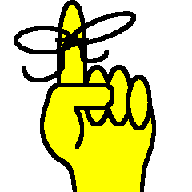
\includegraphics[width=0.7cm]{figures/reminder.pdf}}}}

% Define command to insert gesture image
\newcommand{\gesture}[1]{\marginlabel{{\it#1{\phantom{aa}}}\parbox{1.1cm}{\hspace{-3mm}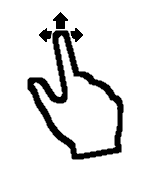
\includegraphics[width=0.8cm]{figures/gesture.pdf}}}}
%
% Define command to insert warning image
\newcommand{\warning}[0]{\marginlabel{\parbox{1.3cm}{
\includegraphics[width=0.9cm]{figures/warning.pdf}}}}
%
% Define command to insert Achtung image
\newcommand{\achtung}[0]{\marginlabel{\parbox{1.3cm}{
\includegraphics[width=2.5em]{figures/warning.pdf}}}}
%
% Define command to insert a flash image
\newcommand{\blitz}[0]{\marginlabel{\parbox{1.3cm}{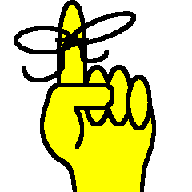
\includegraphics[height=2.0em]{figures/reminder.pdf}}}}
%
% Define command to insert a stop
\newcommand{\halt}[0]{\marginlabel{\parbox{1.3cm}{
\includegraphics[height=2.0em]{figures/warning.pdf}}}}
%
% Define command to reference a configuration item
\newcommand{\config}[1]{\marginlabel{\ref{conf:#1}\parbox{1.3cm}{
\includegraphics[width=0.8cm]{figures/config.pdf}}}}
%
% Potentially overdue ``InfoBox'' style macro but sometimes used... so ..let it be alive ..
\newcommand{\InfoBox}[0]{{InfoBox}}
%
% Define command to put a menu label on the margin
\newcommand{\menulabel}[1]{\marginpar{\parbox{5.0cm}{\raggedright #1}}}
%
% Define command to draw a sketch on the margin
\newcommand{\sketch}[1]{\marginpar{\parbox{4.750cm}{\includegraphics[angle=0,width=0.9\linewidth,keepaspectratio='true']{#1}}}}
%
% Define command to draw a small sketch on the margin
\newcommand{\smallsketch}[1]{\marginpar{\includegraphics[angle=0,keepaspectratio='true']{#1}}}
%
% Enumerated todo's for the todonotes package
\newcounter{todocounter}
\newcommand{\todonum}[2][]{\stepcounter{todocounter}\todo[#1]{\thetodocounter: #2}}
%
% dies nette Makro bringt mir die aktuelle Version der bearbeiteten XCSoar-Verrion aufs Papier 
\newcommand{\version}{\begingroup\catcode`\_=\active\input{VERSION.txt}\endgroup}
%
%Anführungszeichen per Tastatur einfach so eingeben -> "
\shorthandoff{"}%

\def\maketitle{%
  \null
  \thispagestyle{empty}%
  \begin{maxipage}
    \begin{center}
    
\includegraphics[angle=0,width=\textwidth,keepaspectratio='true']{xcsoar-title.png}
    \end{center}
    \begin{center}
      \normalfont\huge\textsf{Glide~Computer and Navigation~System}\par
    \end{center}
    \vskip 1cm
    \begin{center}
      \normalfont\huge\textsf{\@title}\par
    \end{center}
    \vskip 1cm
  \end{maxipage}

  \vfill

  \begin{flushright}
    \large \strut {
      \sf
      \begin{tabular}{r}
      Manual version 1.6 \\
      \today \\
      For XCSoar version 6.0 \\
      \xcsoarwebsite \\
      \end{tabular} 
    } 
    \par
  \end{flushright}
  \par
  \vfil
  \vfil
  \null
  \cleardoublepage
}

\usepackage{makeidx}\makeindex

\begin{document}

%%%%%%%%%%%%%%%%%%%%%%
% Front page
\maketitle

 
%%%%%%%%%%%%%%%%%%%%%%
% Table of contents
\begingroup
\setlength{\cftsecnumwidth}{3em}
\tableofcontents
\endgroup


%%%%%%%%%%%%%%%%%%%%%%
\chapter*{Preface}

\section*{Cuidado e Precauções}

\warning É DE RESPONSABILIDADE DO USUÁRIO QUE FAÇA A
UTILI\-ZAÇÃO DESTE SOFTWARE COM PRUDÊNCIA. ESTE
SOFTWARE TEM O OBJETIVO DE SER UTILIZADO SOMENTE
COMO AUXÍLIO À NAVEGAÇÃO E NÃO DEVE SER UTILIZADO
PARA NENHUM PROPÓSITO QUE NECESSITE MEDIÇÕES
PRECISAS DE DIREÇÃO, DISTÂNCIA, LOCALIZAÇÃO OU
TOPOGRAFIA. ESTE SOFTWARE NÃO DEVE SER UTILIZADO
COMO AUXÍLIO PARA DETERMINAR A PROXIMIDADE COM O
SOLO PARA NAVE\-GAÇÃO AÉREA. ESTE SOFTWARE NÃO DEVE
SER UTILIZADO COMO UM SISTEMA ANTI-COLISÃO AÉREA.



%%%%%%%%%%%%%%%%%%%%%%
\section*{Notas Legais}

\subsection*{Acordo de licença de Software}

Este software é lançado de acordo com a GNU - General Public License
Versão~2. Veja Anexo~\ref{cha:gnu-general-public} para o texto completo do acordo e notas de
garantia.

\subsection*{Responsabilidade Limitada}

Em nenhuma circunstância o XCSoar, ou seus responsáveis, acionistas,
diretores, empregados, afiliados, contratados, subsidiários ou
organizações proprietárias, serão imputados por qualquer incidente,
danos punitivos ou qualquer outro dano relativo ao uso deste produto.

\subsection*{Reivindicações}
Este produto e todos os arquivos que o acompanham, dados e materiais,
são distribuídos “no estado” em que se encontram, sem qualquer
garantia alguma, exceto o que está impresso ou escrito. Este produto
deve ser utilizado sob risco total do usuário. Todavia, foi tomado os
devidos cuidados durante seu desenvolvimento para eliminar defeitos
para ser um produto sem falhas. Nenhuma reivindicação pode ser legal
a respeito da confiabilidade ou aptidão do produto por nenhum
propósito particular. Os projetistas do XCSoar e seus contribuidores não
devem ser responsabilizados por erros internos ou danos, perda de dados
ou injúria pessoal com a conexão com o dispositivo, desempenho ou uso
deste material.


%%%%%%%%%%%%%%%%%%%%%%
\chapter{Einführung}\label{cha:introduction}\index{Einführung@\hypertarget{Einführung}{Einführung}}
Dies ist das \textsf{XCSoar} - Handbuch, geschrieben für \textsf{XCSoar} - Anwender. 

 

\textsf{XCSoar} ist ein Segelflugrechner-Programm, welches ursprünglich einmal für den Segelflugrechner \al der Firma Triadis geschrieben wurde.  
Anschließend waren die vor ca. 10 Jahren aufgekommenen PocketPC das Ziel, in der Zwischenzeit läuft \textsf{XCSoar} jedoch auf fast allen Plattformen und ist derzeit auf Android mit der derzeit 
sehr performanten Hardware zum Laufen gebracht worden. 

Diese Hardware eignet sich ideal, da die allermeisten der Geräte zwischenzeitlich über GPS- und Lagesensoren und einen 
meist recht fixen Prozessor mit entsprechend RAM verfügen, von denen die PDA damals nur zu träumen wagten - und dennoch 
läuft das Program auch dort hervorragend. 


Es wird hier vorausgesetzt, daß der Leser über Grundbegriffe des Fliegens insbesondere des Überlandfluges 
und über die MC-Theorie verfügt, denn ein Lehrbuch für das Fliegen an sich ist das hier nicht.


Es werden regelmäßig Updates herausgebracht, dem Benutzer ist empfohlen, hin und wieder auf der offiziellen Homepage nach zuschauen. 

Man sollte sich die ''release notes'', also die Veröffentlichungen zu den jeweiligen Versionen ansehen, um  auf evtl.\ Änderungen innerhalb des Programmes gefasst zu sein. 
Die komplette Dokumentation ist erhältlich auf  
\begin{center}
\xcsoarwebsite{}
\end{center}
Da \textsf{XCSoar} ein internationales, offenes Projekt ist (an dem jeder mitmachen kann), sind sogut wie alle Vorgänge und Hinweise auf der Homepage auf Englisch. 
Es ist jedoch inzwischen auch ein deutsches Forum gegründet worden, auf dem man sich Informationen holen kann und mit anderen Anwendern über das ein oder anderen auch über Hardware diskutieren kann.
\begin{center}
\url{http://forum.xcsoar.org/viewforum.php?f=14}
\end{center}
oder aber unten auf $<$deutsch$>$ klicken

\section{Einteilung diese Handbuches}
Das Handbuch ist geschrieben, um den Piloten die bestmögliche Unterstützung bzw.\ Einleitung in das Programm zu geben. 
Wir haben uns bemüht, dies vor allem aus Pilotensicht darzustellen (und hoffen, daß das gelungen ist) 

Dies Kapitel beschäftigt sich vor allem mit dem Herunterladen und Installieren des Programmes. 
In Kapitel~\ref{cha:interface} wird auf das Bedienungskonzept eingegangen und soll einen Überblick über das Aussehen des Programmes geben.

Das Kapitel~\ref{cha:navigation} beschreibt die Kartendarstellung ''Moving Map'' im einzelnen  und zeigt, wie das Programm allgemein 
zur groben Unterstützung der benutzt werden kann. Kapitel~\ref{cha:tasks} zeigt auf, wie Überlandflüge geplant, eingegeben, geflogen und gespeichert werden, und bietet eine Übersicht
der Werkzeuge zur Analyse des aktuellen Fluges, um dem Piloten zu helfen,  seine Performance zu steigern.
Im Kapitel~\ref{cha:glide} geht es weiter ins Detail des Segelflugrechners. 
Es ist wichtig, sich mit diesen Details vertraut zu machen, da hier bestimmte Routinen des Programmes erläutert werden.
Externe Sensoren angeschlossener Geräte, Wetter und Atmosphäre werden in Kapitel\ref{cha:atmosph} behandelt, um zu zeigen, wie das Programm 
sich Konvektionsvorhersage, Wind und Thermik in eine \textsf{XCSoar}-interne Wettervorhersage und Flugplanung einbinden läßt.  
Im Kapitel~\ref{cha:airspace} wird beschrieben, wie \textsf{XCSoar} mit Lufträumen umgeht, davor warnt und diese darstellt. 
Weiterhin werden Kollisionswarnungen, welche durch das \fl-System ermittelt werden können behandelt.
Unter dem Abschnitt~\ref{cha:avionics-airframe} wird aufgezeigt, wie sich \textsf{XCSoar} mit diversen anderen Geräten und Systemen 
verbinden läßt z.B.\ auch der Steuerung über externe Schalter wie z.B.\ Wölbklappenschaltern. 

Der Rest des Handbuches beschäftigt sich hauptsächlich mit Referenzmaterial:

Kap.~\ref{cha:infobox} beschreibt die Funktion und den Inhalt der vorhandenen Infoboxen, die auf dem Bildschirm von \textsf{XCSoar} ausgewählt und angezeigt werden können.
Die Konfiguration des Programmes wird in Kap.~\ref{cha:configuration} ausführlich beschrieben. 
Die Formate der einzelnen Files und Daten, welche von \textsf{XCSoar} benutzt, im- und exportiert werden und wo diese zu finden sind, 
wird in Kap.~\ref{cha:data-files} aufgeführt. 

Zum Schluß soll eine kurzer Überblick über die Historie und den Entwicklungsgang von \textsf{XCSoar} zeigen, wie das Programm zu dem wurde, was 
es derzeit ist\dots Bei Interesse: Kap.~\ref{cha:history-development}.

\section{Notes}


\subsection*{Terminologie}
Im Handbuch werden einige Abkürzungen benutzt, welche evtl.\ --aber hoffentlich nicht--  erklärungsbedürftig sind.

So  steht z.B.\  PDA oder ''Organizer'' für eine Reihe von Geräten, welche es mittlerweile schon kaum noch 
gibt, da die Android-Geräte den Markt unglaublich schnell überschwemmen\dots  
{\small Lediglich eine Clique von Segelfliegern deckt sich mit den alten Ipaq ein, da diese für derzeit 15-25Euro in der Bucht 
zu ersteigern und absolut geeignet sind, um mit \textsf{XCSoar} zu funktionieren}

PDA steht für ''Portable Digital Assistant'' (mobiler digitaler Assistent auf rau-Deutsch). 
Ein PNA ist ein ''personal navigation assistant'' also ein ''privater Navigations Assistent ein NAVI!!

Naja\dots Auch die ''organizer'' gehören dazu - also ''Aufräumer'' oder ''Organisierer'' 
 
Egal, und wie auch immer, innerhalb diese Handbuches sollen diese Bezeichnungen lediglich dafür stehen, 
auf welchen Plattformen und Betriebssystemen \textsf{XCSoar} läuft und eine Gruppe von Anzeigeinstrumenten bezeichnen. 

\textsf{XCSoar} gibt es auch für den Triadis \al - Segelflugrechner. 
Für diesen Rechner wurde \textsf{XCSoar} ursprünglich einmal programmiert. Alles, was in diesem Dokument beschrieben wird, wird also auch 
mit dem \al funktionieren (die andere Bedienweise ausgenommen, da der \al kein Touchscreen ist - ebenso wie PC.)

\subsection*{Bildschirmphotos (Screenshots)}

Im Handbuch werden einige Screenshots dargestellt, um die Bedienung/Funktionalität eindrucksvoller und einfacher darstellen zu können.
Natürlich werden sich diese Screenshots von Gerät zu Gerät unterscheiden, wir gehen aber davon aus, daß es nicht sooo 
schwierig sein wird, eine quer-Darstellung  von der Hochkant-Darstellung zu unterscheiden und hoffen, daß im Zweifelsfalle der geschriebene
Text zur Klärung  beitragen wird. 

Es wird daher mitunter Verwirrung geben, da viele der hier aufgenommenen Bilder in der Hochkant-Ansicht aufgenommen wurden 
--wir können nicht für jedes einzelne Gerät entsprechende Screenshots aufnehmen, das würde dies Handbuch auf 400 Seiten aufblähen! 

Wie gesagt, wir versuchen, diese Photos up2date zu halten, es kann aber auch sein, daß mal ein altes bilde auftaucht.

Im Zweifel gilt der geschriebene Text!!!

\section{Plattformen}
\begin{description}
\item[Windows PC]
\textsf{XCSoar} läuft problemlos auf Windows.

Wenn ein GPS angeschlossen und für die Ausgabe der GPS-Daten konfiguriert wurde, kann vollkommen problemlos mit \textsf{XCSoar} gearbeitet 
werden.  (z.B.\ unterwegs auf einem Notebook o.ä.)

Der Simulator läuft ebenfalls vollkommen problemlos, falls keine GPS-Quelle angeschlossen ist!

Jeder, der mit Windows arbeitet und Segelflieger ist (und \textsf{XCSoar} benutzt oder es beabsichtigt), sollte unbedingt die 
PC-Version installieren und am Simulator trainieren!!! 
\item[Windows Mobile PDA/PNA]
PDA und PNA mit Windows mit Microsoft Pocket PC 2003 bis hinzu Windows Mobile 6 laufen mit \textsf{XCSoar} - der Autor hat einen Ipaq3850 seit Jahren 
auch auf Wettbewerben im Einsatz. Es geht!!

Windows Mobile 7 ist nicht unterstützt, da Microsoft entschieden hat, keine Unterstützung für Entwickler dieses 
Betriebssystemes zu geben.
\item[Unix/Linux PC]
\textsf{XCSoar} kann problemlos am WINE-Emulator laufen, es läuft aber auch (seit V6.0x) nativ für die Debian/UBUNTU) Versionen.
\item[Android Devices] \textsf{XCSoar} läuft auf Android 1.6 oder neuer 
\item[\al] Der \al ist ein Segelflugrechner welcher fabrikmäßig mit \textsf{XCSoar} als Software ausgestattet ist. 
Die \al-PRO-Version enthält ein integriertes GPS.
\end{description}


\section{Technische Unterstützung / Support}

\subsection*{Troubleshooting}
Ein kleines Team von freiwilligen, nicht bezahlten Leuten entwickelt und programmiert \textsf{XCSoar}. 

Obwohl wir gerne helfen, können wir nicht jede Frage beantworten, welche sich z.B. mit einem 
Hardware Fehler ''Mein  Galaxy SII bootet nicht mehr'' beschäftigt. Wir denken, das ist unmittelbar einleuchtend.

Es gilt, Software von Hardware zu trennen. 

Wenn Du Fragen zu \textsf{XCSoar} hast, sende eine --konkrete-- mail an: 

\begin{quote}
\url{xcsoar-user@lists.sourceforge.net}
\end{quote}
oder stelle deine Frage auf dem User Forum:
\begin{quote}
\url{http://forum.xcsoar.org/}
\end{quote}

Alle häufig auftretenden Fragen werden gesammelt und zur Website weitergeleitet, wo sie behandelt werden.
Du kannst an die die mailing list schreiben, um aktiv informiert zu werden, sowie Neuigkeiten stattfinden: 

Mehr dazu auf der \textsf{XCSoar}-Homepage. 
\begin{quote}
\xcsoarwebsite{}
\end{quote}

Das beim Start von \textsf{XCSoar} erzeugte log-file \verb|xcsoar.log| ist hilfreich für die Analyse von Fehlern und kann  
mit einem kleinen Bericht zu den Entwicklern gesendet werden, um Fehlern auf die Spur zu kommen 
und \textsf{XCSoar} permanent zu verbessern. 

\subsection*{Updates}
Du solltest periodisch nachschauen, ob Neuerungen/neue Versionen  bzgl.\ \textsf{XCSoar} auf der HP zu finden sind. 
Die Installation ist immer die gleiche; alle vom Bediener erstellten Files wie Konfiguratiobnsfiles 
bleiben beim Update bestehen und können später wieder benutzt werden. Die Updates auf der Android Plattform können -- je nach Einstellungen auf Deiner Hardware  (automatische updates erlaubt\dots)-- vollkommen automatisch erfolgen! 

Nach wichtigen Files wie Karten, Lufträumen und Wegpunkten zu schauen ist wohl selbstverständlich!


Wie jede komplexe Software kann auch \textsf{XCSoar} Fehler enthalten und ist \textsf{XCSoar} darauf angewiesen, daß diese dem Entwicklerteam zur  Kontrolle/Korrektur zugehen. Keine Rückmeldung--keine Verbesserung!

Hierzu gibt es extra ein Bug-tracking-System, also ein Fehler-Verfolgungssystem, in dem Ihr explizit Fehler melden könnt.

Bitte seht vorher nach, ob nicht ein solcher Fehler bereits gemeldet wurde. 
Doubletten machen unglaublich viel Arbeit und behindern den zügigen Fortgang der Entwicklung --logischerweise.  


Hierzu siehe:  
\begin{quote}
\url{https://github.com/XCSoar/xcsoar/issues/}
\end{quote}
oder einfach eine mail an 
\begin{quote}
\url{xcsoar-devel@lists.sourceforge.net}
\end{quote} 

\subsection*{\textsf{XCSoar} auf dem PC benutzen}
Die PC-Version sollte benutzt werden, um es den meisten (Windows)-Usern es zu erlauben, sich mit \textsf{XCSoar} ein 
bißchen auseinanderzusetzen. 

Da die Konfiguration exakt gleich ist, wie auf den mobilen Geräten, sollte es anschließend keine Schwierigkeit geben,
auch mit dem Handy oder PDA mit \textsf{XCSoar} 'abzuheben''.


Die PC-Version kann ebenfalls an externe GPS-Quellen angeschlossen werden und zu einem 
vollwertigen Navigationssystem ''verwandelt'' werden. 


\begin{itemize}
\item Schließe z.B.\ ein \fl an den PC an und benutze diesen als Bodenstation für \fl-Verkehr
\item Schließe den PC an ein intelligentes Variometer an und teste die die Konfiguration damit  (z.B. Vega)
\end{itemize}

\subsection*{\textsf{XCSoar} zusammen mit einem Flugsimulator benutzen und erlernen}
Es ist eine wirklich außerordentlich gute Idee und bringt echt was, \textsf{XCSoar} zusammen mit einem Flugsimulator zu benutzen, bzw.\ zu erlernen.
Dazu muß der Simulator/der PC die Daten mittels des Standard-NMEA-Protokolles ausgeben können, sodaß  \textsf{XCSoar} diese über den seriellen Port auslesen und interpretieren kann.
{\sc Condor} und {\sc X-Plane} bieten derzeit solche Möglichkeiten.  

Der große Nutzen des Trainings am Boden ist der, daß Du in der Luft die Griffe, Interpretationen der Anzeige und Möglichkeiten, 
die Dir \textsf{XCSoar} bietet ''im Schlafe'' beherrscht. Fliegst Du Wettbewerb, so ist das zumindest im Einsitzer absolut unumgänglich.
Auch ein LX8000 ist nicht innerhalb einer halben Stunde (auch nicht innerhalb einer ganzen) zu beherrschen -- und ich weiß wovon ich spreche\dots


\section{\textsf{XCSoar} sicher und verantwortungsbewußt benutzen}
Die Anwendung eines interaktiven Systemes wie  \textsf{XCSoar}, welches sogar Luftverkehrserkennung bietet, läßt den Benutzer dazu neigen, die Luftraumbeobachtung evtl.\ zu vernächlässigen. 
Es ist nicht unsere Intention, Piloten von der Beobachtung des Luftraumes um sie herum abzulenken,  sondern Ihnen  ein Hilfsmittel an die Hand zu geben,
mit dem u.a.\ die Navigation  und die Berechnung  des Endanfluges vereinfacht wird.

Die Philosophie, die hinter der Entwicklung dieser Software steht, ist die, die Ablenkung des Piloten von der Beobachtung wirklich wichtiger Dinge
wie z.B.\ (und vor allem) des in unmittelbarer Nähe befindlichen Luftraumes so gering wie möglich zu halten.

Hierzu ist vor allem Wert darauf gelegt worden, die Bedienereingaben auf ein Minimum --und wenn, dann so einfach und 
schnell wie möglich-- zu beschränken. 
 
Piloten, die  \textsf{XCSoar} benutzen, sollten sich der Verantwortung durch die evtl.\ Ablenkung durch ein solches Programm/System stets bewußt sein!

Es sollte selbstverständlich sein, folgende Dinge zu beachten:
\begin{itemize}
\item Werdet vertraut mit \textsf{XCSoar}, z.B.\ und insbesondere durch die Bedienung des Programmes z.B.\ mit Hilfe des Simulators
\item Benutze und ''fummele'' an Deinem Gerät erst dann herum, wenn Du {\sl sicher bist, daß der Luftraum {\bf frei} ist}!! 
Mache keine Kurven oder Turns, während Du mit der Bedienung der Software beschäftigt bist!An \textsf{XCSoar} herumspielen kannst Du am Boden. 
Du solltest mit der Bedienung wirklich fit sein, gerade auch im Wettbewerb, oder als ''Beginner''.
\item Konfiguriere Dein System so (es ist möglich und Du kannst es\dots), daß Du die interaktiven Eingaben auf ein Minimum beschränkst und 
jederzeit im Griff hast. (Es werden von \textsf{XCSoar} viele automatische Funktionen angeboten - nutze diese oder --falls nicht vorhanden-- 
frage z.B. das Entwicklerteam,  solche Funktionen zu entwickeln/ implementieren).   
\end{itemize}


%%%%%%%%%%%%%%%%%%%%%%
\chapter{Installation}\label{cha:installation}

Um {\textsf  XCSoar} zum Laufen zu bringen benötigst Du folgendes:


\begin{itemize}
\item ein Gerät, auf dem {\textsf  XCSoar} läuft.
\item {\textsf  XCSoar} an sich
\item einen GPS Empfänger
\item ein Wegpunkt-File
\item ein Luftraum-File
\item ein Karten-File (Kartendatenbank bzw. Gelände)
\end{itemize}

\section{Kompatibilität}

\subsection*{Geräte auf denen  {\textsf  XCSoar} läuft}

{\textsf  XCSoar} läuft derzeit auf folgenden Plattformen:

\begin{itemize}
\item Handys und Tablets mit Android 1.6 oder neuer\\
  Beispiel: Dell Streak, Samsung Galaxy S II, HTC Desire HD, Samsung Tablet 10.1N
  Motorola Xoom
\item PDAs mit Pocket PC 2000, 2002, 2003 \\
  Beispiel: Asus A600, Compaq iPaq 3800, 38xx, iPaq 3900, 39xx
\item PDAs mit Windows Mobile \\
  Beispiel: iPaq hx4700, Dell Axim x51v
\item PNAs mit  Windows CE 3.0 oder neuer \\
  Beispiel: HP314, Mio400
\item Triadis Altair
\item LX MiniMap
\item Windows 2000 oder neuer
\item Linux
\item Mac OS X
\end{itemize}

\subsection*{GPS, Logger, Varios}

{\textsf  XCSoar}  ist kompatibel zu allen Geräten, welche GPS-Daten im NMEA-Format ausgeben.

Die meisten modernen Android Geräte haben einen eingebauten GPS-Empfänger, der diese Daten zur Verwendung 
ausgibt. Mitunter jedoch ist es ratsam, diese Daten aus einem anderen Gerät zu verwenden, wenn man z..B.\ Luftverkehrsdaten aus einem 
\fl benutzen und anzeigen möchte oder aber noch weitere Features -wie nachfolgend aufgelistet- nutzen möchte:



\begin{itemize}
\item Geschwindigkeitssensor (TAS) erlaubt schnelle und eine exakte Ermittlung des Winds ohne Kurbeln zu müssen
\item ein extern angeschlossenes Vario wird die Zentrierhilfe unterstützen und erheblich beschleunigen
\item Aufgaben können deklariert und ausgetauscht werden (laden und speichern z.B. in IGC Logger ),   Flüge können ausgelesen werden 
\item manche Varios erlauben eine Synchronisation z.B.\ des MC-Wertes und anderen Werte mit {\textsf  XCSoar} 
\end{itemize}

\subsection*{Unterstützte externe Geräte und deren Funktionen}\label{sec:supported-varios}

\newcommand{\y}[0]{{ $\surd$ }}
%{0.8\textwidth}
\noindent\makebox[\textwidth]{%
\begin{tabular}{l|ccc|cc|cc|c}
       \multicolumn{1}{r}{\bf Unterstütze:} & \multicolumn{3}{c|}{\bf -Funktionen} & \multicolumn{5}{c}{\bf -Daten} \\
NMEA Gerät & 
  \begin{sideways} Deklaration\end{sideways} & 
  \begin{sideways} Fernbedienung\end{sideways} & 
  \begin{sideways} Download\end{sideways} &
  \begin{sideways} TAS \end{sideways} & 
  \begin{sideways} Vario\end{sideways} & 
  \begin{sideways} Baro. Höhe\end{sideways} & 
  \begin{sideways} Wind\end{sideways} &
  \begin{sideways} G-Sensor\end{sideways} \\
\hline

%                    _Decl_Remo_Down_Airs_Vari_Baro_Wind_Gsen_
Borgelt B50          &    & \y &    & \y & \y & \y &    &    \\
CAI 302              & \y & \y & \y & \y & \y & \y & \y & \y \\
CAI GPS Nav          &    &    &    &    &    &    &    &    \\
Condor               &    &    &    & \y & \y & \y & \y &    \\
\hline
Digifly Leonardo     &    &    &    & \y & \y & \y & \y &    \\
EW Logger            & \y &    &    &    &    & \y &    &    \\
EW microRecorder     & \y &    &    &    &    & \y &    &    \\
FLARM                & \y &   & \y  &    &    & \y &    &    \\
\hline
%                    _Decl_Remo_Down_Airs_Vari_Baro_Wind_Gsen_
Flymaster F1         &    &    &    &    & \y & \y &    &    \\
Flytec 5030          &    &    &    & \y & \y &    &    &    \\
GTAltimeter          &    &    &    &    &(\y)& \y &    &    \\
ILEC SN10            &    &    &    &    & \y & \y & \y &    \\
\hline
IMI ERIXX            & \y &    & \y &    &    &    &    &    \\
LX20, Colibri        & \y &    & \y &    &    & \y &    &    \\
LX Vario \footnotemark
                     & \y & \y &    & \y & \y & \y & \y & \y \\

LXNAV Nano           & \y &    &    &    &    &    &    &    \\
\hline
%                    _Decl_Remo_Down_Airs_Vari_Baro_Wind_Gsen_
LXNAV V7             &    & \y &    & \y & \y &    &    &    \\
PosiGraph            & \y &    &    &    &    & \y &    &    \\
Triadis Altair (pro) & \y &    &    &    &    & \y &    &    \\
Triadis Vega         &    & \y &    & \y & \y & \y &    & \y \\
\hline
Volkslogger          & \y &    &    &    &    & \y &    &    \\
Westerboer VW1150    &    & \y &    & \y & \y & \y &    &    \\
Westerboer VW921, 922
                     &    & \y &    & \y & \y & \y &    &    \\
Zander / SDI         &    & \y &    & \y & \y & \y & \y &    \\
\end{tabular}}
\footnotetext{LX Navigation biete mehrere ''intelligente'' Varios an, wie z.B.\ 
  LX1600, LX5000, LX7000. All diese bieten den gleichen NMEA-Ausgang
  Die angebotenen Funktionen in Verbindung mit {\textsf  XCSoar} hängen jedoch zum Großteil auch von der 
Firmware des benutzten  Gerätes ab.}



Während die meisten CE-basierten Geräte über eine serielle Schnittstelle verfügen, 
ist diese Art der Schnittstelle bei den meisten, modernen Android-Geräten nicht mehr vorhanden. 
Diese können entweder Bluetooth oder aber das Android IOIO-Board verwenden. 


Um Bluetooth zu benutzen, verbinde das Gerät mit einem Bluetooth $\leftrightarrow$ Seriell-Adapter, wie z.B.\ 
 dem K6-Bt oder dem Glidertools VFBT-1.


\section{Software Installation der Software}\index{Installation}

Die Software ist auf der {\textsf  XCSoar}-Homepage frei herunterzuladen. 
In diesem Kapitel wird behandelt, {\sl wie} die Software heruntergeladen und installiert wird.

\subsection*{Betriebssystem Android}\index{Installation!unter Android}

Suche nach {\textsf  XCSoar} in Googles Android-Marktplatz (PlayGround), oder installiere das \verb|apk|-
File manuell.  Kopiere diese Datei auf eine SD-Karte in das Verzeichnis \verb|XCSoarData|.

\subsection*{Auf einem PDA (Windows Mobile, PocketPC)}\index{Installation!unter Pocket PC, Windows Mobile}

Wähle eines dieser Files:

\begin{description}
\item[\texttt{PPC2000}] Pocket PC 2000/2002, Windows CE 3.0
\item[\texttt{PPC2003}] Pocket PC 2003, Windows CE 4.0
\item[\texttt{WM5}] Windows Mobile 5 oder neuer
\item[\texttt{WM5X}]Windows Mobile 5 oder neuer mit XScale CPU oder besser(z.B. hx4700)
\end{description}

\sketch{figures/XCS_Today.png}
Lade das File \verb|XCSoar.exe| herunter und kopiere es auf eine SD Karte.  
Starte das File z.B.\ über den Explorer. 

Ein andere Methode ist, {\textsf  XCSoar} auf PDA über das CAB-File zu installieren.  Lade dies File herunter auf Deine SD-Karte, 
anschließend  doppelklicke darauf und {\textsf  XCSoar} wird auf Deinem PDA installiert werden. 

Nach der Installation werden das {\textsf  XCSoar}-Symbol sowie die beiden Schriftzüge ''FLY'' und ''SIM'' aufgelistet
dem ''Heute''-Schirm sichtbar sein. (s.\ Bild) 


\subsection*{Auf einem PNA (Windows CE)}\index{Installation!unter Windows CE}

Lade das File \verb|XCSoar.exe| (Ziel wie oben ''WM5'') auf eine SD Karte herunter. 
Führe es z.B.\ mit dem Explorer aus.

\subsection*{Auf einem Windows PC}\index{Installation!unter Windows}
  
Lade das entsprechende File \verb|XCSoar.exe| (Ziel ''PC'') auf Deinen Rechner (Platte) herunter und führe es aus.


\subsection*{Unter Unix/Linux}\index{Installation!unter Linux}

Das herunterzuladende File ist \verb|xcsoar_XXX.deb|, wobei \verb|XXX| die Version und Plattform darstellt.  
z.B.\ \verb|xcsoar_6.0.4_i386.deb|. Dies ist ein Debian Paket und für 32bit Betriebssysteme mit Intel-Prozessoren gedacht.
Es kann installiert werden mit:
\begin{center}
\verb|sudo dpkg -i xcsoar_XXX.deb|.
\end{center}
Um zu sehen, wo die ausführbaren Dateien und die anderen Dateien installiert wurden, führe \verb|dpkg-query -L xcsoar| 
aus. 

Alle weiteren Dateien (Karten, Lufträume etc.\ müssen in \verb|~/.xcsoar/XCSoarData/| kopiert werden.
Wenn das Verzeichnis \verb|~/.xcsoar| nicht existiert, wird es beim ersten Aufruf von {\textsf  XCSoar} angelegt.


\section{Daten Files}\label{InstallationDatenfiles}\index{Installation!Datenfiles}

Um alle Funktionen von {\textsf  XCSoar} nutzen zu können, werden weitere Daten und Files benötigt.
Hierzu zählen Lufträume, Geländedaten, Topologiedaten eine Polare, Wegpunkte und so weiter. 


Die Nutzung dieser Daten und Files wird in Kap.~\ref{cha:data-files} ausführlich beschrieben. 

Alle Files sollten unbedingt in das Verzeichnis \texttt{XCSoarData} kopiert bzw. \ gespeichert werden. 
Dies Verzeichnis muß  in einem bekannten Verzeichnis befindlich sein, damit {\textsf  XCSoar} bekannt ist, wo es nach entsprechenden 
Daten-File suchen muß: 

 
\begin{description}
\item[Windows PC]
\texttt{XCSoarData} befindet sich im Persönlichen Verzeichnis (''\texttt{Eigene Dateien}'')
\item[Windows Mobile PDA/PNA]
- Wenn ein Verzeichnis \texttt{XCSoarData} im gleichen Verzeichnis wie {\textsf  XCSoar} existiert, dann wird dies benutzt.  


- \texttt{XCSoarData} befindet sich auf der SD-Karte.  Wenn keine SD-Karte vorhanden ist, dann schaut {\textsf  XCSoar} in \texttt{Eigene Dateien} nach diesen Files

\item[Unix/Linux]
Das Verzeichnis heißt \verb|.xcsoar| und befindet sich im \verb|home| - Verzeichnis des Users. 
\item[Android Geräte]
\texttt{XCSoarData} befindet sich auf der SD-Karte.
\item[Altair]
Wenn {\textsf  XCSoar} sich auf einem USB-gerät (Stick) befindet, dann wir dies benutzt, andernfalls wird der interne Speicher benutzt. 
\end{description}


{\textsf  XCSoar} wird während der Laufzeit einige zusätzliche Files, wie z.B.\ eine Datei mit sämtlichen Konfigurationsdetails erzeugen.
Diese werden ebenfalls im \texttt{XCSoarData} Verzeichnis (Windows PC und Windows Mobile Geräte), oder aber im \texttt{.xcsoar} 
Verzeichnis(Unix/LinuxPC) abgelegt. 

Beim ersten Start wird {\textsf  XCSoar}  folgende Files erzeugen und anlegen: 
\texttt{Default.tsk} (Standard Aufgabe),  \texttt{xcsoar-registry.prf} (Konfigurationseinstellungen), \texttt{xcsoar-startup.log} 
(Ein Log-Schrieb des Startprozesses von {\textsf  XCSoar}\dots), 



Weiterhin werden drei Verzeichnisse angelegt: \texttt{cache}, \texttt{config} und \texttt{logs}.  

Während des Laufes von {\textsf  XCSoar} können (und werden) weitere Files angelegt wie z.B.\  Aufgaben-Files (\texttt{*.tsk}) 
und Flugaufzeichnungen (evtl.\ (\texttt{*.igc})


\section{Betrieb von {\textsf  XCSoar}}
%\subsection*{Fly and simulator modes}

{\textsf  XCSoar} wird kann in zwei Modi ausgeführt werden:
\begin{description}
\item[FLY] Dies ist der ''echte'' Flugmodus. Alle Ein - und Ausgänge betr.\ Signalaustausch sind aktiv
\item[SIM] Dies ist der Simulator-Modus. Keine Kommunikation mit externen Geräten per serieller Schnittstelle möglich. 
\end{description}

\subsection*{\al - Version}
Wenn der \al angeschaltet wird, fährt {\textsf  XCSoar} automatisch hoch (es ist quasi das das ''Betriebssystem'' des \al) 
Der PWR/ESC Knopf hat mehrer Funktionen:
\begin{description}
\item[Anschalten]  Drücken und halten für mehr als eine Sekunde: Die LED beginnt zu leuchten und {\textsf  XCSoar} wird starten, nachdem der \al gebootet hat.
\item[Ausschalten]  Drücken und Halten für mehr als drei Sekunden: Schaltet den Altair und somit {\textsf  XCSoar} aus.
\item[Escape] Kurzes Drücken des Knopfes wirkt wie die ESC-Taste eines PC: Wird benutzt als Abbruch-Funktion oder aber zum 
              Ausschalten von von Dialogen benutzt.
\end{description}

\achtung Die \al-Version von {\textsf  XCSoar} hat keine Simulator-Funktion

\subsection*{{\textsf  XCSoar}-PC Version}
Ein Doppelklick im entsprechenden Verzeichnis {\textsf  XCSoar} öffnet das Programm. 
{\textsf  XCSoar} kann auch mit Kommandozeilenoptionen oder über ein Batch-File mit Parametern geöffnet werden, 
die hier angegeben werden: 

\begin{description}
\item[-portrait] Anzeige ist 480 Pixels breit, 640 Pixels hoch
\item[-square] Die Anzeige ist 480 Pixel breit, 480 Pixel hoch
\item[-landscape] die Anzeige ist 640 Pixel breit, 480 Pixel hoch. Dies ist die Standardeinstellung.
Wenn Du nichts anderes angibst, wird diese Einstellung auf dem PC automatisch gewählt.
\item[-small] Dies stellt den Bildschirm in halber Größe dar. sinnvoll z.B.\ wenn {\textsf  XCSoar} in Verbindung mit dem Segelflugsimulator 
{\sc Condor} für das Trainig (oder gegen Langeweile) im Winter gestartet wird.
\end{description}

Um die Bildschirmdarstellung zu ändern ist es sinnvoll, sich in Windows eine Verknüpfung herzustellen. 
In den ''Eigenschaften'' sollte dann unter ''Ziel'' der Programm zusammen mit den Kommandozeilenparametern 
angegeben werden. (z.B.\ \texttt{xcsoar.exe -landscape}


\subsection*{{\textsf  XCSoar} Unix/Linux PC-Version}
Starte \verb|xcsoar| von der Kommandozeile oder aber erzeuge einen Link auf dem Desktop. 

Der Ort, an dem sich die ausführbare Datei befindet,  kann mit \verb|which xcsoar| herausgefunden werden.
Nicht alle Optionen wie bei der PC- Version sind hierbei nun möglich.
 
\subsection*{Nachladen von Daten-Files}
Das erste Mal, wenn {\textsf  XCSoar} gestartet wird, werden {\sl noch nicht} automatisch die Files nachgeladen, welche im 
angegebenen \verb|XCSoarData| abgespeichert wurden. Die kann erst geschehen, wenn {\textsf  XCSoar} das Konfigurationsfeile erstellt hat - also nach dem ersten Start.


Um {\textsf  XCSoar} kenntlich zu machen, wo sich die entsprechenden Files befinden, mache einen kurzen Doppelklick irgendwo auf die nackte Bildschirmfläche 
\sketch{figures/config-basic.png} nach dem Start irgendwo in der nähe des stilistisch abgebildeten Segelflugzeuges in der Mitte, klicke zweimal auf die Schaltfläche ''Konfig'' 
und wähle dann 
\begin{center}
\bmenut{Konfig.}{1/3}~\blink~\bmenut{Konfig.}{2/3}~\blink~\bmenut{System}{Einstellung} 
\end{center}
\achtung {\sl Im folgenden werden die Anzahl der Klicks auf die Menüs wie oben beschrieben nur noch mit {\bf einem} Kästchen dargestellt, d.h.\bmenut{Konfig.}{3/3} steht dann für {\bf 3-maliges Klicken} auf den Konfig.-Knopf
und damit für die dritte Seite des Konfigurations-Menüs}

Auf dieser allerersten Konfigurationseite kannst Du nun unter dem Punkt ''Standortdatei''  die Kartendatenbank, ein Luftraum- sowie ein Wegpunkt-File angeben.
Damit ist {\textsf  XCSoar} bis auf weitere sofort einsetzbar.
viele (wirklich viele\dots) andere Details können anschließend unter \bmenut{System}{Einstellung} an Deine Vorlieben und Bedürfnisse angepaßt werden. 
Die Konfiguration  ist aujsführlich beschrieben in Kap.\ref{cha:configuration} und unbedingt lesenswert. 

Nachdem diese Files hier einmal eingestellt wurden, werde sie bei jedem Start (es sei denn, Änderungen und/oder Neuinstallationen werden vorganommen)
automatisch wieder geladen.

\subsection*{Start-Up und Benutzer Profile}\index{Benutzerprofile}
Beim Start von {\textsf  XCSoar} wird automatisch nach einem Benutzerprofil gesucht. Wenn mehrere vorhanden sind, wird in einem Fenster ganz unten am rande nachgefragt, welcghes file benutzt werden soll.
Aus diesem Grunde macht (wirklich) es Sinn, den einzelnen Benutzerprofilen eindringliche, wiedererkennbare Namen zu geben, 
um diese schnell und eindeutig unterscheiden zu können. 

Wenn kein Profil explizit ausgewählt und geladen wird, wird automatisch das Profile des letzten Startes benutzt. 

Profile können sehr sinnvoll sein z.B. für  

\begin{itemize}
\item verschiedene Piloten
\item eines für Wettbewerbe, eines für Lustflug
\item Fliegen an unterschiedlichen Plätzen (zu Hause, Fliegerlager, Namibia\dots )
\end{itemize}


\subsection*{Simulator Modus (SIM)}
Der Simulatormodus ist entwickelt worden, um mit {\textsf  XCSoar} firm zu werden und bereits vor dem ersten Einsatz im Flugzeug 
Erfahrung mit der Bedienung sammeln zu können. Das unterscheidet {\textsf  XCSoar} von manch anderem fest eingebautem, erheblich teurerem 
 Gerät. 

Im Simulatormodus wird das auf dem Schirm sichtbare Flugzeug ganz einfach gesteuert:
Auf dem TouchScreen (oder mit der Maus), einfach mit dem Finger auf das Segelflugzeugsymbol tippen und in die Richtung 
streifen, wo es hingehen soll. Je länger man zieht/streift, desto schneller wird sich das Flugzeug bewegen. 

In der PC-Version und bei Geräten mit mehreren Knöpfen kann die Geschwidingkeit, Höhe und Richtung mit bestimmten Tasten geändert werdden: 

\achtung {\sl Diese Art der Bedienung ist naturgemäß nicht für TouchScreen-Geräte verfügbar!}


Die Höhe des Flugzeuges kann geändert werden mit einem Druck auf die GPS-Höhe in der \infobox{H GPS}-InfoBox, hier Hoch- und Runter-Tasten benutzen. 

Die Geschwindigkeit des Flugzeuges kann angepasst werden über die Übergrundgeschwindigkeit in der \infobox{V Gnd}-Infobox), hier die Hoch- oder Runter-Taste drücken (oder gedrückt lassen)

Der Kurs des Flugzeuges kann über Kurs-\infobox{Track}-InfoBox, angepasst werden, Hoch- oder Runter -Taste drücken oder halten. 

Wenn entweder\index{Simulator!Steuerung} \infobox{H GPS} oder\infobox{V ü Gnd}) ausgewählt ist, 
kann die Richtung des Flugzeuges auch über die Links- und Rechts-Tasten gesteuert werden.

Alle andere Funktionen, Knöpfe(Buttons) und Menüs arbeiten genau gleich wie im ''FLY'' Modus. 


\subsection*{Start Seite - Ladevorgang}\index{Geduld}
Während des Ladevorganges zeigt {\textsf  XCSoar} einen Ladebalken am unteren Rande des Fensters, 
welche die aktuell geladenen Files und Optionen darstellt. Kann als ''Ladevorgangsbalken'' angesehen werden;  auf PDA $>$ 10Jahre mit dataillierter Kartendatenbank mitunter 
relativ langsam (Geduld-bis zu 90sec können vergehen!!), auf aktuellen Geräten (PC, Android) vergehen meist keine 2 Sekunden (nur beim ersten mal..) 

Diese Seite zeigt auch die Version der Software.

\subsection*{Schließen des Programmes}
Bei PDA und PC-Version, kann {\textsf  XCSoar} vom Menü aus beendet werden. Hierzu Doppelklick auf die Kartenfläche und anschließend 
\begin{quote}
\bmenu{Beenden}
\end{quote}

Beim PC kann auch das ''normale'' Windows-Kreuz genutzt werden.
Der \al wird heruntergefahren und damit {\textsf  XCSoar} geschlossen durch Drücken auf den PWR-Knopf für mehr als zwei Sekunden.




%%%%%%%%%%%%%%%%%%%%%%
\chapter{Interface do Usuário}\label{cha:interface}
\begin{figure}[h]
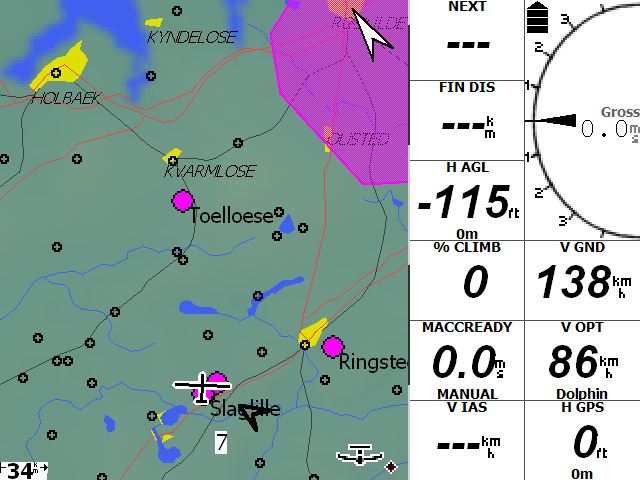
\includegraphics[angle=0,width=\linewidth,keepaspectratio='true']{figures/plain.png}
\caption{Layout mais comum da tela do XCSoar}
\end{figure}

Este capítulo descreve de um modo geral, os conceitos fundamentais da interface do usuário usados pelos XCSoar.  A tela principal mostra a maioria das informações necessárias para o vôo normal.   Geralmente a tela principal é composta de um mapa móvel e infoboxes.  Por várias razões – não é o escopo da introdução – você tem a oportunidade de utilizar várias telas principais, chamadas de páginas de telas.

As páginas de telas são facilmente acessadas por um gesto de deslizamento horizontal, como se tivesse virando páginas de um livro ou por um apertar de botão, dependendo do hardware que estiver usando.  Com a página de telas você estará apto a compor várias telas principais para tirar vantagem da sua utilização em diversas situações de vôo.  Simplificando, você poderá usar a informação apropriada em diferentes casos, podem ser acessadas muito facilmente e rapidamente.

Sempre que alguma situação que pode tirar a atenção do piloto, é mostrada uma informação na tela principal.  Isto acontece especialmente quando há a necessidade de reação do piloto, como uma possível colisão ou quando o piloto irá entrar em uma área de espaço aéreo restrito.

Evidentemente, os botões de menu e menu de telas também são sobrepostos à tela principal.  Como resultado, os elementos apresentados sobrepostos formam uma pilha de exibição com a tela principal representando a base.  As descrições mais detalhadas serão apresentadas nos capítulos seguintes. 


\section{Elementos exibidos}
\subsection*{Tela principal e página de telas}
Cada página de tela do conjunto de páginas do XCSoar é composta de várias partes:

\begin{description}
\item[Área principal] a grande parte da tela é normalmente dedicada à movimentação do mapa do GPS.  Vários símbolos relativos à informação de vôo são sobrepostas ao mapa.  Os ícones e textos devem aparecer ao longo da borda inferior da tela para indicar o estado dos dispositivos conectados, modos de vôo, etc.  De acordo com a evolução do desenvolvimento do XCSoar, há um aumento do número de itens que podem ser escolhidos para serem mostrados na área principal, como medidores FLARM, Radar, Assistente de Termal e Horizonte (como na versão 6.7.2, Dez. 2013).

\item[InfoBoxes] Uma grade de dados é mostrada na parte superior e inferior da tela (formato de retrato da tela), ou do lado direito da tela (formato de paisagem da tela).  São chamados de dados de infoboxes do GPS e outros dispositivos de entrada, bem como podem ter cálculos efetuados pelo XCSoar. Além disso, as Infoboxes podem mostrar também medidores e alguns gráficos.
\end{description}

\subsection*{Sobreposições}
\begin{description}
\item[Instrumentos]  os instrumentos mostram as medições dos sensores.  Todos os instrumentos são opcionais e alguns só poderão mostrar seus dados quando conectados aos dispositivos externos.  A sobreposição do instrumento na tela principal é permanentemente mostrada ou é somente mostrada em algumas condições críticas.  Ex. o assistente de termal é mostrado somente quando o XCSoar entra em modo de giro.  O radar FLARM é mostrado toda vez que há a possibilidade de colisão.  Os instrumentos permanentemente mostrados são a barra de planeio final, bem como a barra de variômetro, entre outros.

\item[Rótulos de Botões e Menus] Os botões do dispositivo que está rodando o XCSoar podem ser usados para navegar em pequenos menus na tela e são normalmente sobrepostos aos menus e podem ser selecionados apertando o botão deste item.  Se o dispositivo possui tela de toque, o item de menu pode ser selecionado clicando sobre o mesmo.  Estes botões são desenhados com texto preto em fundo cinza. 

\item[Mensagem de condição (estado)]o texto é mostrado sobre a tela em uma caixa de mensagens.  Este texto é utilizado para mostrar informações detalhados ao piloto quando alguns eventos ocorrem.

\item[Janela de diálogo] uma grande janela de diálogo, normalmente contendo gráficos e botões são usadas para mostrar dados detalhados ao piloto, relativos aos detalhes de waypoints, estatísticas e análises, etc.

\item[Menu principal] O menu principal é acessado clicando duas vezes na área do mapa ou infoboxes, bem como também por gesto.  Se o menu de botões não for pressionado após algum tempo, desaparecerá da tela para não obstruir a área do mapa. 
\end{description}

\subsection*{Mostrador de vário clássico}
Como dito acima, os mostradores podem ser mostrados de formas diferentes, em infoboxes, sobrepostos ou mesmo na área principal.  O mostrador do variômetro tradicional é diferente.  O mostrador em estilo agulha é mostrado permanentemente, escolhendo o layout da infobox que inclui o variômetro do lado direito das outras infoboxes.

\section{Interação}
Existem várias maneiras de interagir com o XCSoar:
\begin{itemize}
\item Tocando certos elementos no mapa
\item Tocando nas infoboxes e nos botões dos menus da tela.
\item 'Gesticulando', como por exemplo, desenhando um traço da esquerda para a direita na tela (veja seção  \ref{sec:gestures} abaixo).
\item ‘Arrastando’ a tela (tocando a tela e movendo antes de soltar).
\item Apertando os botões de função do dispositivo.
\item Apertando as teclas de cursor do dispositivo.
\item Apertando teclas ou chaves em um dispositivo conectado ao XCSoar.
\end{itemize}

Dependendo do dispositivo conectado ao XCSoar, nenhum destes métodos de interação são possíveis e podem haver números diferentes de funções dos botões.

Para a versão do XCSoar para PC, clicar com o mouse sobre um item tem a equivalência de tocá-lo.

Como o Altair não tem uma tela de toque, todas as interações do usuário são feitas através de botões físicos, chaves ou outro dispositivo conectado.  


\section{O menu principal de botões}
O menu de botões é um conjunto de botões mostrado na tela e ativado por toque ou botões físicos (quando houver no dispositivo).  Esta é a forma primária de interagir com o XCSoar.

\subsection*{A interface básica}
O menu é organizado em quatro grupos diferentes de funções, geralmente em forma de hierarquia.  O layout do menu depende da configuração de botões do hardware e plataforma, e podem também serem personalizados pelo usuário.

O XCSoar pode também aceitar entradas de teclados externos, gamepads, joysticks, etc.  Podem ser atribuídas às estas entradas uma grande variedade de funções.
\sketch{figures/buttonmenu.png}
Para o Altair, há quatro menus principais, ativados por um dos botões físicos verticais do lado esquerdo da tela.  Quando um menu é ativado, uma faixa de botões aparece na parte inferior da tela.  Apertando um botão do menu específico da tecla, irá entrar em várias páginas deste item.  Apertando o botão horizontal correspondente irá ativar o item.  Na última página, apertando o botão de menu novamente, irá desativar este menu e a faixa apresentada na tela desaparece.
Para a versão de PC, estes botões de modo são ativados pelas teclas 1, 2, 3 e 4.  As teclas 6, 7, 8, 9 e 0 correspondem à faixa horizontal de botões.

Na versão PDA, os botões de modo são ativados pelas teclas laterais do joystick.

Se o usuário não interagir com o computador por algum tempo, o menu será fechado automaticamente.  Seu tempo para fechamento é configurável.  A tecla “ESC” no PC ou PWR/ESC no Altair também pode ser utilizada para fechar o menu.

O menu de botões aparece acinzentado se a função correspondente não está disponível.  Por exemplo, se a lista de waypoints aparecer cinza, não há waypoints carregados.
Vários rótulos de botões tem o texto dinâmico baseado em seu contexto, de modo a tornar mais claro o que acontecerá se o botão for pressionado.  A convenção é usada para descrever o que acontecerá se o botão for pressionado. Por exemplo, se o botão descrever \bmenug{MC Auto},portanto, apertando o botão irá deixar o “Auto MacCready” e o texto do botão irá indicar \bmenug{MC Manual}. 
Neste menu descrito acima, são utilizados os rótulos genéricos. 

\subsection*{Menu de funções de grupo}
Esta seção descreve o layout padrão do sistema de menus em todas as plataformas.  As funções desempenhadas por cada botão são descritas com mais detalhes nos capítulos seguintes.

Os botões primários são ativados pelos botões na faixa vertical no Altair, do topo para baixo:

\begin{jspecs}
\item[\bmenug{Nav}] Ações para controle de navegação, provas simples de vôos de cross-country.
\item[\bmenug{Mostrar}]Ações para controle da tela.
\item[\bmenug{Config}] Configuração do XCSoar, dispositivos conectados e ajustes de vôo.
\item[\bmenug{Info}] Ativa várias janelas de diálogo de informações.
\end{jspecs}

Na versão para PC, as teclas 1, 2 3 e 4 ativam os menus correspondentes.  A lista de menus seguinte tem somente o lado esquerdo da maioria dos menus de botões e suas respectivas seções.  Siga-os para verificar todos os detalhes de cada um.

\section{Visão geral do Menu}

\subsection*{Menu de navegação}
\noindent\makebox[\textwidth]{%

\begin{tabularx}{1.44\textwidth}{c|ccccc}
\bmenus{Nav 1/2}
 & \bmenus{Prova}
 & \bmenut{Pto. virada}{Anterior}
 & \bmenut{Próx. Pto.}{Virada}
 & \bmenut{Lista}{Waypoint}
 & \bmenus{Alternativos} \\
see
 & \ref{cha:tasks}
 & \ref{sec:advanc-rest-tasks}
 & \ref{sec:advanc-rest-tasks}
 & \ref{sec:waypoint-selector-dialog}
 & \ref{sec:alternates} \\ \\
\bmenus{Nav 2/2}
 & \bmenut{Prova}{Abortar}
 & \bmenut{Marcar}{Ponto}
 & \bmenus{Alvo}
 & {}
 & {} \\
see
 & \ref{sec:taskabort}
 & \ref{sec:markers}
 & \ref{sec:waypointdetails}
\end{tabularx}}

Você não deve iniciar o uso do XCSoar sem antes saber sobre todas as características do “Alternativos”.  Qualquer “Prova” relacionada no menu de navegação é usada para planejar o vôo de cross-country e certamente será o segundo passo.

\subsection*{Menu Mostrar menu}
\noindent\makebox[\textwidth]{%

\begin{tabularx}{1.44\textwidth}{c|ccccc}
\bmenus{Mostrar 1/2}
 & \bmenut{Zoom}{In}
 & \bmenut{Zoom}{Out}
 & \bmenut{Zoom}{Auto}
 & \bmenut{Info}{Planeio/...}
 & \bmenut{Pan}{On} \\
see
 & \ref{sec:zooming}
 & \ref{sec:zooming}
 & \ref{sec:zooming}
 & \ref{sec:screenpages}
 & \ref{sec:panning} \\ \\
\bmenus{Mostrar 2/2}
 & \bmenut{Rótulos}{All/...}
 & \bmenut{Trilha}{Completo/...}
 & \bmenut{Terreno}{Desligado/...}
 & \bmenut{Topo.}{Desligado/...}
 & \bmenut{Espaço Aéreo}{Desligado/...} \\
see
 & \ref{sec:maplabels}
 & \ref{sec:trail}
 & \ref{sec:terrain_topo}
 & \ref{sec:terrain_topo}
 & \ref{sec:terrain_topo}
\end{tabularx}}

A maioria dos menus mostrados estão disponíveis também com gestos ou atalhos do seu dispositivo.  Assim que estiver mais familiarizado om o XCSoar, provavelmente irá utilizar estes menus com mais freqüência. 

\subsection*{Menus de Configuração}
\noindent\makebox[\textwidth]{%

\begin{tabularx}{1.44\textwidth}{c|ccccc}
\bmenus{Config 1/3}
 & \bmenut{MacCready}{$+$}
 & \bmenut{MacCready}{$-$}
 & \bmenut{MacCready}{Auto}
 & \bmenus{Flight}
 & \bmenus{Vento} \\
see
 & \ref{sec:stf}
 & \ref{sec:stf}
 & \ref{sec:auto-maccready}
 & \ref{sec:flight-setup}
 & \ref{sec:wind-setup} \\ \\
\bmenus{Config 2/3} 
 & \bmenus{SISTEMA}
 & \bmenus{Planador}
 & \bmenus{Dispositivos}
 & \bmenut{File}{Manager}
 & \bmenus{Replay} \\
see
 & \ref{cha:configuration}
 & \ref{sec:glidepolar}
 & \ref{conf:comdevices}
 & {}
 & \ref{sec:logger-replay} \\ \\
\bmenus{Config 3/3} 
 & \bmenut{Registrador}{Iniciar}
 & \bmenus{Raw Logger}
 & \bmenus{Espaço Aéreo}
 & {}
 & \bmenus{Vega} \\
see
 & \ref{sec:logger}
 & \ref{sec:raw-logger}
 & \ref{sec:airspace-filter}
 & {}
 & {}
\end{tabularx}}

O menu de configuração é geralmente parte da interação básica com o XCSoar.  Você não espera perder muito tempo em vôo fazendo ajustes na configuração, com exceção de ajustes de vento ou MacCready.  O item “Vega” fornece controle sobre o variômetro inteligente Vega.  Abrirá um sub-menu.


\subsection*{Menus de Informação}
\noindent\makebox[\textwidth]{%

\begin{tabularx}{1.44\textwidth}{c|ccccc}
\bmenus{Info 1/3}
 & \bmenut{FLARM}{Radar}
 & \bmenut{METAR}{TAF}
 & \bmenut{Oque}{aqui?}
 & \bmenut{Check}{list}
 & \bmenus{Análise} \\
see
 & \ref{sec:flarm-traffic}
 & \ref{sec:metar-taf}
 & {}
 & \ref{sec:checklist}
 & \ref{sec:analysis-climb} \\ \\
\bmenus{Info 2/3}
 & \bmenus{Estado}
 & \bmenus{Meteoro}
 & \bmenut{Time}{Código}
 & \bmenut{Traffic}{List}
 & \bmenut{Assistente}{Termal} \\
see
 & \ref{sec:flight-status}
 & \ref{sec:weather-forecast}
 & \ref{sec:team-flying}
 & {}
 & \ref{sec:thermal-assistant} \\ \\
\bmenus{Info 3/3}
 & \bmenus{Credits}
 & \bmenus{Espaços} {Aéreos}
 & \bmenut{Message}{Repeat}
 & {}
 & {} \\
see
 & \ref{sec:credits}
 & 
 & 
 & 
 &
\end{tabularx}}

O Menu de Informações é sempre um bom referencial, quando não é uma boa dica para ajustar o MacCready, é uma ajuda mais elaborada em um escopo maior para decisões táticas sempre que for necessário para seu vôo.


\subsection*{O Sub-menu de Configuração do Variômetro Vega}
\noindent\makebox[\textwidth]{%

\begin{tabularx}{1.44\textwidth}{c|ccccc}
\bmenus{Vega 1}
 & \bmenut{Airframe}{Switches}
 & \bmenut{Setup}{Audio}
 & \bmenut{Manual}{Demo}
 & \bmenut{Setup}{Stall}
 & \bmenus{Accel} \\ \\
\bmenus{Vega 2}
 & \bmenut{ASI}{Zero}
 & \bmenut{Accel}{Zero}
 & \bmenus{Store}
 & \bmenut{Cruise}{Demo}
 & \bmenut{Climb}{Demo}
\end{tabularx}}

As funções deste sub-menu requerem o variômetro inteligente Vega.  O menu pode ser acessado somente se o ‘Veja” for selecionado como dispositivo conectado.

\subsection*{O modo panorâmico do sub-menu do Menu Mostrar}

\noindent\makebox[\textwidth]{%

\begin{tabularx}{1.44\textwidth}{c|ccccc}
\bmenus{Pan}
 & \bmenut{Pan}{Off}
 & \bmenut{Zoom}{in}
 & \bmenut{Zoom}{out}
 & \bmenut{Oque}{aqui?}
 & {} \\
see
 & \ref{sec:panning}
 & {}
 & {}
 & {}
 & {}
\end{tabularx}}

Este sub-menu infelizmente se sobrepõe à tela principal no modo Panorâmico.  Suas funções são evidentes, todavia o menu pode ser reposicionado por tecnologia multi-toque ou botões (como no Altair).  Porém, juntamente com o botão “Pan Off” também há o botão “O que aqui?” que oferece um ótimo acesso à variedade de informações do mapa.

\section{Botões de Menu padrões}

Quando não há menu ativo (chamado de modo padrão), uma linha de botões no Altair desempenha as seguintes funções (da esquerda para a direita):

\begin{center}
\begin{tabular}{c c c c c c}
 PC: & 6 & 7 & 8 & 9 & 0 \\
 Altair: & F5 & F6 & F7 & F8 & F9 \\
& \bmenus{Flight} & \bmenut{Task}{Manager} & {} & \bmenus{Alvo} & \bmenut{Marcar}{Ponto} \\
\end{tabular}	
\end{center}

Teclando ESC no Altair mostra os rótulos para estes botões.
Para outras versões no modo padrão, o cursor faz as seguintes funções:

\begin{jspecs}
\item[Tecla Acima] Zoom +
\item[Tecla Abaixo] Zoom -
\item[Tecla esquerda] Marcar ponto
\item[Tecla direita] alterna entre as infoboxes normais e auxiliares e tela cheia
\item[Enter] Limpa a mensagem de estado ou suprimi o mostrador FLARM se estiver aberto e se nenhuma mensagem de alerta estiver ativa.  
\end{jspecs}

Para a versão Altair em modo padrão, o botão rotativo desempenha as seguintes funções:
\begin{jspecs}
\item[Botão rotativo externo sentido anti-horário] Zoom +
\item[Botão rotativo externo sentido horário] Zoom -
\item[Botão rotativo interno sentido anti-horário] (Sem função atribuída)
\item[Botão rotativo interno sentido horário] (Sem função atribuída)
\item[Aperta botão rotativo] Limpa a mensagem do estado ou alerta de espaço aéreo.
\end{jspecs}

Nos formulários de diálogo, o botão rotativo no Altair desempenha as seguintes funções:
\begin{jspecs}
\item[Botão rotativo externo sentido anti-horário] Cursor para cima
\item[Botão rotativo externo sentido horário] Cursor para baixo
\item[Botão rotativo interno sentido anti-horário] Cursor esquerdo
\item[Aperta botão rotativo] Cursor direito
\item[Aperta botão rotativo] Tecla Enter
\end{jspecs}

Para o Altair, os botões ao longo da borda da tela podem ser usados como formas alternativas de navegação nos diálogos.  A tecla F4 (diretamente acima do botão rotativo) pode ser usada com um ENTER alternativo (ao invés de pressionar o botão rotativo) nos diálogos.  As teclas F6 e F7 (à direita do botão rotativo) podem ser usadas para selecionar a próxima página ou a anterior nos diálogos multi-páginas.

\subsection*{Rótulos dinâmicos de menu}
Certos menus têm rótulos dinâmicos para tornarem mais claro o que ocorre quando um menu for selecionado.  Além disso, itens que não estão disponíveis estão acinzentados para indicar que esta seleção não terá efeito algum.

A convenção usada para rótulos dinâmicos de menus é para rótulos que mostram a ação que será desempenhada quando o item do menu for selecionado.  Por exemplo “Luzes Acessas” irá ligar as luzes e o menu aparecerá “Luzes Apagadas” que só se apagarão se o menu for pressionado.  Esta convenção é usada no também no XCSoar.

Uma seleção de teclas de menus dinâmicos é mostrada abaixo:

\begin{description}
\item[\bmenug{Próx. Pto. Virada}]  
 Se acinzentado, a prova foi limpa ou se o ponto ativo foi finalizado.  Se estiver ativo, é o ponto principal para o final, e estará indicando “Waypoint finish”.
\item[\bmenug{Pto. virada anterior}]  
  Acinzentado se a prova foi limpa, ou se o ponto ativo é o início (start) e não há mais pontos de início.  Se houver múltiplos pontos de início e o pilão é o “start”, então aparecerá descrito “Cycle Start” para permitir a seleção entre os vários pontos de início.  Se o pilão ativo é o primeiro ponto após o início, aparecerá descrito “Waypoint Start”. 
\item[\bmenug{Rótulos Todos}]  
 Desta forma irá mostrar todos os rótulos disponíveis no mapa.  Há mais opções de visualização que mostrarão um pequeno número de rótulos como “Rótulos Prova”, não poluindo demais a tela.
\item[\bmenug{Alvo}]  
  Acinzentado se a prova foi limpa ou a prova abortada.

\end{description}


\section{InfoBoxes e páginas de telas}\label{sec:infoboxandpages}

A informação indicada nos campos da infobox podem ser selecionadas em uma grande variedade de opções (listadas no Capítulo 12).  Estes campos podem também ser utilizados por exemplo, para ajustes de MacCready.

O número específico e layout da grade da infobox depende da orientação da tela e do tamanho da tela do dispositivo.
Para uma tela de 320x240 de um Pocket PC em modo retrato, há quatro Infoboxes acima e quatro abaixo da tela de mapa.

Um layout normal de paisagem tem 9 infoboxes e o mostrador do variômetro do lado direito da tela.  Para telas maiores, podemos ter até 24 infoboxes mostrados simultaneamente.
\sketch{figures/infoboxes.png}

Para se ganhar clareza, quanto menos infoboxes você escolher para serem visualizados, mais fácil será a leitura dos mesmos.  Por outro lado, há muitas e muitas opções de infoboxes que o piloto não rejeitaria.  A quantidade de números possíveis de opções para Infoboxes excede 100 opções.  Por este motivo que o XCSoar oferece duas maneiras de gerenciar ainda mais opções do que o número de infoboxes.

Dependendo do seu estado de vôo, quando estiver girando ou voando reto, você pode deixar o XCSoar alterar o conteúdo de cada infobox.  Como exemplo, você deve mudar a infobox que mostra a média de subida na termal enquanto está girando para uma infobox que lhe informe a velocidade quando estiver voando reto.  Esta mudança é derivada automaticamente entrando em diferentes modos de vôo (seja seção 6.1), executando a mudança para outra janela de infobox.

Mais ainda, você pode usar as páginas de tela para mudar o conteúdo da Infobox manualmente, assumindo diferentes conjuntos na infobox para páginas diferentes (veja a seção seguinte).

Para ter acesso à mudança automática de infobox de acordo com o tipo de vôo, deixe o XCSoar rodar um o conjunto pré-configurado da instalação.  Para ajustar sua própria versão de infoboxes, siga o procedimento:

\begin{description}
\item[Geometria da InfoBox] escolha o layout da infobox.  O layout básico é mantido através de qualquer mudança no vôo, influenciando somente o conteúdo da infobox.
only.\config{interface-appearance}
\item[Escolha Infobox "Auto"] Configure pelo menos uma página de tela com a escolha de Infobox “Auto”.  Como pode ser visto na tela configuração correspondente, há mais páginas de telas pré-definida.  As demais não são necessárias para terem alternância automática. 
\item[Defina os conjuntos de ajustes da Infobox] Agrupe o conteúdo da infobox que deseja que seja mostrada em três páginas de infobox chamada de “Girando”, “Planeio” e “Planeio Final”, respectivamente.
\end{description}
 

 
\subsection*{Página de telas com diferentes conjuntos de infobox}\label{sec:screenpages}

XCSoar permite que o piloto defina os vários conjuntos de infoboxes que forem apropriados para o vôo normal.  Assume girando, voando ou planeio final como normal, o XCSoar pode alterar as infobox correspondentes automaticamente.

Como pode imaginar, há inúmeros casos de conjuntos que podem ser mostrados.  Você pode ter até oito conjuntos de páginas de telas, refletindo a situação atual.  Algumas possibilidades são dadas, só para fazer um breve resumo do uso do conceito da página de telas.

\label{par:use_case}
\begin{description}
\item[Familiarização] se você é um piloto de ponta, você está procurando obter os benefícios dos inúmeros cálculos e provas que o XCSoar pode fornecer.  Para ter estes benefícios relacionado às fases da competição, deve aceitar a idéia de definir dois casos especiais de páginas, para a fase de início, outra para a prova.  Se você procura por um valor específico para ser mostrado, vá ao capítulo  \ref{cha:infobox} "Infobox reference". 
Há grande chance de achar lá.
\item[No chão] Como um gerenciador, você deve usar uma página de tela mostrando o “Radar FLARM” somente.  Pode acontecer na tela do PC rodando o XCSoar conectado a um receptor FLARM.
\end{description}

Qualquer que seja o que gostaria de mostrar, leve em conta o momento de uso e o conceito de página de telas.

\gesturespec{left}
Para ir através de várias páginas de telas, use as teclas esquerda/direita (Altair) ou gestos esquerda/direita (tela de toque) através do botão de menu \bmenug{Mostrar 1/2}, mostrando um rótulo dinâmico, mudando de acordo com o conteúdo da página de tela para mostrar o próximo:
\gesturespec{right}

\bmenut{Mostrar}{1/2}\blink\bmenut{Assistente de}{Térmica}\blink\bmenut{Info}{Planeio}\blink\bmenut{Info Planeio}{Final}\blink\bmenut{Info}{...}


\subsection*{Modificando o conteúdo da InfoBox }

(This section applies only when a touch-screen or mouse is present.)

S(Esta seção somente se aplica se houver tela de toque ou mouse presente).  Alguns valores de infobox podem ser alterados pelo usuário selecionando (ex. longo pressionamento) o dado no infobox na tela de toque ou mouse.  Aparecerá uma caixa de diálogo pequena:

\begin{description}
\item[\bmenuw{Editar}]  
Permite ao piloto ajustar a infobox (ex. aumentar ou diminuir o ajuste de MacCready)

\item[\bmenuw{Config}]
 Permite que se mude o comportamento do ajuste da infobox (ex. alterando de “auto” para “manual” o modo de MacCready); ou alterando a própria infobox teclando “Mudar Infobox” e então escolhendo uma lista de infoboxes disponíveis.

\end{description}

Os exemplos de infoboxes podem ser ajustados incluindo o ajuste de MacCready, velocidade do vento e altitude (QNH).


\subsection*{Modificando o conjunto de Infobox}

(Esta seção só se aplica quando há uma tela de toque ou mouse.)
Um conjunto inteiro de infobox pode ser composto pela configuração do sistema em “Aparência” e “Pages”, também na seção 13.22.  As caixas de diálogo fornecem uma grande variedade de ajustes e configurações para as páginas do XCSoar.


\section{Status messages}

As mensagens de estado aparecem sobre a área do mapa para mostrar um texto num curto período de tempo.  A mensagem desaparece após um período de tempo configurado e tipos diferentes de mensagens tem períodos diferentes.  As mensagens de estado também podem ser configuradas para desaparecerem após confirmação da mensagem.  A confirmação pode ser feita tanto pressionando a tecla ENTER (botão rotativo no Altair), tocando na mensagem de estado (nos dispositivos com tela de toque) ou clicando na tela (com o mouse).

Botões adicionais do usuário podem ser configurados para confirmar a mensagem e repetí-la.
As mensagens mais comuns são

\sketch{figures/status-message.png}

Typical status messages include:
\begin{itemize}
\item Questões de espaço aéreo
\item Alertas de espaço aéreo
\item Eventos de interface do usuário (ex. mudança da tela)
\item Eventos de alteração de cálculos de vôo (ex: decolagem, pilões)
\end{itemize}

Note que as mensagens de estado não aparecerão se houver uma janela de diálogo aberta na tela.  As mensagens são enfileiradas e serão mostradas assim que a janela de diálogo for fechada.  


\section{Janela de diálogo}\label{sec:dialog-windows}

O XCSoar contém várias janelas de diálogos que podem ser ativadas para trazer informações adicionais e também usadas para uma interação mais complexa com o usuário, como editar provas e configurar ajustes.
Alguns diálogos simplesmente mostram informações e não requerem ação do usuário.  Outros diálogos contêm campos de dados que podem ser modificados ou botões que podem ser pressionados.
Um cursor aparecerá sobre o botão ativo ou o campo de dado.  Teclando nas setas acima/abaixo (ou rotacionando o botão giratório do Altair), o cursor irá circular através do item próximo ou prévio.  Para listar os itens e textos, a tecla acima/abaixo move o cursor acima ou abaixo da lista ou texto, e as setas esquerda/direita move o cursor acima ou abaixo de uma página em uma lista longa.
Para PDAs e versões para PC, os itens listados podem ser selecionados tocando o item (ou clicando com o mouse).  Quando um item na lista é selecionado, outro toque (ou clique) é equivalente a pressionar a tecla ENTER.
Teclando as setas direita/esquerda (ou rotacionando o botão rotativo interno no Altair), o valor do campo de dados sob o cursor pode ser modificado.  Teclando ENTER (ou apertando o botão rotatório no Altair), ativa o botão ou faz a seleção da lista.
As janelas de diálogo normalmente se iniciam através do botão Menu.
A maioria das janelas de diálogo têm múltiplas página de informações e são controladas de uma forma consistente.  Tecle \bmenuw{$<$}> ou \bmenuw{$>$} para selecionar a página próximo ou prévia do diálogo e CLOSE para fechar.
A tecla ESC no PC ou PWR/ESC no Altair também podem ser usada para fechar as janelas de diálogo.
O usuário deve fechar as janelas de diálogo para retornar a visualização do mapa.  Quando um diálogo for aberto, o botão principal de menu é desativado até que o diálogo seja fechado.
Em alguns diálogos, os itens que não relevantes ou inválidos (como detalhes AAT quando se voa uma prova não-AAT) não são mostrados.
 Abaixo é apresentado um resumo dos principais diálogos.

\begin{description}
\item[Ajuste de Vôo] usado para modificar a polar da aeronave antes e durante o vôo, bem como ajustar a pressão QNH.
\item[Vento] usado para modificar ou ajustar a velocidade estimada do vento e sua direção. 
\item[Detalhes de Waypoint] Descreve o detalhe do waypoints e tem a função de “Ir Para” e “Inserir na Prova”
\item[Lista de Waypoint] usado para selecionar um waypoint do banco de dados de waypoints
\item[Gerenciador de Prova]Use-o para criar, modificar e visualizar as provas de cross country
\item[Análise] Use-o para criar, modificar e visualizar as provas de cross country
\item[Estado] A janela de estado fornece um resumo da situação da aeronave, sistema, prova, inícios e tempos.
\item[Configuração] Permite a configuração do XCSoar e certos dispositivos conectados.
\item[Filtro de espaço aéreo] Controla a ativação e desativação das notificações e alertas de cada classe de espaço aéreo.
\item[Código de time] Permite transferir as coordenadas entre o time FLARM via código
\item[Dispositivos]  Seleciona os vários dispositivos externos (ex. variômetro, FLARM, etc).
\item[Ajuste Planador]  Fácil reconfiguração dos ajustes da aeronave (ex. polar, ID do competidor, etc.) escolhendo de uma lista de aeronaves previamente criadas
\end{description}

Estes diálogos são descritos em capítulos posteriores, com exceção da checklist, estado e caixas de diálogo com estrada de textos, que são descritas abaixo.


\subsection*{Check-list (exemplo de diálogo}\label{sec:checklist}

A janela de checklist pode ser mostrada em diversas páginas definidas pelo usuário.  Geralmente é usada para checklist e podem ser acessadas através do menu.

\bmenut{Info}{1/3}\blink\bmenut{Check}{List}
\sketch{figures/checklist.png}

Esta checklist pode incluir: inspeções diárias, pré-vôo, pós-pouso, pré-pouso, procedimentos de rádio, ancoragem e desancoragem da aeronave.
Se a check list for longa, as teclas acima/abaixo (ou botão rotativo no Altair) podem ser usados para rolar através do texto.  Clicando em \bmenuw{$<$} e \bmenuw{$>$} seleciona a próxima ou prévia checklist.



\subsection*{Entrada de texto} \label{sec:textentry}

Uma janela de texto é usada para entrada de texto.  Pode ser usada para entrada de código de time, ajustes de nome de arquivos, edição de waypoints, bem como entrar outras opções de configuração, como o nome do piloto para o registrador.

Duas formas de entradas de texto são permitidas.  

Para alterar o tamanho do texto, use os botões 
\sketch{figures/textentry.png}
para ajustar o caractere sobre o cursor. Clicando nos botões the \button{$<$} 
e \button{$>$} move o cursor para esquerda/direita.  

Para entrar um texto com a tela de toque, aperte as letras uma após outra.  Em algumas janelas (ex. edição de waypoints) somente as letras que coincidem com uma entrada no banco de dados será mostrada.  Para apagar a última letra, use\button{$<-$} \sketch{figures/textentry_keyboard.png}. A tecla \button{$CLEAR$} apaga toda a entrada.

Pressione \button{$OK$} para finalizar ou \button{$CANCEL$} para sair. 



\section{Alertas acústicos e retorno de som}

O XCSoar gera sons para eventos diferentes e podem ser configurados para ter sons personalizados para cada evento.  Veja seção 14.13 para detalhes desta personalização.

Quando o XCSoar é conectado ao variômetro inteligente Vega, envia um comando ao sistema de voz do Vega para fornecer alertas sonoros como:

\begin{itemize}
\item Planeio final através do solo
\item Aproximando/passando pelo waypoints de uma prova
\item Alertas de espaços aéreos
\end{itemize}

A interface do usuário do XCSoar também pode conectar um retorno de som ao completar qualquer comando como por exemplo:
\begin{itemize}
\item Ponto marcado.
\end{itemize}


\section{Screen visuals}

Certos aspectos da aparência dos itens na tela podem ser ajustados.  O mais comumente configurado é a visualização das infoboxes e mostradores em branco e preto (chamado de cores inversas), ou preto e branco.
Para os controles da tela do Altair, o brilho pode ser ajustado conforme abaixo:


For Altair the control of the screen hardware 
\sketch{figures/brightness.png}
brightness can be controlled from the brightness dialogue.
\begin{quote}
\bmenug{Mostrar 2}\blink\bmenug{Brilho}
\end{quote}

Consulte {\em Altair Manual do Usuário's Manual} para detalhes da janela de brilho.


\section{Sistema de ajuda}

Um sistema de ajuda fornece um texto descritivo das propriedades para a maioria dos comandos.  Quando há a seleção de uma propriedade, para o Altair, aperte e segure o botão \button{$ENTER$} por 2 segundos e solte. Abrirá uma janela com um texto de ajuda descrevendo a propriedade.  

\section{Interfacing with gestures}\label{sec:gestures}
A partir da versão 6.0, o XCSoar aceita “gestos”

Para usar esta característica, seguro o dedo na tela (ou botão do mouse no PC), desenhe 
uma figura e solte a tela ou o botão do mouse.  Dependendo do que for desenhado, será 
ativada uma função específica. \sketch{figures/gesture1.png}

Um gesto específico é definido pelos movimentos dos dedos ou cursor nas quatro direções 
Cima, Baixo, Esquerda e Direita.  Significa que se você arrastar seu dedo para baixo e 
depois para a direita na tela, \gesture{dr} o gesto “BD” (baixo e direita) é detectado e 
está configurado para mostrar a lista de waypoints
 
O manual indica os gestos disponíveis mostrados aqui no lado esquerdo do corpo de texto.  Ambos os pictogramas do movimento e a mão azul são utilizados para indicar um gesto específico, neste caso movendo para baixo e para direita.  A lista com os movimentos disponíveis é mostrada abaixo. \gesturespec{dr}
\vspace{2em}

\subsection*{Gestos básicos mais comuns:}
\begin{itemize}
\item[\raisebox{-1em}
{
\includegraphics[angle=0,width=0.1\linewidth,keepaspectratio='true']{figures/du.png}}] BC, denotando uma marca de seleção: mostra o Menu principal
\item[\raisebox{-1em}
{
\includegraphics[angle=0,width=0.1\linewidth,keepaspectratio='true']{figures/up.png}}] C: Zoom +
\item[\raisebox{-1em}
{
\includegraphics[angle=0,width=0.1\linewidth,keepaspectratio='true']{figures/down.png}}] B: Zoom -
\item[\raisebox{-1em}
{
\includegraphics[angle=0,width=0.1\linewidth,keepaspectratio='true']{figures/left.png}}] E: Muda a tela para cima (Normal, Aux., tela cheia)
\item[\raisebox{-1em}
{
\includegraphics[angle=0,width=0.1\linewidth,keepaspectratio='true']{figures/right.png}}] D: Muda para a tela anterior (Normal, tela cheia...)
\item[\raisebox{-1em}
{
\includegraphics[angle=0,width=0.1\linewidth,keepaspectratio='true']{figures/urdl.png}}] E, escrevendo “P”: modo Panorâmico.  Também pode ser ativado movendo-se dois dedos na tela.
\end{itemize}
\vspace{2em}

\subsection*{Mais gestos disponíveis:}
\begin{itemize}
\item[\raisebox{-1em}
{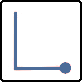
\includegraphics[angle=0,width=0.1\linewidth,keepaspectratio='true']{figures/dr.png}}] BD, escrevendo um “L”: mostra a lista de Waypoints 
item Waypoint \textbf{L}ist
\item[\raisebox{-1em}
{
\includegraphics[angle=0,width=0.1\linewidth,keepaspectratio='true']{figures/rd.png}}] DB, escrevendo um “T”: abre o gerenciador de provas
\item[\raisebox{-1em}
{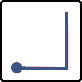
\includegraphics[angle=0,width=0.1\linewidth,keepaspectratio='true']{figures/dl.png}}] BE: mostra a lista alternativa
\item[\raisebox{-1em}
{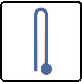
\includegraphics[angle=0,width=0.1\linewidth,keepaspectratio='true']{figures/ud.png}}]CB: ativa o Auto Zoom
\end{itemize}
\vspace{2em}

\subsection*{Gestos sofisticados:}
\begin{itemize}
\item[\raisebox{-1em}
{
\includegraphics[angle=0,width=0.1\linewidth,keepaspectratio='true']{figures/urd.png}}] CDB, escrevendo um “A”: mostra janela de análises
\item[\raisebox{-1em}
{
\includegraphics[angle=0,width=0.1\linewidth,keepaspectratio='true']{figures/ldrdl.png}}]EBDBE, escrevendo um “S”: mostra a janela de Estado. 
\end{itemize}


%%%%%%%%%%%%%%%%%%%%%%
\chapter{Navigation}\label{cha:navigation}
This chapter describes the moving map display as an aid to navigation,
and also describes some of the task and glide related overlays on the
map display.

\section{Map display elements}

\begin{maxipage}
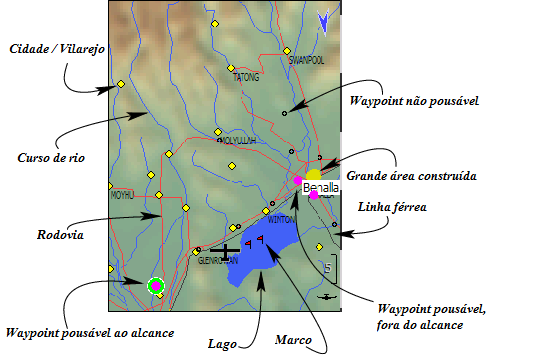
\includegraphics[angle=0,width=0.9\linewidth,keepaspectratio='true']{figures/fig-map.png}
\end{maxipage}

The moving map shows:
\begin{enumerate} 
\item Glider symbol
\item Waypoints
\item The active task
\item The bearing (or route\footnote{The line to the next waypoint may be a {\em route}, as described in Section~\ref{sec:route}.})
  to the next waypoint
\item Special Use Airspace
\item Terrain and topology
\item Markers
\item Trail
\item Glide range\footnote{The glide range is also referred to as the {\em reach}, as described in Section~\ref{sec:reach}.}
\end{enumerate}
The map is drawn in a projected coordinate system (not latitude and
longitude), and the scale can be changed (zooming in and out), as well
as panned.  All navigation functions take the curvature of the Earth
into account.

\section{Glider symbol, map orientation}
The glider symbol shows the position of the glider on the map.  The
orientation of the glider indicates the estimated heading of the
glider.

The map is oriented in one of three ways: North up,
Track up, or Target up.  Configuration settings \config{orientation} can be used
to specify a different map orientation when in circling mode. This is useful to prevent
disorientation when looking at the map while circling.  Target-up when
circling makes it easy to determine which direction to exit the
thermal.

When Track or Target-up is used in circling mode, the glider symbol is
centred on the screen, even if the symbol position is configured differently.
In cruise mode the Track and the Target-up orientation allows the glider
symbol to be positioned (e.g.) 20\% from the bottom of the screen, giving a good view of the
map ahead of the glider.  This position is adjustable in the configuration
\config{gliderposition} settings.

\section{Zoom and map scale}

To change the scale of the map, for PC, PNA, or Pocket PC:
\begin{enumerate}
\item Tap/click on a blank part of the map to highlight the map if it is not
already selected.
Then use mouse wheel, or the Pocket PC up/down key to either zoom
in or out.
\item You can also gesture to change the zoom level. Gesture \gesture{Up/Down}
``Up'' zooms in, ``Down'' zooms out.
\item A PNA with a button wheel let you also change the zoom. 
\item Or select the function from the menus:
\begin{quote}
\bmenu{Display}\blink\bmenu{Zoom In} and \bmenu{Display}\blink\bmenu{Zoom Out}
\end{quote}
\end{enumerate}
On Altair, the rotary knob can be used to zoom in and out.

The map scale is displayed in the lower left corner of the moving map
display. The incicated distance is measured from the left to the right boarder
of the map display.
\marginpar{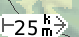
\includegraphics[angle=0,width=0.4\linewidth,keepaspectratio='true']{figures/zoom.png}}

Compaq Aero Users. If you enable the Compaq Aero Game Keys (On the
Q-menu) the centre two front buttons become the up/down keys.

There is a facility to have two zoom settings; one when the glider is
in circling mode, and one in the cruise or final mode.  This is the ``Circling
zoom'' option in the \config{circlingzoom} configuration settings.  
By default, the circling zoom is set to about 2.5 km - 5.0 km, depending on the
display size. When the user zooms in or out, it affects the current
mode's zoom setting only, so when leaving the mode the previous mode's
zoom setting is used.  If ``Circling Zoom'' is not enabled,
there is only a single zoom level.

Auto-zoom automatically zooms in when approaching a waypoint to keep
the waypoint at a reasonable screen distance. When auto-zoom is active,
'AUTO' appears next to the map scale. The user can still zoom
in and out if desired, zoom will be switch to manual control automatically.
\marginpar{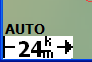
\includegraphics[angle=0,width=0.4\linewidth,keepaspectratio='true']{figures/zoomauto.png}}

To turn auto zoom on or off, select from the menu
\begin{quote}
\bmenu{Display}\blink\bmenu{Display}\blink\bmenu{Zoom Auto} 
\end{quote}

When a waypoint changes (automatically, via the task selector, or by
manually switching waypoints), auto-zoom adjusts the zoom level
automatically so that the next waypoint is visible on the map.


\section{Panning the map}

A pan mode allows the user to explore areas beyond the glider.  This
is particularly useful when task planning.
\begin{enumerate}
\item Enable pan mode by pressing 
\begin{quote}
\bmenu{Display}\blink\bmenu{Pan On}
\end{quote}

\item The map can then be panned by dragging the screen or using the cursor
  keys.  For Altair, panning is performed with the inner/outer rotary knob.
\item When done, pan mode has to be disabled manually, by pressing:
\begin{quote}
\bmenu{Pan Off}
\end{quote}

\end{enumerate} 

When pan is active, the text 'PAN' appears next to the map scale.  While
pannig the location of the focus stays in the middle of the display under the
cross hairs.

A special menu of buttons in pan mode is also displayed when in pan
mode.

\begin{center}
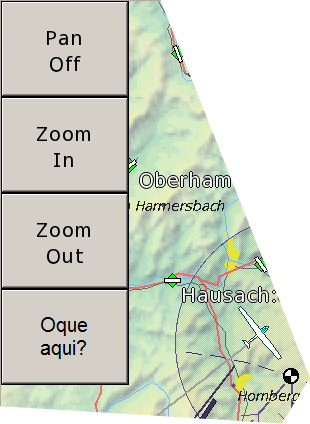
\includegraphics[angle=0,width=0.8\linewidth,keepaspectratio='true']{figures/pan.png}
\end{center}

\section{Waypoints} \label{sec:waypoint-schemes}
Waypoints are displayed with different symbols depending on the
waypoint type; the major distinction being landable and non-landable
waypoints.

The waypoint symbols are drawn as shown below There are three icon sets for
landable waypoints. \config{waypointicons}

\begin{tabular}{c|c|cc|cc|}
Icon set &\begin{sideways}Simple waypoint\end{sideways}
&\begin{sideways}Landable field\end{sideways}
&\begin{sideways}reachable\end{sideways}
&\begin{sideways}Aerfield\end{sideways}
&\begin{sideways}reachable\end{sideways}\\
\hline
Purple Circle &
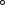
\includegraphics[width=0.5cm]{icons/map_turnpoint.pdf} &

\includegraphics[width=0.8cm]{icons/winpilot_landable.pdf} &

\includegraphics[width=0.8cm]{icons/winpilot_reachable.pdf} &
\colorbox{white}{
\includegraphics[width=0.8cm]{icons/winpilot_landable.pdf}}
& 
\includegraphics[width=0.8cm]{icons/winpilot_reachable.pdf} \\
\hline
B/W Icon & 
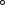
\includegraphics[width=0.5cm]{icons/map_turnpoint.pdf} &

\includegraphics[width=0.9cm]{icons/alt_landable_field.pdf} &

\includegraphics[width=0.9cm]{icons/alt_reachable_field.pdf} &
\colorbox[rgb]{0.94,0.94,0.94}{
\includegraphics[width=0.9cm]{icons/alt_landable_airport.pdf}}
& 
\includegraphics[width=0.9cm]{icons/alt_reachable_airport.pdf} \\
\hline
Orange Icon & 
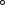
\includegraphics[width=0.5cm]{icons/map_turnpoint.pdf} &

\includegraphics[width=0.9cm]{icons/alt2_landable_field.pdf} &

\includegraphics[width=0.9cm]{icons/alt_reachable_field.pdf} &
\colorbox{white}{
\includegraphics[width=0.9cm]{icons/alt2_landable_airport.pdf}}
& 
\includegraphics[width=0.9cm]{icons/alt_reachable_airport.pdf} \\
\hline
\end{tabular}


Waypoints are optionally labelled according to one of several
abbreviation schemes. \config{labels}

XCSoar continually calculates which landing points are within gliding
range using the current wind estimate.  The estimated arrival altitude
{\em above the arrival safety height} of reachable landable points is
displayed next to the waypoint.  This arrival altitude is calculated
with the glider performance and MacCready setting configurable as
either that of the task\config{reachpolar}, or at a safety MacCready value.

\section{Active task}

The active task course is drawn on the map as a green dashed line.
Assigned area tasks also show the task sectors or areas as a yellow shaded
region.  
Circles are always drawn around start and finish points, lines are
only drawn if the start/finish points are of line type.  Task
observation sectors are drawn as segments.

At all times a thick black line is drawn from the glider to the next
waypoint in the task.  This line may be the direct path to the waypoint,
or may be a {\em route} path clearing terrain and airspace obstacles, described in
further detail in Section~\ref{sec:route}.

\begin{center}

\begin{tabular}{c c c}
{\it Start/finish} & {\it Sector} & {\it Cylinder} \\
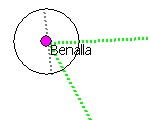
\includegraphics[angle=0,width=0.3\linewidth,keepaspectratio='true']{figures/cut-startfinish.png} &
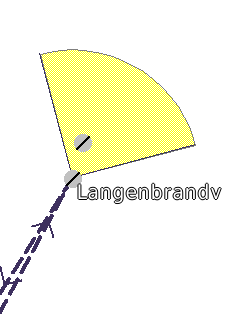
\includegraphics[angle=0,width=0.3\linewidth,keepaspectratio='true']{figures/cut-sector.png} &
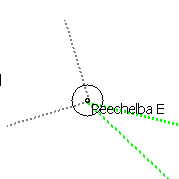
\includegraphics[angle=0,width=0.3\linewidth,keepaspectratio='true']{figures/cut-barrel.png} \\
\end{tabular}
\end{center}

\section{Terrain and Topology}

The following topological features are drawn on the map:
\begin{itemize}
\item Major roads, shown as red lines
\item Rivers, shown as blue lines
\item Large water bodies (lakes), shown as blue areas
\item Large cities, shown as yellow areas
\item Small population areas, shown as yellow diamonds
\end{itemize}
Cities and small population areas are labeled in italics.

Terrain is coloured according to height, and optionally shaded by sun
direction or lift-generating slope.  Invalid terrain, or terrain below
sea level is coloured blue.

Terrain is shaded to improve visibility.  Currently the shading
is set up so that the virtual lighting position is the wind bearing,
thus brighter areas are on the upwind side of hills and dark areas in
the lee of the hill.  The amount of shading and overall terrain
brightness is configurable.  Support for a sun ephemeris is underway.
Terrain shading and brightness can be configured \config{shading}.

Both terrain and topology display can be switched on or off from the
menu:
\begin{quote}
\bmenu{Display}\blink\bmenu{Display}\blink\bmenu{Terrain On} \\
\bmenu{Display}\blink\bmenu{Display}\blink\bmenu{Topology On}
\end{quote}

\begin{center}
\begin{tabular}{c c}
Topology & Terrain \\
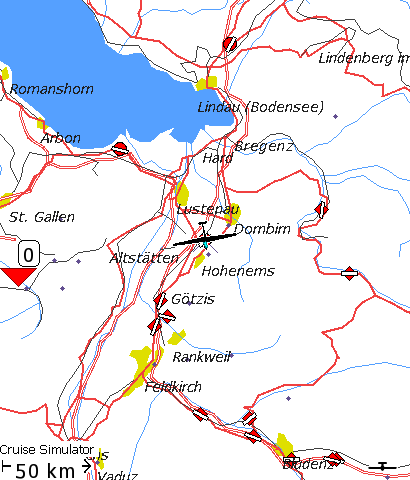
\includegraphics[angle=0,width=0.4\linewidth,keepaspectratio='true']{figures/cut-topo.png} &
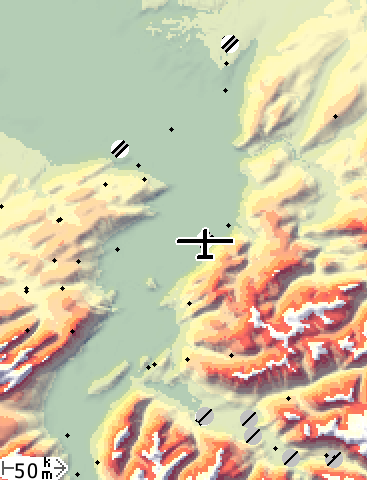
\includegraphics[angle=0,width=0.4\linewidth,keepaspectratio='true']{figures/cut-terrain.png} \\
\end{tabular}

\end{center}

If the terrain data is not available (or terrain display is turned
off), the background colour of the map window is white.  All terrain
below mean sea level is coloured blue.  If you are flying outside the
terrain region, the background colour will be white.

The screen can be de-cluttered, turning off the display of topology
labels and non-task waypoint labels by toggling:
\begin{quote}
\bmenu{Display}\blink\bmenu{Display}\blink\bmenu{Labels Off}
\end{quote}


\section{Trail}\label{sec:trail}

An optional 'snail trail' is drawn on the map showing the glider's
path history.  The colour and thickness of the trail depends on the height or
on the variometer value. \config{snailtype} 

\begin{center}
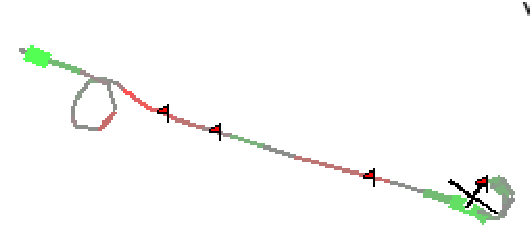
\includegraphics[angle=0,width=0.8\linewidth,keepaspectratio='true']{figures/snail.pdf}
\end{center}

If Vega or an intelligent variometer is connected with Netto output,
the Netto vario value is used; hence the colours and thickness of the
trail indicates the air-mass vertical movement rather than the glider's
vertical movement	.

The snail trail display can be toggled between off, a short trail
(about ten minutes), a long trail (about one hour) or a full trail
which displays the entire flight.  This can be performed permanently
through the configuration \config{snailtrail} settings or temporarily by the
menu:
\begin{quote}
\bmenu{Display}\blink\bmenu{Display}\blink\bmenu{Snail trail}
\end{quote}

Note that for all of these modes, the snail trail is short in
circling mode in order to reduce screen clutter.

In order to assist centering thermals in the presence of wind, the
snail trail can be artificially drifted with the wind as it is
displayed (this is drift compensation).  In this way, the snail trail
is referenced to the prevailing wind rather than referenced to the
ground.  Since thermals drift with the wind also, the drifted trails
give a better indication of where the glider has been relative to the
thermals.

An example of this is illustrated below.  Note that when trail drift
compensation is active (right picture), the glider appears to be
circling in a column rather than an elongated spiral (left picture).

\begin{center}
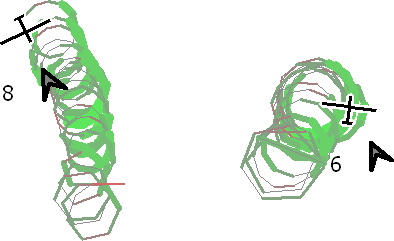
\includegraphics[angle=0,width=0.8\linewidth,keepaspectratio='true']{figures/traildrift.png}
\end{center}

Enabling trail drift compensation is performed through the
configuration settings \config{traildrift}.  The compensation is only performed
whilst in circling mode; the display of the trail in cruise mode is unaffected.
This can also be performed from the wind settings dialog:
\begin{quote}
\bmenu{Config}\blink\bmenu{Setup Wind}
\end{quote}

The trail drift display is useful also to show more clearly when thermals
are cranked due to wind shear.

The trail width can be adjusted in the configuration settings \config{trailwidth}.

\section{Markers}

\begin{tabular}{c}%{c}

\includegraphics[angle=0,width=0.75cm,keepaspectratio='true']{icons/map_flag.pdf}\\
(a)
\end{tabular}


Markers are shown as small flags (a) on the map.  The markers can be dropped
manually, by pressing a button, or automatically.  An example use of
automatic markers is to drop markers when entering circling mode, as a
simple way of showing all thermals encountered.

Markers are not preserved after XCSoar is exited, however the location
of all marks are appended to the file \verb|xcsoar-marks.txt|.

Markers are dropped by the menu, or by gesture \gesture{Left}: 
\begin{quote}
\bmenu{Display}\blink\bmenu{Mark Drop}
\end{quote}

\section{Glide range line}\label{sec:reach}

A reachable glide `footprint' is displayed on the map display as a
black and white dashed line, indicating where the glider would descend
through the terrain clearance height.  The reach shows clearance
tracks extending in all directions, optionally including paths around
terrain obstructions.  This feature is useful in assessing range with
respect to topology when searching low for lift, and when flying in
mountainous areas.

Reach calculations may be configured \config{turningreach} to two levels of detail:
\begin{description}
\item[Straight line] If turning reach is disabled, then the reach shows the
 furthest distance the glider can fly in final glide in all directions without
 turning.  This reach appears as a closed ring around the glider.

\begin{center}
\includegraphics[angle=0,width=1.0\linewidth,keepaspectratio='true']{figures/reach1.png}
%{\it DIAGRAM CUTOUT SHOWING GLIDE RANGE FOOTPRINT.  NO TOPOLOGY,
%FULLSCREEN, NO TASK. TURNING=FALSE}
\end{center}

\item[Turning] If turning reach is enabled, then the reach shows the
  greatest area the glider can reach in all directions, even allowing
  turns around obstructions.\footnote{The maximum number of turns is
    set to three, and no turns may be greater than 90 degrees.}  The
  reach area appears as a closed ring around the glider but may also
  include holes indicating mountain peaks that the glider cannot reach
  without further climb.

\begin{center}
\includegraphics[angle=0,width=1.0\linewidth,keepaspectratio='true']{figures/reach2.png}
%{\it DIAGRAM CUTOUT SHOWING GLIDE RANGE FOOTPRINT.  NO TOPOLOGY,
%FULLSCREEN, NO TASK. TURNING=TRUE}
\end{center}

\end{description}

The display can be configured to additionally blur the unreachable area
outside the glide range. \config{gliderange}
The final glide path is checked for whether the glider clears terrain along
the path by the terrain clearance height.  If clearance is not attained, a red
cross appears on the map at the point where the violation occurs. If a target is
defined the calculation is done along the path to the target. 

If reach is enabled, then the reachability of landable waypoints is used
by the abort task mode, alternate landable option lists and display of
landable waypoints on the map.

Note that task calculations are otherwise unaffected by reach
calculations --- for example, heights required as shown in the final
glide bar or task data as displayed in infoboxes do not take reach into account.

Furthermore, the reach calculations are used for footprint, landable
waypoint arrival heights, abort mode and the alternates dialog.  The glider
performance and MacCready setting used in these calculations are configurable\config{reachpolar}:
\begin{description}
\item[Task] The MC value is that used in the task.
\item[Safety MC] A configurable, typically low MC value is set by the user to set
 performance near, but slightly degraded to, best glide performance.

\end{description}

\section{Status dialog}\label{sec:aircr-stat-dial}

The nearest landmark function, typically available via the button
menu, brings up a status message describing the name, distance and
bearing to the nearest landmark.  The nearest landmark is also
reported on the status dialog.

You may find this function useful when you need to report your
location to others.

Currently the landmarks scanned are the list of waypoints.  In the
future, XCSoar may also search for nearby towns and cities in the
topology database.

The aircraft status dialog (see Section~\ref{sec:dialog-windows})
shows the status of the aircraft's locality, and can be useful when
giving position reports.

This is accessed via the menu under: 
\begin{quote}
\bmenu{Info}\blink\bmenu{Info}\blink\bmenu{Status}.
\end{quote}
and then selecting the page `Aircraft'.

\section{Route}\label{sec:route}

XCSoar can plan paths around terrain and airspace obstacles in three
dimensions from the aircraft to the destination.  Such a path is known
as a route.  The height of the destination is the arrival height for
final waypoints, or may be higher for intermediate waypoints, as
dictated by the task system as required to complete the task.  Route
planning functions in normal ordered task mode, abort mode and goto
mode.

\begin{center}
\includegraphics[angle=0,width=1.0\linewidth,keepaspectratio='true']{figures/route3.png}
\end{center}

Routes take into account the glider polar performance and are
calculated to be optimal in the sense of minimum time.  By default,
route calculation is disabled, and can be enabled for terrain only or
terrain and airspace avoidance \config{routemode}.

Terrain is avoided vertically by the terrain safety height
\config{safetyterrain}, with no additional lateral clearance imposed.
Valid routes may result in the aircraft arriving at the destination
higher than the minimum height --- such as can occur when the
destination is just beyond a steep mountain.

Airspace is avoided horizontally by a buffer of approximately 250 m,
with no additional vertical clearance imposed.  Valid routes may fly
below or above airspace.

If MacCready is positive, then climbs are optionally allowed
\config{routeceiling} in the computed routes.  The top of the climb
may be limited to 500 m above the heigher of the start and destination
ceiling, or increased to the ceiling defined by the thermal ceiling
\config{routeceiling}.  Climbs above the higher of the start and
destination altitude are penalised by a slower climb rate than the
actual MacCready value.

Some approximations and limitations of the route planning system are as follows:
\begin{itemize}
\item Where climbs are necessary (and permitted) to reach the destination,
the climbs are assumed to occur at the start of the route.
\item Climb-cruise segments are assumed to occur at constant altitude,
equivalent to many small climbs distributed along the path.
\item Individual turns between path segments greater than 90 degrees
  are not permitted.
\item Failures of the solver result in the route reverting to direct flight
from the aircraft location to the destination.
\end{itemize}



%%%%%%%%%%%%%%%%%%%%%%
\chapter{Cross Country Tasks}\label{cha:tasks}

XCSoar provides a full task management system, in which tasks can be
edited prior to flight and, when undertaking casual cross-country
flying, modified during flight.  Waypoints are advanced automatically
or may be cycled through manually.  This chapter also describes the
use of IGC loggers with XCSoar.

There are three task modes available:
\begin{description}
\item[Ordered task] This is the natural cross-country task type,
in which the task consists of a start point, zero or more waypoints,
and a finish point.  The task points are to be flown in order.
\item[Goto task] Flight to a single destination.
\item[Abort task] Provides options to fly to the nearest landing points.
\end{description}

Note that in goto and abort modes, the ordered task is retained and may be resumed
later, preserving any statistics about achievement in the task.

\section{Goto tasks}

Goto tasks may be established by selecting a waypoint from the map,
the waypoint list, or any other mechanism e.g. the alternates dialog,
\gesture{Down - Left} and select ``Goto''.  In goto task mode, selecting
\bmenu{Nav}\blink\bmenu{Task resume} resumes the ordered task (if
any).

\subsection*{Automatic goto}

If no ordered task is defined, then on takeoff, a goto task is automatically
established with the takeoff point as the destination, or the nearest airfield
if it was close to the takeoff point.

Whether or not a task is defined, the takeoff point is always
generated and appears in the waypoint list for later reference or use.

\section{Editing tasks}

You can edit tasks in several ways.  Some methods are more useful for
editing prior to flight, and others allow tasks to be modified whilst
in flight for casual cross-country touring.  Tasks can be saved to
files and loaded later, and can be transferred between any XCSoar
platform (Pocket PC, Altair, PC).

\tip It is also possible to save a `default' task and have this task loaded
automatically upon start-up of XCSoar.  One application of this is to
set up a default task with one waypoint being the home --- this means
that XCSoar is then programmed for final glide back to home, which is
useful for casual cross-country touring.

The main ways of setting tasks are the following:
\begin{itemize}
\item Using the task editor dialog
\item Selecting waypoints from the map and adding them to the task from the
 waypoint details dialog
\item Loading the task from a file
\end{itemize}

%Selecting the Task menu item will produce the Task dialog box.  The
%list box on the left displays all of the turn points loaded into the
%system. Highlight the desired entries and using the "-$>$" and "$<$-"
%buttons assemble the desired task in the Task list box. As each turn
%point is added to the task a continuous display of the calculated task
%length is shown.  Tasks can be saved for recalling later using the
%"Save" button and recalled using the "Load" button.  Once the desired
%task is complete select "OK".
%
%{\it DIAGRAM SHOWING TASK DIALOG EDITING, WITH LABELED ARROWS POINTING
%TO THE USER INTERFACE ELEMENTS?}

\tip Loading a task from file may be useful in competition or casual
cross-country flying in groups, as one person can distribute the task
file to others, thereby saving the group the job of editing the task
themselves.

%\tip If no task is present at startup, a task is created automatically,
%  containing one waypoint to home.
% There will be a 6.1 feature like this.

XCSoar saves the current task when shutting down and loads it at
startup, thereby allowing the task to be entered early in the day,
then the device running XC Soar can be turned off until flight time.

Task waypoints are preserved even if the waypoint
file is changed.  This means, if you save a task, then change the
waypoint file, then load the task again, new waypoints are generated
for any waypoints that are missing in the new waypoint file.

\section{Waypoint Info dialog}
%Several ways of selecting a waypoint are available:
%\begin{itemize}
%\item Touch its name or the waypoint symbol on the map screen if it is visible.
%\item If the waypoint is in the active task, highlight the waypoint {\InfoBox}, then use the up/down arrow keys to select the desired waypoint, and press the
%enter key.
%\item From the Task dialog, find and highlight the waypoint in
% the waypoint list, then press the 'Details' button.
%\end{itemize}
%The display will now show the waypoint details dialog.

The waypoint info. dialog describes a waypoint in detail and has
navigation functions such as GoTo, Insert or append to the task, and set the waypoint as the new home..

This may be accessed several ways:
\begin{itemize}
\item
From the task editor, menu \bmenu{Nav}\blink\bmenu{Task}\blink\bmenu{Turn Points}
and highligh a waypoint, then tap the highlighted waypoint again to display the Task point dialog, then press the \bmenu{Details} \InfoBox.

\item 
From the menu \bmenu{Info}\blink\bmenu{Waypoint details} to show the
details for the active waypoint.

\item
From the menu \bmenu{Info}\blink\bmenu{Nearest waypoint} to show the
details of the waypoint nearest the aircraft, or if in pan mode,
nearest the pan cursor.

\item
From the waypoint selector, menu \bmenu{Nav}\blink\bmenu{Waypoint
List} and select a waypoint to show the details of that waypoint.

\item
If the waypoint is visible on the screen, touch its name or the waypoint symbol


\end{itemize}

The waypoint details dialog contains two major pages (accessed via the
\button{$>$} and \button{$<$} buttons). Depending on the availability of further
details to the waypoint they will by shown on extra pages.

\subsection*{Waypoint details}
This page contains text describing the waypoint's location, radio frequency and runway information (if this information is in the waypoint file) elevation, local sunset, bearing and distance to the waypoint, and the altitude required to reach the waypoint as described below. In addition, there is a button \button{GoTo} to directly initiate
navigating to this waypoint. The button cancels the current task. 
\begin{center}
\includegraphics[angle=0,width=0.8\linewidth,keepaspectratio='true']{figures/dialog-waypointdetails0.png}
\end{center}

As mentioned above, the Waypoint info dialog also shows three forms of altitude difference (additional
altitude required to reach the waypoint at the safety height) for
the corresponding waypoint:
\begin{description}
\item[Alt diff MC 0] Altitude difference at MC setting of 0
\item[Alt diff MC safety] Altitude difference at the abort/safety MacCready setting (see \ref{sec:Safety factors})
\item[Alt diff MC current] Altitude difference at the current MacCready setting
\end{description}

From the main Waypoint Info screen, you can access the second page by using the "$<$-" and "$-$>" buttons in the bottom left corner of the page.
\subsection*{Task menu}  
This page contains a column of buttons allowing various actions to be performed:
\begin{description}
\item[\button{Replace in task}] replaces the active waypoint in the task with the selected waypoint.
\item[\button{Insert in task}] inserts the selected waypoint before the active waypoint in
  the task.
\item[\button{Append to task}] adds the selected waypoint to the end of the task.
\item[\button{Remove from task}] removes the selected waypoint from the task.  Note that this option is only visible if the selected waypoint is included in the active task.
\item[\button{Set as new home}] sets the waypoint as the home airfield.
\item[\button{Set teamcode}] sets the waypoint as reference waypoint for
  team code coordinates.
%I don't see this last box, but I don't have FLARM.  Is this box only visible if you have FLARM, or was it removed?%


\end{description}

It is a good idea to set your home waypoint from the waypoint details
dialog. This causes XCSoar to start up at the home location regardless
of whether a GPS fix is received.  If no home is set, then XCSoar
starts in the center of the terrain map.

\subsection*{Airfield information}
This page may contain relevant text from the enroute supplement about
the airfield, including runways, radio frequencies, traffic patterns,
contacts.
\begin{center}
\includegraphics[angle=0,width=0.8\linewidth,keepaspectratio='true']{figures/dialog-waypointdetails1.png}
\end{center}

\subsection*{Satellite image}
This page shows a satellite image of the
waypoint.

%I don't have a screen for the Satellite image.  Has this feature been removed, or is it because I haven't loaded the satellite images into the waypoint datafile?  Where is this documented?%

\begin{center}
\includegraphics[angle=0,width=0.8\linewidth,keepaspectratio='true']{figures/dialog-waypointdetails2.pdf}
\end{center}


\section{Waypoint selector dialog}\label{sec:waypoint-selector-dialog}
The waypoint selector is a dialog that allows waypoints to be easily selected
from a potentially large database.

This may be accessed several ways:
\begin{itemize}
\item  From the menu \bmenu{Nav}\blink\bmenu{Waypoint List}
\item  From the task editor, menu \bmenu{Nav ..}\blink\bmenu{Task
Edit} and selecting a waypoint and open the details.
\item  Or just by gesture\gesture{Down - Right}.
\end{itemize}

The waypoint selector comprises a set of optional filters on the left
side of the page, and a list of matching waypoints on the right.
There are several filters available, which may be used together,
individually or not at all.
\begin{description}
\item[Name] Filtering based on the matching the first letter in the waypoint name. 
\item[Distance] Filters out waypoints further that a specified distance to the aircraft.
\item[Direction] Filters out waypoints that are not in a specified direction from the aircraft. 
   An additional special direction ``HDG(0°)'' filters waypoints within 30
   degrees to either side of the heading of the glider.  This allows the pilot to point the glider at a group of
  waypoints and quickly find them.
%Filtering by heading doesn't seem to work as described. Need more explanation here.%
\item[Type] Filters out waypoints that are not of the specified type
(Landable point, Airport or Turnpoint) or that appear in the specified File~1 or
File~2 (primary or secondary waypoint file respectively).
\end{description}
When filtering by name and type, the list of matching waypoints is
sorted by name. When (in addition) filtering by distance or direction,
 the list of matching waypoints is sorted by distance.

\begin{center}
\includegraphics[angle=0,width=0.8\linewidth,keepaspectratio='true']{figures/dialog-waypointselect.png}
\end{center}

The list can be scrolled if there is more than one screen full of
matching waypoints.  To scroll through the list, simply drag with the finger, or
move to the bottom (or top) of the list with the cursor.   

Selecting an item will result in different behaviour
depending on what function opened the waypoint selector.  In typical
use it brings up the waypoint details dialog for the selected
waypoint.

\section{Task manager}\label{sec:task-manager-dialog}
\begin{it}The task manager has undergone significant redesign compared with earlier versions of XC Soar.\end{it}

The task manager is used to edit, view, load, save to file, and declare cross
country tasks. It is accessed via the menu
\begin{quote}
\bmenu{Nav}\blink\bmenu{Task}
\end{quote} 

The task manager's primary page is an calculator. It shows various calculations related to the active task, as described in detail below.  In addition, there are buttons for \button{Calculator}, \button{Turn Points}, \button{Manage}, and \button{Rules}, as well as a button to \button{Close} the task manager.

\subsection*{Turn Points}
The \button{Turn Points} button displays an ordered list of the points in the current active task.  If there are no waypoints in the active task, there will be only an option to "Add Turnpoint."  By highlighting (tapping) the "Add Turnpoint" function, then tapping in the highlighted region, the waypoint selector is displayed, as described above.  Highlighting a waypoint from the list and then tapping on the highlighted region adds the waypoint to the task.

\subsection*{Manage}
Tapping on the \button{Manage} button displays the task manager's management screen.  There are four options, each of which is accessed by tapping on the relevant button:

\begin{itemize}
\item \button{New Task} Clears the current task and resets the task rules to the default values.
\item \button{Declare}  If an external logger is connected, this will allow uploading the  active task to the logger and declaring it.
\item \button{Browse} Displays a list of all the saved tasks, allowing the pilot to load a previously saved task.  Note that this option will overwrite the current active task.
\item \button{Save}  Saves the current active task.  Upon tapping the \button{Save} button the pilot will be prompted to enter a file name for the task to be saved.
\end{itemize}

\subsection*{Rules}
The values in the \button{Rules} menu depend on the task type selected.  Clicking any existing value will bring up another menu allowing the pilot to select a different value for this rule.  Task types are discussed in more detail below.

Also, tapping on the \button{Rules} button again after it is highlighted allows toggling between a "thumbnail" view of the task map and a larger view of the task.

\subsection*{Task types}
XC Soar currently defines three different task types: Racing, AAT, and FAI badges/records.

A brief description of the task types is included below, but this manual does not intend to rephrase FAI rules or contest task types.  The reader is encouraged to become thoroughly familiar with each task type by referring to contest rules or FAI rules, which are available at \url{http://www.fai.org}. 

\begin{itemize}
    \item Racing (also known as an "assigned task").  The racing task involves flight around each specified turnpoint in the specified order.  Selecting the racing task type allows the pilot to enter the following parameters (note: if the option "FAI start/finish rules" is set to "On" then none of the options are available %Why is this?%:
\begin{itemize}
    \item Start max. speed: This is the maximum speed allowed in the start observation zone.  This should be set to 0 if there is no limit.
		\item Start max. height: This is the maximum height above the start height reference (AGL or MSL) at which a task can be started.  This  should be set to 0 for no limit.
	\item Start height referece: This specifies whether the maximum start height is referenced to ground level of the start point ("AGL") or Mean Sea Level ("MSL")
	\item Finish Minimum Height: This is the minimum height based on the finish reference (AGL or MSL) at which a task can be finished.  This should be set to 0 for no limit.
	\item Finish height referece: This specifies whether the minimum finish height is referenced to ground level of the finish point ("AGL") or Mean Sea Level ("MSL")
	\item FAI start/finish rules: If enabled, this task type has no max start height or max start speed.  Finish height reference is set to AGL and finish height is 1000m below the start height %Is this description correct?%
\end{itemize}
\item AAT (also known as "Turn Area Task,"or TAT).  This is a task through assigned areas (restricted to cylinder or sector observation zones).  A minimum task time applies.  Rules options for this task type include:
\begin{itemize}
    \item AAT minimum time:  This is the required minimum time for the task.  Refer to contest rules or consult an expert for penalties associated with finishing prior to the minimum time.  The time in this option is given in minutes.
	\item Start maximum speed: Same meaning as in the racing task type, above
	\item Start maximum height: Same meaning as in the racing task type, above
	\item Start height reference: Same meaning as in the racing task type, above
	\item Finish minimum height: Same meaning as in the racing task type, above
	\item Finish height reference: Same meaning as in the racing task type, above
	\item FAI start/finish rules: Same meaning as in the racing task type, above
\end{itemize}
\item FAI badges/records.  This task type allows only FAI start, finish, and turn point types.
\end{itemize}

Once the appropriate task type has been selected and start and finish rules have been defined as described above, it is necessary to define the properties of each waypoint in the task.  Waypoints can be start points, turnpoints, or finish points.

This is defined by tapping the \button{Turn Points} button from the Task Manager.  This brings up the list of waypoints in the task (if any).  Highlighting any waypoint on the list and either tapping it again or pressing the \button{Edit Point} button brings up the waypoint definition pressing the \button{Change type} button  will bring up a menu of the various task point types available.  Definitions of each point type are shown below the list.

%Need to add a section describing how to start the task%

\section{Advancing and restarting tasks}\label{sec:advanc-rest-tasks}
At all times one waypoint in the task is designated as the active
waypoint.  The active waypoint is used for calculation and display of
navigation information, that is, the pilot is directed to fly towards
the active waypoint (also referred to as the ``next waypoint'' in the
description of InfoBoxes as in Chapter~\ref{cha:infobox}).

During flight a continuous display of the bearing of the next turn
point is shown.

The altitude required to complete the task is calculated from the
glider's position to the active waypoint through to the final
waypoint.

Changing the active waypoint is performed automatically, or may be performed manually.
The start point of racing tasks, and AAT task points, are special cases that require
the task point to be `armed' before the system will automatically advance to the next
task point once that point has been achieved.  All other task points will automatically
advance to the next point as soon as the point has been achieved.

For non-racing tasks therefore, no user interaction is required to
advance through the task --- the system will automatically advance as
each task point is achieved.  The user may still manually advance or retreat the active
task point by selecting the menu items \bmenu{Nav}\blink\bmenu{Previous turnpoint} and
\bmenu{Nav}\blink\bmenu{Next turnpoint} respectively.

The menu items \bmenu{Nav}\blink\bmenu{Previous turnpoint} and
\bmenu{Nav}\blink\bmenu{Next turnpoint} have dynamic labels that
indicate the action that will be performed upon selecting the item.

For task points requiring arming, \bmenu{Nav}\blink\bmenu{Next
  turnpoint} becomes \bmenu{Arm turn} if the turn is not armed; if it
is armed, then it becomes \bmenu{Next Turnpoint} allowing manual
advance.   \bmenu{Nav}\blink\bmenu{Previous
  turnpoint} becomes \bmenu{Disarm turn} if the turn is armed; if it
is not armed, then it becomes \bmenu{Previous Turnpoint} allowing manual
retreat.  Similarly, for racing tasks, these menu items update for arming
start points. 

Status messages are given for task points requiring arming, when
inside the observation sector, as reminders to arm the turn when the
pilot is ready to advance to the next waypoint. For starting, a
warning is given that the glider is in the start cylinder or behind
the start line, as a reminder to ``arm'' if necessary.

For PC and Pocket PC with touchscreen versions only, the user may
manually cycle through the waypoints by highlighting the waypoint
{\InfoBox} and by pressing the up or down cursor key.

See Section~\ref{sec:task-rules} for details on observation rules.

If a user has cycled through the waypoint manually, this does not mean
that the glider has successfully passed the waypoint!  However, this
facility is useful to force a task restart or to skip a waypoint when
flying a casual cross-country task.

\tip Tasks can be restarted simply by manually cycling back through the
waypoints to the start.

In all modes, if the glider re-enters the start zone or crosses the
start of the previous start, the task will be automatically restarted. 

When selecting \button{Previous turnpoint}, the trigger that detects
auto-advance for that waypoint is cleared; meaning that the task
manager expects the aircraft wants to fly to that observation zone (OZ)
again before continuing the task.  The pilot may still select \button{Next
turnpoint} to advance to the next task waypoint.

A system beep and message is given on task/waypoint advance.  The
messages are given when the system advances the task waypoint
automatically or, in manually arm mode, when the system is armed and the
aircraft is in sector:
\begin{itemize}
\item[Task start]  appears when the aircraft has crossed the start line or
 exited the start sector. This can be repeated any time.
\item[Next turnpoint]  appears when the aircraft has entered the observation
 sector for turnpoints. Turns with variable target advance as soon as
 \button{Arm Turn} is pressed.  For the manually arm mode, if the
 aircraft has already entered the observation sector and left, pressing arm will
 cause the task manager to expect, that the turn is intended to approach
 another time.
\item[Task finish]  appears when the aircraft has crossed the finish line
 or entered the finish cylinder.  This occurs in both advance modes. 
\end{itemize}

\section{Task rules}\label{sec:task-rules}

A variety of task rules may be used when specifying tasks, including
the common FAI triangles and Assigned Area Tasks (AAT).  Many aspects
of the rules can also be customised.

Starting and finishing lines are centered on their associated waypoint
and aligned perpendicular to the next and previous waypoints
respectively.

Sector turn-points are 90 degree segments aligned to the bisection of
the previous and next waypoints, as commonly used in FAI tasks.
There is also support for British BGA, and German DAeC sectors.

The conditions to meet for a valid start depending on the type of start:
\begin{description}
\item[Start Cylinder] When the glider leaves the cylinder area.
\item[Start Line] When the glider crosses the start line.
\end{description}

The conditions to meet for a valid intermediate waypoints depending on their
 type:
\begin{description}
\item[FAI Sector] When the glider has entered the observation zone (OZ), defined 
by a segment and radial distance from the waypoint.  The segment is
defined by a 90 degree arc centered about the bisector of inbound and
outbound legs, with a distance of 20 km.
\item[Keyhole Sector (DAeC 0.5/10 sector)] When the glider has entered the
observation zone, defined by a segment and radial distance from the waypoint.  The segment is
defined by a 90 degree arc centered about the bisector of inbound and
outbound legs, with a distance of 10 km.  The observation zone also includes
a cylinder of 500 m.
\item[Turnpoint Cylinder]  When the glider has entered the observation zone
defined by a radial distance from the waypoint.
\item[BGA Fixed Course Sector]  When the glider has entered the
observation zone defined by a segment and radial distance from the
waypoint. The segment is defined by a 90 degree arc centered about the
bisector of inbound and outbound legs, with a distance of 20 km.
The observation zone also includes a cylinder of 500 m (British rules).
\item[BGA Enhanced Option Fixed Course Sector]  When the glider has entered the
observation zone defined by a segment and radial distance from the
waypoint. The segment is defined by a 180 degree arc centered about the
bisector of inbound and outbound legs, with a distance of 10 km.
The observation zone also includes a cylinder of 500 m (British rules).
\item[Area Zylinder (AAT)]  and
\item[Area Sector (AAT)]  When the glider has entered the observation zone
defined by the radial distance from the waypoint, and segment for sector areas.
\end{description}

Task completion depends on the finish type:
\begin{description}
\item[Finish Cylinder] When the glider enters the cylinder area.
\item[Finish Line] When the glider crosses the finish line.
\end{description}

Automatic advancement is triggered whenever a condition is met. To start an AAT,
mixed task, or Racing task the start has to be armed before. 


\tip Competition rules may be defined in a profile file for
distribution to a group of pilots or task-setters, so all competitors
are playing by the same rules!

Additional task rules for valid starts and finishes may also be
specified.  Starts may have a defined maximum altitude above ground,
and a maximum speed.  Finishes may have a minimum altitude above
ground.  These parameters are defined in the page ``Default Task Rules'' in
the configuration \config{taskrules} settings.

For non-AAT tasks, an option is available to set the minimum finish
altitude according to the FAI rule, whereby the minimum finish
altitude is above 1000 meters below the start altitude.

\section{Alternate starts}\label{sec:alternate-starts}

Alternate start points are skipped for XCsoar 6.0, but
will potentially brought back in a next release. 

%\todonum[inline]{Alternate start points are skipped for XCsoar 6.0, but
%will potentially brought back in a next release. This section can thus be
%treated as obsolete. }

%The task system allows alternate start sectors to be defined.
  
%To use it, on the task edit page, select the start point, then turn on
%the `Alternate start points' property.  Then press the button 'Edit
%alternate start points'.

%\begin{center}
%\includegraphics[angle=0,width=0.8\linewidth,keepaspectratio='true']{figures/dialog-startpoint2.png}
%\end{center}
  
%  To edit the start points, move the cursor to an item in the list on
%  the right side of the dialog, and press enter.  This opens the
%  waypoint selector dialog, to allow selection of the waypoint.  This
%  process can be repeated several times for several alternate start
%  waypoints.  Press the `clear' button to clear all alternate start
%  points.

%  Each start sector is fixed to the same type (line/cylinder) and size
%  (start radius) defined in the task waypoint page.

%  Note that the task start point should be included in the alternate
%  start location list. 

%\begin{center}
%\includegraphics[angle=0,width=0.8\linewidth,keepaspectratio='true']{figures/dialog-startpoint3.png}
%\end{center}

%\begin{center}
%\includegraphics[angle=0,width=0.8\linewidth,keepaspectratio='true']{figures/dialog-startpoint4.png}
%\end{center}

%  In flight, any time you cross a start line (or exit a start
%  cylinder), this will start the task at that particular alternate
%  start.  Task statistics are recalculated for the start sector you
%  last flew through.  All alternate start sectors are shown on the
%  map.  You can re-start simply by flying through the start sector
%  again or another start sector.  This automatic re-start will only
%  happen if the active waypoint is the first turnpoint after the
%  start, or the start itself.

%  When the waypoint advance mode is `Arm' or `Arm Start', then a start
%  is only recognised by XCSoar if the advance trigger is armed.

%  If desired, alternate start points may be selected as the active
%  waypoint by selecting the previous waypoint.  Continuing to select
%  the previous waypoint will cycle through all alternate start points.

\section{Task calculator dialog}\label{sec:task-calc-dial}
The task calculator dialog allows the pilot to see the effect of
various changes to the task on final performance.

This may be accessed several ways: \gesture{Right - Down}
\begin{itemize}
\item From the menu 
\begin{quote}
\bmenu{Nav}\blink\bmenu{Task calc}
\end{quote}
\item From the analysis dialog, menu \bmenu{Info}\blink\bmenu{Analysis} and select
 the button \button{Task Calc}
\end{itemize}

\begin{center}
\includegraphics[angle=0,width=0.8\linewidth,keepaspectratio='true']{figures/dialog-taskcalc3.png}
\end{center}

\begin{description}
\item[Assigned task time]  This field displays the assigned task time.
\item[Estimated task time]  This field displays the estimated total time 
 on task to complete the task at the provided MacCready setting.
\item[Task distance]  This field displays the task distance remaining.
\item[Set MacCready]  Allows the user to adjust the MacCready value and 
 see the effect it has on the estimated task time.
\item[Set range]  Allows the user to adjust the targets within the remaining 
 AAT areas, to see the effect it has on estimated task time and task distance.
\item[Set speed remaining]  This field displays the estimated speed for the
 remainder of the task at the provided MacCready setting.
\item[Achieved MacCready]  This field displays the achieved MacCready value.
\item[Cruise efficiency]  100 indicates perfect MacCready performance, greater 
than 100 indicates better than MacCready performance is achieved through flying
in streets. Less than 100 is appropriate if you fly considerably off-track. This 
value estimates your cruise efficiency according to the current flight history 
with the set MC value. Calculation begins after task is started.
\end{description}
See Section~\ref{sec:task-speed-estim} for more details on task speed
and achieved MacCready calculations.

On closing the dialog the entered MacCready value is used as the MacCready 
setting. If the \button{Cancel} button is pressed, the MacCready setting is 
unaffected.

The \button{Target} button, for AAT tasks, adjusts the range
(increases or decreases) so that the estimated task time exceeds the
assigned task time by less than five minutes.  The range is adjusted
target-wise. In typical use, all targets are set to ``auto" that means the pilot 
does not have to manually adjust the range to find the course for arrival at 
the assigned task time, thereby reducing pilot workload.


\section{Task status dialog}

The status dialog (see Section~\ref{sec:dialog-windows}) gives a
summary of important task information.  It can be useful to give a
good overview of the task status while freeing up InfoBoxes for other
purposes.  The status dialog can be referred to in order to confirm
that a valid start was detected, as well as the progress against the
task.

This is accessed via the menu:
\begin{quote}
\bmenu{Info ..}\blink\bmenu{Status}
\end{quote}
the pages `Task' and the following are of interest.

\section{Assigned Area Tasks}\label{sec:aat-tasks}

\subsection*{AAT targets}

A {\em target} is a point within an AAT area that the pilot intends to
fly to.  These targets can be moved within the AAT areas so the pilot
can adjust the effective distance of the task.  Targets may be set on
the ground, during task planning, and modified during flight.

When flying an AAT task, the navigation system directs the glider to
the target, and statistics like distance to waypoint are also relative
to the target rather than the waypoint of the AAT area itself.

Automatic task waypoint advancement does not trigger when entering an
AAT area solely. The pilot has to arm the turn manually to advance to the next
turn. When arming the AAT turn while flying through the OZ also the task
optimiser is triggered to capture the realised AAT target and bring the target
optimisation for the rest of the task up to date. See Section~\ref{sec:advanc-rest-tasks} for details.

\subsection*{Manually moving targets}

In order to make the specification of targets more straightforward,
their location is defined by a range parameter that determines how
far from the minimum to maximum possible distance the target is.  This
is expressed as a percentage.  For example, with range set to 100\%,
the target is located to give the maximum overall task distance.  With
range set to~$-100$\%, the target is located to give the minimum overall
task distance.  

Zero range yields a nominal task distance: for sectors the target is
half way along the bisector radial; for cylinders the target is in the
center of the cylinder.

The task calculator dialog (see Section~\ref{sec:task-calc-dial}), shows the
average percentage over all turns in the AAT Range field.
The targets can be individually modified from the target dialog of the task
calculator.


\subsection*{AAT targets and the Task Calculator}

The typical use of targets in flying AAT is as follows:
\begin{itemize}
\item Set the expected MacCready, bugs/ballast and wind settings
  for the flight using the flight settings and wind settings dialogs.
\item Define the task as normal from the task editor.
\item Based on the pilot's judgement of how good the weather is,
  and whether some areas are likely to me more or less difficult than
  others, targets may be set individually for each turn-point in the
  task editor.  The ETE field in the task editor can be compared to
  the assigned minimum time to check the planned task is efficient and
  long enough.
\item During flight, if situations change, such as changed MacCready setting
  or wind, the task calculator can be brought up to show the estimated
  task time, again allowing comparison to the assigned minimum time.
\item If the pilot decides to extend or shorten the flight, all the remaining
  targets can be modified from the task calculator. 
\end{itemize}

The task calculator therefore allows the pilot to make (and help to
answer) `what if?' questions, for example:
\begin{itemize}
\item What will happen if the conditions improve?  The MacCready setting can be 
increased and the pilot can see if there is sufficient adjustment to targets in 
order to be able to extend the planned task.
\item What will happen if the conditions deteriorate?  The MacCready setting can 
be decreased and the pilot can see how much the task can be shortened and still 
finish the task later than the assigned minimum time.
\item What will happen if I leave the AAT area now?  By pressing \button{Arm
turn} the take over of the current position into the optimisation can
be forced. The repositioning of subsequent turns can be reviewed in the task calculation
dialog.
\end{itemize}

\subsection*{Target projection}

XCSoar continually analyses the path of the glider through AAT sectors
to find the points in previous AAT sectors through which the achieved
scoreable distance will be greatest.  Internally, the program moves
the targets for previous AAT sectors, which are then the optimal
targets.

In certain conditions, targets for the current AAT sector may be moved
automatically:
\begin{itemize}
\item When inside an AAT sector, the target in that sector is moved to
to a line projecting from the previous sector's target through the
aircraft, at the same distance from the previous sector's target to
the target prior to entering the sector.  The effect of this is to
allow pilots to choose to enter an AAT sector in a different direction
or offset from the direct line from the previous target to the current
target.

\item While the aircraft is in the AAT sector and the distance from the
previous target to the aircraft is greater than the distance from the
previous target to the current target, the target is moved further
along the projected line from the previous target to the aircraft,
just beyond the aircraft.  Hence, the black track line will not be
visible but the blue optimal track arrow will point along this
projected direction.
\end{itemize}

A worked example is provided in the following figures to illustrate
how targets move during a flight and to show how XCSoar determines the
maximum scored path.

\begin{maxipage}
\begin{center}
\begin{longtable}{|c|c|}
\toprule
\includegraphics[angle=0,width=0.45\linewidth,keepaspectratio='true']{figures/faat01.png} & 
\includegraphics[angle=0,width=0.45\linewidth,keepaspectratio='true']{figures/faat02.png} \\
{\em Outside sector} & {\em Inside sector} \\
Target (-20\%) is on bisector & Target moved along track line \\

\midrule
\includegraphics[angle=0,width=0.45\linewidth,keepaspectratio='true']{figures/faat03.png} & 
\includegraphics[angle=0,width=0.45\linewidth,keepaspectratio='true']{figures/faat04.png} \\
{\em User decreased range} & {\em User increased range} \\
Target (-80\%) moved along track line & Target (80\%) moved along track \\

\midrule
\includegraphics[angle=0,width=0.45\linewidth,keepaspectratio='true']{figures/faat05.png} & 
\includegraphics[angle=0,width=0.45\linewidth,keepaspectratio='true']{figures/faat06.png} \\
{\em Analysis (task page)} & {\em Next waypoint} \\
Path around active target  & ``Arm Turn'' pressed \\
\bottomrule
\end{longtable}
\end{center}
\end{maxipage}

\begin{maxipage}
\begin{center}
\begin{longtable}{|c|c|}
\toprule
\includegraphics[angle=0,width=0.45\linewidth,keepaspectratio='true']{figures/faat07.png} & 
\includegraphics[angle=0,width=0.45\linewidth,keepaspectratio='true']{figures/faat08.png} \\
{\em Analysis (task page)} & {\em Approaching next area} \\
Best scored target found & Target (60\%) is on bisector \\

\midrule
\includegraphics[angle=0,width=0.45\linewidth,keepaspectratio='true']{figures/faat09.png} & 
\includegraphics[angle=0,width=0.45\linewidth,keepaspectratio='true']{figures/faat11.png} \\
{\em Inside sector} & {\em Next waypoint} \\
Target (60\%) moved along track line & ``Arm Turn" pressed \\

\midrule
\includegraphics[angle=0,width=0.45\linewidth,keepaspectratio='true']{figures/faat12.png} &  \\
{\em Analysis (task page)} &  \\
Best scored targets found &  \\

\bottomrule
\end{longtable}
\end{center}
\end{maxipage}

\section{OnLine Contest}

The analysis dialog contains a page `OnLine Contest' which can be
used to show the optimal path and estimated score.  The configuration settings \config{taskrules} 
(task rules page) allows the selection of which set of rules to be used for the
OLC optimisation.

The optimisation is done continuously in the background and can be retrieved at
any time. The analysis page shows a graphical overview of the optimisation
result besides distance and score. A InfoBox is available which gives the
instant OLC distance and score as well.

\begin{center}
\includegraphics[angle=0,width=0.8\linewidth,keepaspectratio='true']{figures/shot-olc.png}
\end{center}

When flying OLC, either AAT or non-AAT tasks may still be used to
manage the flight navigation.  During flight, the computer will optimise the
current flight with respect to the selected OLC rules.  

In the OLC analysis page, the aircraft track is shown as a thin green line, the optimal 
path is shown as a thick red dashed line.

If continued flight in final glide will result in higher score, the displayed
results are shown as ``In progress'' and a blue line shows the projected path 
to improve the score. For Sprint and Classic OLC types, this path is extended in the direction 
to the current waypoint. For Triangle OLC type, this path is extended in the direction to 
produce the largest triangle. \todonum{still true?}

The score and computed optimal distance is approximate.


When the aircraft has landed, the displayed result gest not updated anymore.


\section{Abort/resume the task and Alternates}

If atmospheric conditions change for the worse, you may make the
judgement that it will be impossible to complete the task.  In this
situation, XCSoar can be instructed to 'abort' the task, and it will
then help you reach a safe landing site.

\subsection*{Task Abort}
The task is aborted by any of those actions:
\begin{itemize}
\item Pressing \bmenu{Nav ..}\blink\bmenu{Task Abort}
\item Chosing an alternate from the list under  \gesture{Down - Left}
 \bmenu{Nav}\blink\bmenu{Alternates}
\item Or selecting a waypoint from the map and start a `Goto task'.
\end{itemize}

Once aborted, whatever cross-country task was being flown is
discarded.  The task waypoint list is then filled with nearby landing
points. The landing points are ordered simply by their reachability.

The configuration option `Reach polar' determines whether
waypoint arrival heights in abort mode uses the MacCready value prior
to aborting the task, or if the safety MacCready value is used. \config{reachpolar}
Default is to use the safety MacCready value.  When switching to
abort mode, the MacCready setting is set to the safety value 
if it is lower than the current setting.

Always the nearest 10 landable points are shown, even if none 
of them is reachable.

The active waypoint, and in fact the list of nearby landable points in
the task, is changed dynamically when in abort mode, so that at any
time the pilot is presented with several landing options and any of
these may be selected as the active waypoint.
\sketch{figures/abort-low.png}

If conditions improve, the task can be resumed (by selecting the same
menu button that aborted the task).  The active waypoint, prior to
aborting the task, is then restored along with all the other task
details.

\subsection*{Alternates}
Alternates are maintained throughout the flight. In contrast to the abort mode 
options is the idea to have continously an eye on possible alternates. Six landing 
options are maintained. They are filtered by the configured `alternates mode' 
criteria (Simple, Task, or Home). \config{alternatesmode} 
One of those criterias should fit to your personal preference. 

Besides the list including the distance, arrival height and frequency, there 
is an InfoBox available for the first two items on the list. A good candidate 
for an extra page with InfoBoxes besides the default.
\sketch{figures/alternates_list.png}

Although the items on the alternate list obey different rules they interact 
in the same way 
with the current task. Choosing a target from the alternates list aborts the task; 
once the conditions get better the resuming of the task is doable by the already 
mentioned button.


\section{Logger}

A flight logger conforming to the IGC file specification can be used
to record flights.  

Several flight loggers are accessible via XCSoar:
\begin{itemize}
\item A software-based logger.  All versions of XCSoar have this
  functionality.  The logger conforms to the IGC standard but is not
  certified.
\item The PRO version of Altair has an internal IGC certified logger device.
  XCSoar communicates with the logger as if it were an external serial device.

\item XCSoar can also send declarations to some external logger devices. 
For this to work, the device must be specified in the ``Devices'' 
section of the configuration \config{comdevices} settings.
\end{itemize}

The logger can be turned on and off automatically or manually.  
To turn the logger on (or off) manually, select from the menu
\begin{quote}
\bmenu{Config ..}\blink\bmenu{Logger Start}
\end{quote}

When the internal software logger is active, a small diamond in the
lower right corner of the map area flashes once per second.

By default, XCSoar is set up to automatically start and stop the
internal software flight logger when it detects the aircraft is flying
and when it has landed, respectively.  Only when the logger is
manually started does it ask if the flight is to be declared; when
automatically starting it automatically declares the current task.

If a task has been declared, then subsequent attempts at modifying the
task result in a warning message asking to confirm whether the action
is to be taken and invalidate the declaration.  This is intended to
make it harder to accidentally modify the task resulting in a failed
declared task.

The XCSoar software logger, when started, checks for 500kB of free
space on the file storage.  If there is insufficient space, it will
automatically delete IGC files, oldest first, in order to free up
500kB.  It does not ask the user for confirmation before performing
this operation.

The internal software logger buffers data so that when it starts
(automatically or manually) up to 60 seconds of data prior to starting
is recorded.  This means that the software logger now adequately
captures the full takeoff.

\section{Logger replay dialog}

Flight logs in the IGC format generated by XCSoar or other loggers can
be replayed.  The logger replay dialog can be accessed via the
menu:
\begin{quote}
\bmenu{Config ..}\blink\bmenu{Replay}
\end{quote}

\begin{center}
\includegraphics[angle=0,width=0.7\linewidth,keepaspectratio='true']{figures/loggerreplay.png}
\end{center}

During replay, the word ``REPLAY'' appears at the lower left corner of
the screen.  During replay, the program behaves as if real GPS updates
are being received by a GPS.  The logger replay dialog does not need
to be open during replay.

To start a log, first select the file to load, and then select the
\button{Start} button.  The replay can be performed in accelerated time
by changing the time scale from 1x to a higher number, and paused by
setting the time scale to zero.  High time scales can result in degraded
performance of the wind estimation and other statistics/analysis routines.

Stop the log using the \button{Stop}.
Once a log is started, further presses of the \button{Start} has the
effect of restarting the replay.

Note: it is recommended to reset the device before flight, after a log
file has been replayed, in order to ensure that XCSoar's internal
statistics are properly reset.

When operating XCSoar in FLY mode, the replay is disabled (stopped) if
the real GPS receiver detects that the aircraft is moving.

The logger replay works best with high sampling rate log files;
6 second interval or less works fine.

\section{Analysis dialog}\label{sec:analysis-dialog-climb}

The analysis dialog is very useful in planning and conducting
cross-country flights.  It is accessed via the menu  \gesture{Up - Right - Down}
\begin{quote}
\bmenu{Info}\blink\bmenu{Analysis}
\end{quote}

Several pages are of interest:
\begin{description}
\item[Barograph]  Shows a graph of the history of the altitude of the glider.
  Statistics are used to estimate the thermal working band (average
  base and ceiling of climbs) and to estimate how the ceiling is
  changing over time.  The base and ceiling lines are drawn on the
  barograph.

  The `Settings' button opens the flight settings dialog
  (e.g.\ to adjust the QNH)

\begin{center}
\includegraphics[angle=0,width=0.8\linewidth,keepaspectratio='true']{figures/analysis-barograph.png}
\end{center}

\item[Climb history]
  Shows a bar chart of the average climb rate achieved during each
  climb.  Statistics are used to estimate the overall average climb
  rate, and to estimate how this average is changing over time.  The
  current MacCready setting is drawn on the bar chart as a thick red
  dashed line, and the climb rate trend is drawn on the chart as a
  blue line.

  The ``Task Calc'' button opens the task calculator,
  (e.g.\ to adjust the MC value)

\begin{center}
\includegraphics[angle=0,width=0.8\linewidth,keepaspectratio='true']{figures/analysis-climb.png}
\end{center}

\item[Task]
  This page shows an overview of the entire task.  The main task line
  is drawn in thick dashed green, AAT areas are shaded.  For AAT
  tasks, the path from the aircraft around the remaining targets within AAT
  areas is shown in red.  The aircraft track is shown as a thin green line.

  The `Task Calc' button opens the task calculator,
  (e.g.\ to adjust the AAT task range or MC value)

\begin{center}
\includegraphics[angle=0,width=0.8\linewidth,keepaspectratio='true']{figures/analysis-task.png}
\end{center}

\end{description}

\section{Sunlight and time}

A sun ephemeris computes the time of sunset, which is displayed in the
Aircraft Status dialog (see Section~\ref{sec:status}).  Note that
local terrain and atmospheric conditions may result in poor visibility
before the displayed sunset time.

For PDA systems, the clock is adjusted for daylight saving time according
to the settings in the operating system.  For Altair, the clock UTC offset
must be adjusted manually for daylight saving time in the configuration
settings dialog.

If the expected arrival time at the final waypoint in the task is past
sunset, a status message warning is issued.


%%%%%%%%%%%%%%%%%%%%%%
\chapter{Glide Computer}\label{cha:glide}
This chapter focuses on how XCSoar's glide computer works and is
recommended reading so you understand the specific details of
calculations being performed and how to use the software properly.  It
assumes a basic knowledge of cross-country soaring, but is suitable
reading for competition pilots as well as pilots engaging in casual
cross-country touring.

\section{Flight modes} 
XCSoar performs different calculations and may dispay different
InfoBoxes depending on the flight mode, for example Circling
(thermalling), Cruise, or Final Glide (cruise to the Finish waypoint).
XCSoar automatically detects the difference between thermal (circling)
flight and cruising flight. After about 30 seconds of circling flight
the software will switch from cruise to climb mode. After about 30
seconds of straight line flight the software will switch from climb to
cruise mode.

The cruise modes are further divided into final glide and normal
cruise.  Final glide is active when the last waypoint in the task is
active, or when the task is in abort mode.

Switching between the different flight modes is automatic.  Circling
is enabled when the glider turns (typically three quarters of a turn).
It is possible to have circling mode switched based on an external
input (e.g.\ from a pilot-operated switch).

A small symbol is drawn on the lower right corner of the map area to
indicate which flight mode the computer is in.

\begin{tabular}{c c c c}%{c c c c}
\includegraphics[angle=0,width=0.75cm,keepaspectratio='true']{icons/mode_cruise.pdf} &
\includegraphics[angle=0,width=0.75cm,keepaspectratio='true']{icons/mode_climb.pdf} &
\includegraphics[angle=0,width=0.75cm,keepaspectratio='true']{icons/mode_finalglide.pdf} &
\includegraphics[angle=0,width=0.75cm,keepaspectratio='true']{icons/mode_abort.pdf}\\
(a) & (b) & (c) & (d)
\end{tabular}

\begin{description}
\item[Cruise (a)]   The glider is not circling and there is either no task
  active, or the task waypoint is not the finish point.
\item[Circling (b)]  The glider is circling (though it may not be climbing).
\item[Final glide (c)]  The glider is not circling and the active waypoint is the
 final one in the task.
\item[Abort (d)]  This manually-triggered mode indicates the immediate landing
options to the user.(see Section~\ref{sec:abort-resume-task})
\end{description}

The specific computations performed by XCSoar are of course dependent
on this flight mode.  The display changes in each mode, principally,
the InfoBoxes may be set up differently for each mode; secondly there
is a facility to automatically change zoom between circling and other
flight modes (this is called `circling zoom').

In addition to these display modes, an auxiliary set of InfoBoxes may
be displayed in any flight mode.  This is useful if the pilot has
information he wants to be able to view no matter what mode the
glide computer is in.  This is accessed from the menu,
\menulabel{\bmenu{Info 2}\blink\bmenut{Info}{\it MySet}}
which toggles between the normal mode-specific InfoBoxes and
the auxiliary set of InfoBoxes.

Final glide mode replaces the Cruise mode as soon as the glider is
above the final glide path. The required height depends most
importantly on the adjusted MC value, but also the ground clearance is
considered. On entering a thermal while in Final glide mode XCSoar
will switch to the Circling display and back to the Final glide
display once the thermal is left again and the final glide condition
is still met (i.e. the glider is still above the final glide path,
considering MC setting and terrain). The potential of having the Final
glide mode is obvious when flying short tasks in which the aircraft
may well be above final glide turning the penultimate waypoint.

\section{MacCready setting}

The MacCready setting may be adjusted several ways:
\begin{itemize}
\item With \bmenu{Config 1}\blink\bmenu{MC $+$/$-$}
\item For touchscreen/mouse devices, select the MacCready InfoBox field, then
  use the up and down arrow keys.
\item When connected to a supported intelligent variometer, adjusting
  the MacCready setting on the variometer will change the setting
  in XCSoar according to the devices synchronisation configuration (see 
  section~\ref{conf:comdevices}).
\end{itemize}
In addition, an automatic MacCready mode is available as described in
Section~\ref{sec:auto-maccready}.

\section{Glide polar}

The glide polar specifications of a wide selection of glider types,
representing major classes of gliders, are built into XCSoar.
If your glider type is not listed, these may be used as an approximation for  
if no better glide polar can be found.  \config{polar} However, for most 
accurate results, it is advisable to use the correct glide polar for your particular
aircraft type. 
Besides the aircraft type the correct over all mass of the glider is important for 
accurate results. 
\menulabel{\bmenu{Config 1}\blink\bmenut{Flight}{Setup}}
The preflight check of your tactical glide computer certainly 
includes a check of the correct settings for water ballast, with regard to the 
configured dry mass. Because XCSoar does not offer a setting for the pilots 
weight you are free to include the latter to the dry mass setting, or the 
water ballast setting.

On top of the polar and mass configuration the glide polar is adjustable 
in flight to take into account performance degradation due to bugs or 
rain droplets.

The build-up of bugs on the wing's leading edge, as well as rain
droplets on the wing, affect the aerodynamic performance.  It is the
pilot's responsibility to judge and update the bugs value during
flight.  The bugs value is expressed as a percentage of degradation 
compared to the clean glider's performance.  
For example, at 0\% bugs value, the glider
performs as a clean glider, and at 50\% bugs value, the glider's
sink rate is doubled when compared to a clean glider. The calculation 
scales linearly in-between. 

\menulabel{\bmenu{Info 1}\blink\bmenu{Analysis}}
\begin{center}
\includegraphics[angle=0,width=\linewidth,keepaspectratio='true']{figures/cut-clean-dirty-polar.png}
\end{center}
Knowing all this, a meaningful setting for a worst-case bug polluted wing could
scale down the polar by 30\%. Some experimentation may be required to determine 
appropriate settings for bugs, because the performance degradation experienced 
by different glider types may be different.

The ballast is set in litres of water. 
Depending on the specifically set dry mass of the glider, this may optionally 
include a weight margin to provide for different pilot weights.
  When flying with no ballast, a heavy pilot
may set a ballast value of perhaps 15 l so that the polar is
appropriately adjusted for the increased cockpit weight.

\begin{center}
\menulabel{\bmenu{Info 1}\blink\bmenu{Analysis}}
\includegraphics[angle=0,width=\linewidth,keepaspectratio='true']{figures/overlay-non-balasted-polar.png}
\end{center}


\section{Flight setup dialogue}\label{sec:flight-setup}
Use the flight settings dialogue to modify the all up weight of the glider both
before and during flight, as well as to set the QNH pressure.  

%This is accessed via the menu under 
%\begin{quote}
\menulabel{\bmenu{Config 1}\blink\bmenut{Flight}{Setup}}
%\end{quote}
\begin{center}
\includegraphics[angle=0,width=0.45\linewidth,keepaspectratio='true']{figures/dialog-basicsettings.png}
\end{center}

The 'bugs' setting determines the amount the polar is degraded
due to contamination during a long flight.  A 'bugs' setting of 0\%
will cause the software to use the clean polar. A 'bugs' setting of
50\% will degrade the polar and effectively doubling the sink
rate for a given airspeed.

The ballast setting is used to modify the polar to account for any
water ballast carried during the flight. Ballast is shown in litres,
and should be set to correspond to the correct water ballast added
before flight.  The ballast setting modifies the polar to account for
the indicated load of water ballast.

Use this dialogue both before and during the flight to record the mean
sea level atmospheric pressure, also known as QNH pressure.  The
software uses the values entered to convert airspace flight levels
into altitudes.  If connected to a supported intelligent variometer
with an altimeter, the altitude is updated on this dialogue as the QNH
pressure is adjusted.  This makes it easy to set the QNH pressure if
the airfield elevation is known.

The maximum forecast ground temperature is used by the convection
forecast algorithm (see Section~\ref{sec:convection-forecast}) in its
determination of estimated convection height and cloud base.

\tip It is possible to configure XCSoar to display the basic
settings dialogue when it starts up.

On system startup, after the GPS has acquired lock, and if a
barometric altitude source is connected (e.g.\ Vega, AltairPro,
FLARM), the QNH is automatically adjusted.  This adjustment sets the
QNH such that the barometric altitude equals the terrain altitude.

The QNH is only updated if the aircraft is on the ground for more than
10 seconds, so that if XCSoar is restarted during flight, QNH will not
be adjusted.  The update only occurs also if the terrain database is
valid at the current aircraft location.

\section{Speed command display}

When used in conjunction with an intelligent variometer that produces
indicated airspeed measurements, a speed command chevron is drawn
on the right side of the map display.  If the glider is flying slower
than the optimal speed, the chevrons are red and point downwards.  If
the glider is flying faster than the optimal speed, the chevrons are
green and point upwards.  If the speed is approximately optimal, no
chevrons are drawn.

%{\it DIAGRAM SHOWING SPEED COMMAND CHEVRONS}

Depending on the configuration, speed command chevrons can be
displayed on the right side of the map area, or on the variometer
gauge.

\section{Speed to fly}\label{sec:stf}

XCSoar continuously calculates two types of speed to fly:
\begin{description}
\item[MacCready speed]  This is the best speed to fly during cruise
  in still air, adjusted for wind if in final glide mode.
\item[Dolphin speed]  This is the instantaneous, best speed to fly
  in rising or descending air, adjusted for wind if in final glide
  mode.
\end{description}  

The user can specify a maximum manoeuvring speed in the configuration
settings, which limits the speed-to-fly in MacCready calculations to
realistic values.

Different pilots have personal preferences as to whether they prefer
to fly in so-called `block MacCready' style, in which they fly
constant speed between thermals according to the MacCready speed; or
to fly in `dolphin' style, in which they fly at varying speeds
according to the continuously changing Dolphin speed value.

\begin{maxipage}
\begin{center}
\includegraphics[angle=0,width=0.8\linewidth,keepaspectratio='true']{figures/figure_speed_to_fly.pdf}
\end{center}
\end{maxipage}

A configuration option `Block speed to fly' (see
Section~\ref{sec:final-glide}) can be used to specify whether dolphin
or block speed to fly is used.  The infobox `V Opt' shows the optimum
speed according to whichever mode is selected.  When connected to the
Vega intelligent variometer, the speed command sounds are based on
this optimum speed value.

\section{Speed to fly with risk}\label{sec:speed-fly-with}
  The speed to fly system can be compensated for risk, in which the
  MacCready setting used for calculating the speed to fly (in both
  Block or Dolphin modes) is reduced as the glider gets low.

  Many pilots typically wind down the MC as they get low --- this
  feature performs this automatically.  The theory governing how this
  is implemented in XCSoar is based loosely on the paper by John
  Cochrane, ``MacCready Theory with Uncertain Lift and Limited
  Altitude'' {\em Technical Soaring} 23 (3) (July 1999) 88-96.

\url{http://download.xcsoar.org/papers/john.cochrane/safety_glides.pdf}

  A configuration parameter $\gamma$ (`STF risk factor', in the
  configuration settings under page `Glide Computer') controls how the
  risk MC value is calculated.  The $\gamma$ factor determines the
  fraction of the current MacCready setting as a function of the
  height fraction.  The height fraction used in this calculation is
  the ratio of the height above terrain ($h$) to the height of the
  maximum climb (this will usually be close to cloudbase) above the
  terrain ($h_{top}$).  The $\gamma$ setting thus represents the
  fraction of the total available climb (cloudbase minus terrain) at
  which you would wish to abandon the task and begin to prepare for a
  landout.  Thus, low $\gamma$ values indicate a higher tolerance for
  landout risk than higher values of $\gamma$.

  For the default value, $\gamma=0.0$, there is no compensation ---
  the risk MC is the same as the MC setting.  For $\gamma=1.0$, the
  risk MC is scaled linearly with the height fraction $h/h_{top}$.
  For intermediate values of $\gamma$, the risk MC varies smoothly
  with the height fraction, such that the risk MC is small only when
  low.

  Low values of $\gamma$ are best when pilots do not want to slow down
  as they get low (but risk out-landing); high values of $\gamma$ can
  be used for very cautious pilots but will result in lower average
  speeds.

  A value of $\gamma=0.3$ is recommended.

\begin{center}
\includegraphics[angle=0,width=\linewidth,keepaspectratio='true']{figures/riskmc.png}
\end{center}

\section{Safety heights}\label{sec:safety-heights}

Three safety heights are defined to provide a degree of safety margin
in glide computer calculations.  

The safety heights are:
\begin{description}
\item[Arrival height]  This is the elevation above ground at which
 the glider is required to arrive at for a safe landing circuit, plus
 some safety margin.  This value is used in final glide calculations as
 well as the determination and display of reachable landable fields.
\item[Terrain clearance]
 This is the elevation above ground, below which any computed glide
 path is considered to provide inadequate clearance to the terrain.
 The terrain clearance value affects the glide range display, and if
 the final glide at any point dips below the terrain clearance
 elevation above ground, a warning marker (large red cross) is drawn
 on the screen.  If the terrain elevation model is invalid or out of
 range, then the glide range display and the terrain warning marker is
 disabled.
\item[Break-off height]  This is the elevation above ground, below which 
 it is recommended for pilots to consider the cross-country task
 failed and to concentrate on finding a suitable field to land in.
 Currently this break-off height does not affect XCSoar in any way but
 it is referenced in the manual.
\end{description}

\begin{maxipage}
\begin{center}
\includegraphics[angle=0,width=\linewidth,keepaspectratio='true']{figures/figure_terrain.pdf}
\end{center}
\end{maxipage}

\warning
These may be set to zero but this is highly discouraged since all
glide computers, instruments and data sources (such as terrain
elevation models) are subject to some degree of error and the
atmosphere through which the glider flies is also unpredictable.

XCSoar determines the height above sea level of any turn point or
landing point either from the waypoint file, of if no height is
specified in the waypoint file, from the terrain file.

\textbf{The estimated arrival altitude displayed next to landable
  waypoints is by default calculated for best glide angle at zero
  MacCready ring setting (MC$=0$), adjusted for wind.  However, a
  safety MacCready setting may be configured to modify the MacCready
  setting used in this calculation, as described below.}

Landable fields are only marked as reachable if the estimated arrival
elevation above ground is above the arrival altitude safety height,
and the glide path does not intersect the terrain clearance safety
elevation.

At all times, if the final glide through terrain marker (a red
cross) is displayed on the screen, then the glider must climb in order
to safely reach the destination.

When calculating the arrival heights of landable fields (for map
display purposes and in abort mode), a safety MacCready value can be
specified in the configuration settings.  This safety value is set to
zero by default.  Larger values make the arrival height calculation
more conservative.

\section{Final glide calculator}

The final glide calculator uses many sources of information when
determining the altitude required to reach your goal or the next
waypoint. These are:

\begin{itemize}
\item The glider's polar data;
\item The wind speed and direction;
\item The distance and bearing of the goal or waypoint;
\item The MacCready setting;
\item The altitude of the waypoint or goal;
\item A user specified safety margin (arrival height).
\item The glider's total energy if XCSoar is connected to
  an instrument with an air speed indicator.
\end{itemize}

From the parameters shown above, two altitudes are derived.
\begin{description}
\item[Altitude required]
This calculation is the total altitude required for the glider to
reach the goal plus any user safety margin. 
\item[Altitude difference]
This calculation is the altitude required to glide to the goal plus
any safety arrival altitude plus the altitude of the goal, minus the
altitude above mean sea level of the glider.  The result represents
either your height above glide slope, or your arrival height at goal.
If no goal altitude is provided in the turn-point file, XCSoar will use
the terrain file altitude at the goal.
\end{description}

The final glide calculation is extended to calculate the altitudes
required and difference to complete the entire task.  This capability
is sometimes referred to as final glide around multiple turn points.
The altitude difference to complete the task is displayed continuously
as an arrow and in numeric form on the left hand side of the map area
of the screen.

The height required is adjusted for energy height, compensating for
the fact that the kinetic energy of the glider can be converted to
height (potential energy).  The kinetic energy that is convertable to
height is calculated from the difference in the true airspeed to the
true airspeed for best glide.  This compensation is most accurate when
airspeed data is available to XCSoar, otherwise the true airspeed is
estimated from the wind speed and ground speed.

\section{Display of altitude required}

On the left side of the map display, a box displays the calculated
height difference required for the glider to complete the task, or
reach the final waypoint.  If the glider is above the minimum height
required, a green arrow bar is drawn above the box indicating the
amount of excess height.

If the glider is below the minimum height required, a red arrow bar is
drawn below the box indicating the amount of height deficit.  If,
however, there are landable waypoints within glide range, but the
glider is below the minimum height required to complete the task, the
bar is coloured amber.

\begin{center}
\begin{tabular}{c c}
{\it Above} & {\it Below} \\
\includegraphics[angle=0,width=0.15\linewidth,keepaspectratio='true']{figures/cut-fg-above.png} &
\includegraphics[angle=0,width=0.2\linewidth,keepaspectratio='true']{figures/cut-fg-below.png} \\
\end{tabular}
\end{center}

The scale of the final glide bar is $+/-$ 500 meters.

\subsection*{Dual height required bars}

The final glide bar has been modified to show the effect of MacCready
setting on the altitude difference to complete the task.  The display
shows in an arrow outline the altitude difference calculated at zero
MacCready, as well as the usual filled arrow that displays the
altitude difference calculated at the current MacCready setting.

The number shown in the box next to the final glide bar still shows
the altitude difference at the current MacCready setting.

Examples of the appearance in various configurations is shown below:

\begin{description}

\item[Above final glide at MC$=M$ and MC$=0$]
  Here the display shows that at the current MacCready setting, the aircraft
  is above final glide (filled arrow).  The hollow arrow shows the additional
  excess height.

\begin{center}
\includegraphics[angle=0,width=1.6cm,keepaspectratio='true']{figures/fig-finalglide-allabove.png}
\end{center}

\item[Below final glide at MC$=M$, and above at MC$=0$]
  Here the display shows that at the current MacCready setting, the aircraft
  is below final glide (filled red arrow).  The hollow green arrow
  shows that at MC$=0$, the aircraft is above final glide.

  In this situation, if the glider is climbing, the pilot can assess
  whether to leave the thermal early and commence a final glide
  descent at a reduced MacCready setting; or continue to climb.  It is
  useful to switch on the auto MacCready setting as this will
  automatically adjust the MacCready value to the optimal value ---
  and then it is simple for the pilot to compare the achieved lift
  rate with the MacCready value.  When the achieved lift rate drops
  below the MacCready value, the thermal should be left.

\begin{center}
\includegraphics[angle=0,width=1.6cm,keepaspectratio='true']{figures/fig-finalglide-halfabove.png}
\end{center}

\item[Below final glide at MC$=M$, and just below at MC$=0$]
  Here the display shows that at the current MacCready setting, the aircraft
  is below final glide (filled red arrow).  The hollow red arrow
  shows that by reducing the MacCready setting to zero, the aircraft is
  nearly at final glide.
\begin{center}
\includegraphics[angle=0,width=2cm,keepaspectratio='true']{figures/fig-finalglide-littlebelow.png}
\end{center}

\item[Below final glide at MC$=M$, and at MC$=0$]
  Here the display shows that at the current MacCready setting, the aircraft
  is below final glide (filled red arrow).  No hollow red arrow
  shows that even at MC$=0$ the aircraft is well below final glide.
\begin{center}
\includegraphics[angle=0,width=2cm,keepaspectratio='true']{figures/fig-finalglide-allbelow.png}
\end{center}

\end{description}

\section{Task speed estimation}\label{sec:task-speed-estim}

Some of XCSoar's internal calculations make use of estimates of the
time required to reach each waypoint in the task.  This information is
used in some {\InfoBox} displays, Assigned Area Task calculations, and
sunset warnings.

The glide computer assumes the glider's average cross-country speed is
equal to that achievable under classic MacCready theory taking wind
into account, with the current MacCready setting.  This method is used
for estimating arrival times and task finish time.

The following task speed measures are defined:
\begin{description}
\item[Task speed achieved]  This is the task speed to date, compensated
for altitude differences from the task start altitude.
\item[Task speed average]  This is the task speed to date compensated
for altitude required to complete the task.
\item[Task speed remaining]  This is the task speed estimated for the
  remainder of the task according to MacCready theory.
\item[Task speed instantaneous]  This is the instantaneous estimated speed 
along the task.  When climbing at the MacCready setting, this number
will be similar to the estimated task speed.  When climbing slowly or
flying off-course, this number will be lower than the estimated task
speed.  In cruise at the optimum speed in zero lift, this number will
be similar to the estimated task speed.

This measure, available as an {\InfoBox} is useful as a continuous
indicator of the cross-country performance.  It is not used in any
internal calculations.
\end{description}

For assigned area tasks at the same time a new task time estimation is
calculated the target position is optimised. \tip For each variable target set
to ``auto'' can XCSoar tweak the position so that the AAT will be completed not
more than five minutes after the given task time.

In addition, a measure called {\em achieved MacCready} is calculated.
This is computed by finding the MacCready setting that under classical
MacCready flight would produce the same task speed as has been
achieved.  This value is higher than the actual MacCready setting when
the glider has climbed faster than the MacCready setting or when the
glider has flown in cloud streets etc.  The achieved MacCready is used
in the task calculator dialogue.

Task speed estimates for achieved speed, are compensated for altitude
variations, such that the effects of climbs are taken into account in
calculating the average task speed.  Considering two gliders A and B
flying the same task.  Glider A has cruised faster, trading off height
for speed.  Glider B is behind A but higher and will save time later
since it has less climbing to do to complete the task.

While flying AAT tasks, the task speed measures may change when the
glider is inside an AAT area or when the AAT range or targets are
adjusted by the pilot.  This is due to the task distance achieved and
remaining when such events occur.


\section{Optimal cruise track}

In order to help reduce the cross-track error when flying between
non-final waypoints, XCSoar calculates an adjustment to the cruise
track, called the 'optimal cruise track'.  This track is adjusted so
that it compensates for the wind drift incurred when circling, and as
such it needs to estimate the proportion of time spent circling
according to classical MacCready theory.

\begin{center}
\begin{maxipage}
\centering
\def\svgwidth{0.8\linewidth}
\includegraphics[angle=0,width=0.8\linewidth,keepaspectratio='true']{figures/figure_optimal_cruise.pdf}
\end{maxipage}
\end{center}

The optimal cruise track is displayed on the map area as a large blue
arrow, and it recommends the glider steers so that the glider's track
is lined up with the blue arrow during cruise.  For example, if the
display is oriented `Track-Up', then steer so the blue arrow points
directly up.

The glide computer accounts for wind drift during circling to provide
an `optimal cruise track' vector, which indicates the track the glider
should follow during cruise such that it will arrive at the waypoint
in minimum time.  This vector is displayed on the map as a blue arrow.
When the wind is negligible, or when the computer is in final glide
mode, this arrow will point along the black line that indicates the
track to the next waypoint.

The calculation and display of optimal cruise track is a unique
feature of XCSoar.  Commonly, when cruising between thermals, glide
navigation systems direct the glider to steer so that the glider's
track points directly at the target.  Ideally, the glider's track is
collinear with the line from the previous to next waypoint, such that
the cross-track error is small and hence the glider travels the
minimum distance between waypoints.

However, because the glider usually has to stop cruising in order to
climb in lift, whilst circling the glider drifts downwind and
therefore the cross track error can increase.  After several cycles of
cruise-climb, the overall track becomes curved.
%
%{\it DIAGRAM SHOWING CRUISE TRACK NOT ADJUSTED FOR WIND}

For the case where the final waypoint is active and one is above final
glide, circling is not necessary so this simple scheme is optimal.

\section{Auto MacCready}\label{sec:auto-maccready}

XCSoar can adjust the MacCready ring setting automatically to relieve the
workload on the pilot.  Two methods of updating the MacCready ring setting
are available:
\begin{description}
\item[Final glide]  During final glide, MacCready is adjusted in order to
 arrive at the finishing point in minimum time.  For OLC Sprint tasks,
 the MacCready is adjusted in order to cover the greatest distance in the remaining
 time and reach the finish height.
\item[Trending average climb] When not in final glide, MacCready is adjusted
to the trending average climb rate based on all thermals.
\end{description}
Additionally, both methods may be used, so that before reaching final glide,
the MacCready setting is adjusted to the average climb rate, and during final
glide it adjusts the setting to give minimum time to arrival.

The method that is used is defined in the configuration settings dialogue as the
field ``Auto MC Mode''.  The default setting is ``Both''.
To enable/disable Auto MacCready, use the menu.
\menulabel{\bmenu{Config 1}\blink\bmenut{MacCready}{Auto}}

When Auto MacCready is enabled, the MacCready infobox displays `AUTO'
instead of `MANUAL'; and the MacCready indicator in the variometer
gauge displays `AutoMC' instead of `MC'.
%To benefit at max from the automatic MC adjustment XCSoar propagates the MC
%value to the connected inteligent variometer (if it supports).
% to be enabled for 6.1 

The Auto MacCready methods are described in further detail below.

\subsection*{Final glide}
When above final glide altitude, the MacCready ring setting may be
increased, resulting in a higher speed to be commanded.  Because the
ring setting has increased, this also increases the minimum strength
of the thermal that would be efficient to stop and circle in.

Similarly, when below final glide altitude, the MacCready ring setting
my be decreased, resulting in a lower speed to be commanded.  Because
the ring setting has decreased, the pilot may be prepared to stop and
circle in weaker thermals.

Auto MacCready performs this adjustment automatically and
continuously.  Typically it is meaningless to enable this mode before
reaching final glide altitude, or nearly so, because early in the
flight the glider will be very much below the final glide altitude and
the Auto MacCready function would then drive the MacCready ring
setting to zero.

\begin{maxipage}
\begin{center}
\includegraphics[angle=0,width=0.8\linewidth,keepaspectratio='true']{figures/figure_auto_maccready.pdf}
\end{center}
\end{maxipage}

\subsection*{Average climb}

This method sets the MacCready to the average climb rate achieved
across all thermals in the current flight.  As such, it takes into
account the time spent centering the thermal.  The value is updated
after leaving a thermal.

Since MacCready theory is optimal if the MacCready setting is the
average climb rate of the next expected climb, this method may give
suboptimal performance (commanding speed too slow) if the conditions
are improving; and similarly may be non-conservative if the conditions
are deteriorating (commanding speed too high).  Similarly, if the pilot
continues to climb in weak thermals, this will reduce the average
and may therefore encourage the pilot to continue to select weak thermals.

As a result of these limitations, the pilot should be aware of how the
system operates and adjust his decision-making accordingly.

\section{Analysis dialogue}

The analysis dialogue can be used to check the glide polar.  
\menulabel{\bmenu{Info 1}\blink\bmenu{Analysis}}

The polar page shows a graph of the glide polar at the current bugs
and ballast setting.  It also shows the calculated best LD and the
speed at which it occurs, and the minimum sink and the speed at which
it occurs.  The current aircraft all up weight is displayed in the
title.

\begin{center}
\includegraphics[angle=0,width=0.8\linewidth,keepaspectratio='true']{figures/analysis-glidepolar.png}
\end{center}

In this dialogue page, the `Settings' button opens the flight settings
dialogue (e.g.\ to adjust the bugs/ballast).

The glide polar page of the analysis dialogue shows the average total
energy sink rate at each speed achieved in flight, when connected to a
supported intelligent variometer (e.g.\ Vega).  This facility allows
pilots to perform test flights in stable atmospheric conditions, such
as on calm days with no wind, and inspect the measured glide polar.
By comparing the measured glide polar with the model glide polar, this
enables investigation of whether the glider is being flown optimally
with respect to flap settings and also to investigate the benefits of
performance optimisation such as sealing control surfaces etc.

Data is collected only when in cruise mode and at G loading between
0.9 and 1.1; so pilots performing test flights should attempt to fly
smoothly with wings level.

\begin{center}
\includegraphics[angle=0,width=0.8\linewidth,keepaspectratio='true']{figures/shot-glidepolar.png}
\end{center}

\section{Flight notifications}

 Notifications, appearing as status messages, appear when the
 following conditions are detected: 
\begin{itemize}
\item Estimated task time too early for
 AAT 
\item Estimated arrival at finish past sunset
\item Significant wind change
\item Transition to above/below final glide
\end{itemize}
% JMW more detail here


%%%%%%%%%%%%%%%%%%%%%%
\chapter{Atmosphere and Instruments}\label{cha:atmosph}
XCSoar maintains an internal model of the atmosphere based on
statistics gathered from the flight path and other instruments
connected to the Pocket PC device.  These statistics and measurements
are approximate and the weather can on some days change rapidly.  The
pilot should at all times keep observing the weather.  In
particular, when out-landing in fields, the pilot should look for
indicators on the ground to confirm wind strength and direction.

\section{Variometer}\label{sec:variometer}

A needle-dial style display shows the variometer measurements.  The
gross variometer reading drives the main arrow on the dial, and in the
centre of the dial the instantaneous measurement is shown as text.
Additionally, speed command arrows (chevrons) appear above or below
the gross variometer measurement.  Chevrons pointing up indicate
slowing down is recommended.  Chevrons pointing down indicates that
speeding up is recommended.  

When the averager value is displayed, the value shown is the average
gross climb rate over the previous 30 seconds when in circling mode,
and the netto (airmass) vertical speed over the previous 30 seconds
when in cruise mode.

\marginpar{\includegraphics[angle=0,width=0.5\linewidth,keepaspectratio='true']{figures/gaugevario2.png}}

The average value can also be displayed as an optional additional
needle (caret).
The vario gauge is customisable \config{variogauge} as to what is displayed
along with the gross value etc.

When an intelligent variometer is connected to XCSoar, the needle
displays data from the instrument; otherwise it produces variometer
estimates based on GPS vertical speed, which is slow and uncompensated
for aircraft total energy.  

The MacCready value, bugs and ballast, optimum speed to fly and wind
data are transferred between XCSoar and supported external intelligent
variometers.  In the ideal setup, both XCSoar and the variometer have
a consistent perspective on the flight at all times; and that by
adjusting the MacCready setting on one device should be kept in sync
with the other, by the software and to not require additional input from
the pilot.

Pilots abuse the device synchronisation (see \ref{conf:comdevices}) for various 
reasons. You may have  different MacCready settings on PDA and inteligent vario 
to cross-check the results. You may do computations with different ballast 
settings and cross-chsck the results. You may choose on one of the devices 
manually a different wind setting and cross-check the results, etc.

A list of supported variometers is maintained in
Section~\ref{sec:supported-varios}.

For Vega: A small icon displaying a circling glider is displayed when
the variometer is in climb audio mode.

\section{Audio Variometer}

In addition to the variometer display XCSoar provides an acoustic variometer which transfers the 
variometer measurements are transferre into sounds. The audio variometer is for now only available 
on android devices. For proper performance connect your device to a barometric sensor or use the 
internal one of your android device if provided.
The audio vario is enabled/disabled via the gauges configuration in the configuration.


\section{Air data inputs}

Where additional aircraft dynamics or air mass data are provided by an
intelligent variometer, XCSoar can often make use of it or display it
in a separate InfoBox.  Key sensor measurements that XCSoar uses include:
\begin{description}
\item[Gross total energy variometer] (rate of change of the total energy of
 the aircraft)  Used for display, and for calculation of netto variometer.
\item[Netto variometer] (estimated vertical velocity of the air mass at
 the aircraft)  Used to for display, and to colour the snail trail
 so that it may effectively show areas of lift and sink.
\item[Aircraft acceleration] (load factor)  Used for netto variometer
  calculations where an external netto variometer is not provided.
\item[Barometric altitude] Used for display
\item[Indicated airspeed] Used for display, in compensating final glide
  calculations for aircraft kinetic energy, and in netto variometer
  calculation where an external netto variometer is not provided.
\item[Air density] Used for calculating true airspeed from indicated
  airspeed.
\end{description}

\section{Wind display}

A continuous display of wind strength and direction is provided on the
map.  The wind information is derived from the gliders wind drift
during thermal flight (climb mode).

The wind direction and speed are displayed as a wind vector on the
moving map display and optionally in numeric form in the data display
fields.  The length of the vector indicates the wind magnitude, and
this magnitude is also displayed near the wind vector.

The wind data is one of many data sources used to calculate final
glide information.  It is possible to manually adjust the wind used in
all calculations.

\begin{center}
\includegraphics[angle=0,width=0.4\linewidth,keepaspectratio='true']{figures/optwind.png}

%{\it DIAGRAM CUTOUT SHOWING WIND VECTOR AT GLIDER, MAYBE ALSO SHOW A
%WINDSOCK NEXT TO THE DISPLAY TO MAKE THE DIRECTION OBVIOUS.  NO
%TERRAIN/TOPOGRAPHY}

\end{center}

\section{Wind estimation}\label{sec:wind-estimation}

XCSoar offers two ways of estimating wind during flight.
\begin{description}
\item[Circling]  This method uses GPS position fixes to estimate the wind
  based on drift, typically while thermalling; and is available on all
  XCSoar installations.
\item[ZigZag]  This method uses GPS position fixes and true airspeed measurements
  to estimate the wind, typically during cruise.  It is only available where
  XCSoar is connected to an intelligent variometer that outputs true airspeed.
\end{description}

The wind magnitude and direction can also be adjusted manually from the
wind settings dialogue (see below).  

Statistics are gathered so that winds are recorded at different
altitudes and times.  When the glider's altitude changes significantly,
the statistics are consulted to determine the best estimate of the
wind based on previous measurements.

For PC and Pocket PC with touchscreens, you can
also do this by highlighting the wind {\InfoBox} and using the cursor
keys (up and down increase and decrease the magnitude, left and right
rotate the wind direction).

The configuration \config{autowind} settings dialogue allows control of which
estimation method is used for wind updates, via the field `Auto Wind':
\begin{itemize}
\item Manual
\item Circling
\item ZigZag
\item Both (ZigZag and Circling)
\end{itemize}

When wind estimates change significantly, a status message
notification of this is issued.

\subsection*{Circling wind algorithm}

XCSoar estimates the wind magnitude and direction when circling.  It
does this using a sophisticated algorithm that incrementally improves
the wind estimate from completed turns.  Poor quality turns, where
the bank angle changes significantly, are rejected or have minimal
impact on the overall wind estimate.  The best turns are those with
constant bank angle.

Estimates are only obtained if the average GPS fix rate is better than
one every two seconds.  This results in improved fidelity of estimates
in the presence of GPS dropouts.

%{\it DIAGRAM SHOWING WIND CALCULATION, BAD TURN AND GOOD TURN}

\subsection*{Zig-Zag algorithm}

For aircraft fitted with intelligent variometers connected to XCSoar,
a so-called `zig-zag' wind estimation algorithm is available.  With
this algorithm, the wind estimate can be updated continuously during
long glides without circling.

This allows the wind estimate to be updated during cruise while the
aircraft performs a zigzag manoeuver.  No specific manoeuver is
required, in many cases the estimate will be updated as the aircraft's
heading changes naturally as the pilot hunts for lift.  In general,
however, the technique requires the aircraft heading to change over 40
degrees.

If the wind changes significantly while in straight flight, the
zig-zag algorithm is used to update the wind estimate even if the
aircraft's heading does not change much. This provides greater
accuracy in long final glides.

Wind estimates are updated when a large difference between the
estimated ground speed and the true ground speed are detected even
without much zig-zag manoeuvering.

\subsection*{Compass algorithm}

For aircraft fitted with intelligent variometers and digital compasses
connected to XCSoar, a wind estimation algorithm making use of
magnetic heading and airspeed is being developed.  This provides
another method of updating the wind estimate during cruise and does
not require zig-zag manoeuvres.

\section{Wind settings dialogue}\label{sec:wind-setup}

The wind dialogue allows the initial estimate of the wind speed and
direction to be entered, usually prior to flight.
\menulabel{\bmenug{Config 1}\blink\bmenus{Wind}}

\begin{center}
\includegraphics[angle=0,width=0.4\linewidth,keepaspectratio='true']{figures/dialog-wind2.png}
\end{center}

At any time during flight, the pilot can make corrections to the wind
estimate by entering the correction in the wind settings dialogue.  Once the
dialogue get closed , the internal estimate is ignored until a new internal
estimate is obtained from the circling or zigzag algorithm.

The automatic wind algorithm may also be switched on or off (or
between modes) in this dialogue.  See Section~\ref{sec:wind-estimation}
for details on these algorithms.

The compensation of wind drift of the snail trail can also be switched
on or off in this dialogue.  See Section~\ref{sec:trail} for details on
how this affects the display of the snail trail.

\section{Thermal profile}

Statistics on climb rates in thermals are collected and displayed in a
thermal band meter.  This is shown above the final glide difference
bar on the left side of the map display.  It is not shown when the
glider is above final glide.  

\vskip 2cm
\marginpar{\hbox{\vbox{\includegraphics[angle=0,width=0.7\linewidth,keepaspectratio='true']{figures/thermalprofile.png}}}}

The thermal band meter shows a graph, where the vertical axis is
height above the break-off height (Section~\ref{sec:safety-heights}), and is
scaled according to the maximum altitude achieved.  The horizontal axis is the average climb
rate achieved at a particular altitude band.  The horizontal axis is
scaled according to the MacCready setting, and an arrow indicating this
setting, and the glider's current altitude is overlaid on the shaded
area.  This scaling and arrow makes it easy to see how the pilot's
MacCready setting compares with achieved thermals and to plan the
desired working height band.

When cruising between thermals, the vertical position of the arrow,
indicating the glider's height relative to the thermal band, can be
used as a reference to suggest how urgent it is to find the next
thermal.  As the arrow approaches the bottom of the band, then the
glider is nearing the break-off height and the pilot should consider
taking even a weak thermal.

\section{Thermal locator}
An algorithm estimates the centre of the lift when circling.  The
thermal marker symbol is a green circle with a spiral.

\begin{center}
\includegraphics[angle=0,width=0.8\linewidth,keepaspectratio='true']{figures/shot-tlocator-circling.png}
\end{center}

The thermal locator marks the location of the last 20 
thermals on the map with the thermal symbol during cruise.

This location is calculated to compensate for the thermal drift at 
the glider's altitude.  This means that internally XCSoar remembers 
the location of the thermal source on the ground.  In other words, 
if you leave a thermal at the top and later return at low altitude, 
the position on the map shows the predicted location of the thermal 
at that low altitude (which is further upwind than the top).  

If the wind changes and the thermal source is still active, its 
position on the map reflects the wind change; that is, the thermal 
at altitude will be projected downwind at the new wind estimate.

\begin{center}
\includegraphics[angle=0,width=0.8\linewidth,keepaspectratio='true']{figures/shot-tlocator-cruise.png}
\end{center}


\section{Thermal assistant}\label{sec:thermal-assistant}

The thermal assistant is a graphical aid to maximise the exploitation of the
given thermal updraft. If it is configured ``On" \config{thermalassistant} the
small polar digram is mapped to the lower left corner of the screen. A
single tap on the small digram enlarges it to a full-screen view. 

The polar diagram shows the climb rate over the circular course of the glider.
The screen-shots show a right circle, where the glider position is fixed to the
left side, and the polar distribution of the climb rate is shown relatively to
the current glider position.


\begin{tabular}{c c}
\includegraphics[angle=0,width=0.5\linewidth,keepaspectratio='true']{figures/dialog-thermal-assistant0.png}&
\includegraphics[angle=0,width=0.5\linewidth,keepaspectratio='true']{figures/dialog-thermal-assistant1.png}\\
\end{tabular}

The to screen-shots are taken in a few seconds sequence to demonstrate the
practical usage of the rotating climb diagram. A simple recipe to optimise
the climb rate according to the assistant would be to follow these two steps
repeatedly:
\begin{description}
\item[1.]  At the moment the maximum peak on the polar diagram passes the top of
the display; that is a quarter of the circle before you reach that part again:
Open the circle a bit to displace the circle centre in the direction of the
strongest climb rate.
\item[2.]  At the moment the maximum peak on the polar diagram passes the
gliders position; the vario should show the maximal climb rate: Narrow the
circle as much as possible to centre the thermal updraft at it's maximum. 
\end{description}

It must be said, that the interpretation of the thermal assistant allways relays
on the specific lag of the connected sensor and PDA itself. A successful
updraft optimisation will thus depend on a bit training to take the lag into account.


\section{Convection forecast}\label{sec:convection-forecast}

If the glider is equipped with an outside temperature and humidity
probe, a simple convection forecast system estimates the convection
ceiling and the cloud base.  The humidity probe is optional and is
mainly required for estimating cloud base.

Prior to takeoff or during flight the pilot can modify the maximum
forecast temperature on the ground, by adjusting the value in the
``Forecast Temperature'' {\InfoBox}.

The forecast convection ceiling is determined by the altitude at which
the atmospheric temperature equals the maximum forecast temperature on
the ground, cooled adiabatically as it rises according to the dry
adiabatic lapse rate.  Typically the glider will not climb as far as
the convection ceiling and so the measured values are extrapolated to
find the ceiling.  If the atmosphere is stable, the convection ceiling
is reported as zero altitude.

The maximum forecast temperature on the ground is entered using the
flight settings dialogue described in Section~\ref{sec:flight-setup}.


%{\it DIAGRAM SHOWING THERMAL FORECAST, STABLE WITH CLOUD}
%
%{\it DIAGRAM SHOWING THERMAL FORECAST, UNSTABLE }

The forecast cloud base is determined by the altitude at which the dew
point intersects the maximum forecast temperature on the ground,
cooled adiabatically as it rises according to the dry adiabatic lapse
rate.  If no clouds are forecast, the cloud base is reported as zero.

%{\it DIAGRAM SHOWING THERMAL FORECAST, STABLE WITH NO CLOUDS}

\section{Analysis dialogue}

The analysis dialogue is used to see several aspects of the atmosphere.
\menulabel{\bmenug{Info 1}\blink\bmenug{Analysis}}

Several pages of interest:
\begin{description}

\item[Wind at altitude]
  This shows a graph of the wind speed versus altitude, and shows the
  wind vector at several altitudes.

The `Set wind' button opens the wind settings dialogue (e.g.\ to
manually set the wind).

\begin{center}
\includegraphics[angle=0,width=0.8\linewidth,keepaspectratio='true']{figures/analysis-wind.png}
\end{center}

\item[Temperature trace]
  This page is only available if a supported instrument is connected
  to XCSoar that produces outside air temperature and humidity.  The
  chart shows the variation of dry air temperature, dew point
  temperature and outside air temperature with altitude.  The convection
  forecast is summarised as the estimated thermal convection altitude
  and estimated cloud base.

\begin{center}
\includegraphics[angle=0,width=0.8\linewidth,keepaspectratio='true']{figures/analysis-temptrace.png}
\end{center}

\end{description}
The climb history and barograph pages, described in
Section~\ref{sec:analysis-climb}, are also useful to determine
trends in the soaring conditions.

\section{Weather forecast}\label{sec:weather-forecast}

Weather forecasts, typically generated from RASP (Regional Atmospheric
Soaring Prediction) forecasts, may be overlaid on the map.  The user
must install a `xcsoar-rasp.dat' file, prepared by a RASP provider,
into the XCSoarData directory for this function to be available.

This section of the documentation is intended to describe the basic
functionality; the reader is referred to the RASP website
\url{www.drjack.info} for more details on how RASP forecasts work, from where 
they are available, and their use and limitations.

The forecast overlays are accessed by the weather dialogue. 
\menulabel{\bmenug{Info 2}\blink\bmenug{Weather}}

\begin{center}
\includegraphics[angle=0,width=0.5\linewidth,keepaspectratio='true']{figures/dialog-weather.png}
\end{center}

The Field setting determines which data field is displayed on the map.
The Time setting determines at which forecast time the data field will
be displayed.  Upon entering the weather dialogue, the Time setting is
advanced to the next nearest forecast time available in the RASP file.

When a field is not available in the RASP file, the background is left blank.

The maximum and minimum values of the field in the map area are drawn
at their respective locations on the map.  The field name is displayed
on the lower left of the screen.

The fields available to display are as follows:
\begin{description}
\item[Terrain] Display terrain on map, no weather data displayed.

\item[W*] 
Average dry thermal updraft strength near mid-BL height.  Subtract
glider descent rate to get average vario reading for cloudless
thermals.  Updraft strengths will be stronger than this forecast if
convective clouds are present, since cloud condensation adds buoyancy
aloft (i.e. this neglects ``cloudsuck'').  This value depends upon both
the surface heating and the BL depth.

\begin{center}
\includegraphics[angle=0,width=0.8\linewidth,keepaspectratio='true']{figures/rasp-wstar.png}
\end{center}

\item[BL wind spd] 
The speed and direction of the vector-averaged wind in the BL.  This
prediction can be misleading if there is a large change in wind
direction through the BL.

\begin{center}
\includegraphics[angle=0,width=0.8\linewidth,keepaspectratio='true']{figures/rasp-blwindspd.png}
\end{center}

\item[H bl]  
Altitude of the top of the mixing layer, which for thermal convection is
the average top of a dry thermal.  Over flat terrain, maximum
thermalling heights will be lower due to the glider descent rate and
other factors.  In the presence of clouds (which release additional
buoyancy aloft, creating ``cloudsuck'') the updraft top will be above
this forecast, but the maximum thermalling height will then be limited
by the cloud base.  Further, when the mixing results from shear
turbulence rather than thermal mixing this parameter is not useful for
glider flying.

\begin{center}
\includegraphics[angle=0,width=0.8\linewidth,keepaspectratio='true']{figures/rasp-hbl.png}
\end{center}

\item[dwcrit]  
This parameter estimates the height above ground at which the average
dry updraft strength drops below 225 fpm and is expected to give
better quantitative numbers for the maximum cloudless thermalling
height than the BL Top altitude, especially when mixing results from
vertical wind shear rather than thermals.  (Note: the present
assumptions tend to underpredict the max. thermalling height for dry
consitions.) In the presence of clouds the maximum thermalling height
may instead be limited by the cloud base.  Being for ``dry'' thermals,
this parameter omits the effect of ``cloudsuck''.

\item[bl cloud]  
This parameter provides an additional means of evaluating the
formation of clouds within the BL and might be used either in
conjunction with or instead of the other cloud prediction parameters.
It assumes a very simple relationship between cloud cover percentage
and the maximum relative humidity within the BL.  The cloud base
altitude is not predicted, but is expected to be below the BL Top
altitude.

\begin{center}
\includegraphics[angle=0,width=0.8\linewidth,keepaspectratio='true']{figures/rasp-blcloudpct.png}
\end{center}

\item[Sfc temp] 
The temperature at a height of 2m above ground level.  This can be
compared to observed surface temperatures as an indication of model
simulation accuracy; e.g. if observed surface temperatures are
significantly below those forecast, then soaring conditions will be
poorer than forecast.
\item[hwcrit]  
This parameter estimates the altitude at which the average dry updraft
strength drops below 225 fpm and is expected to give better
quantitative numbers for the maximum cloudless thermalling height than
the BL Top altitude, especially when mixing results from vertical wind
shear rather than thermals.  (Note: the present assumptions tend to
underpredict the max. thermalling height for dry consitions.) In the
presence of clouds the maximum thermalling height may instead be
limited by the cloud base.  Being for ``dry'' thermals, this parameter
omits the effect of ``cloudsuck''.
\item[wblmaxmin]  
Maximum grid-area-averaged extensive upward or downward motion within
the BL as created by horizontal wind convergence. Positive convergence
is associated with local small-scale convergence lines.  Negative
convergence (divergence) produces subsiding vertical motion, creating
low-level inversions which limit thermalling heights.
\item[blcwbase] This parameter estimates the altitude of the cumulus cloud
base.
\end{description}

\begin{maxipage}
The colour schemes used in rendering the RASP contours are illustrated
in the table below.

\begin{longtable}{c c c}
\includegraphics[angle=0,width=3.5cm,keepaspectratio='true']{figures/ramp-rasp-cloudpct.png}&

\includegraphics[angle=0,width=3.5cm,keepaspectratio='true']{figures/ramp-rasp-h.png}&

\includegraphics[angle=0,width=3.5cm,keepaspectratio='true']{figures/ramp-rasp-temperature.png}\\

\includegraphics[angle=0,width=3.5cm,keepaspectratio='true']{figures/ramp-rasp-vertspeed.png}&
\includegraphics[angle=0,width=3.5cm,keepaspectratio='true']{figures/ramp-rasp-windspeed.png}& \\

\end{longtable}
\end{maxipage}



%%%%%%%%%%%%%%%%%%%%%%
\chapter{Lufträume, Verkehr und Teamflug}\label{cha:airspace}\index{Luftraum}\index{FLARM}\index{Teamflug}

Es stehen eine Menge an Luftraumdatenbanken und Geländefiles als \menulabel{\bmenut{Konfig.}{2/3}\blink\bmenus{System}}  OpenSource zur Verfügung. Die
jeweils aktuellen Luftraumdaten für Deutschland können direct vom DAEC heruntergeladen und sofort
benutzt werden.: 
\begin{center}
  \url{http://www.daec.de/fachbereiche/luftraum-flugbetrieb/luftraumdaten/}
 \end{center}\menulabel{\bmenus{Standortdatei}\blink\bmenus{Standortdatei}}
 Neben den stets aktuellen Lufträumen stehen dort auch Sprungzonen und die Grenze Deutschlands zum Download. 
 
 Es können zwei Luftraumdateien \button{Lufträume} und \button{weitere Lufträume}in den Konfigurationseinstellungen benannt und benutzt werden, welche auch beliebig bearbeitet werden können. Benutzt wird hierbei das \textsf{OpenAir}-Format.\index{Luftraum!Dateiformat}



Es obliegt allein dem Benutzer, daß die jeweilige Datenbank aktuell ist.

Mi einem angeschlossenen Flarm, kann \xc  auch Luftverkehr anzeigen (natürlich nur von solchen
Luftfahrzeugen, die ebenfalls mit Flarm ausgestattet sind)

Es ist eine TeamCode Funktion implementiert, die es gestattet, die Partner farblich auf dem Display zu
markieren und über einen kurzen von \xc verschlüsselten FunkCode die exakte Position zu übermitteln.


\section{Anzeige der Lufträume}

Spezielle, lokale Lufträume werden mit einem dicken Rahmen versehen
als schattierter Bereich dargestellt. Die Farbe und die Schattierungen der
Flächen kann individuell konfiguriert werden.

Abhängig von den jeweiligen Einstellungen kann der Benutzer alle,
nur die Lufräume unter, die Lufträume unterhalb einer einzugebenden Höhe oder
aber Lufträume in einem bestimmten Höhenband angezeigt bekommen.


\begin{center}
\includegraphics[angle=0,width=0.8\linewidth,keepaspectratio='true']{figures/airspace.png}
\end{center}

Zur Kennzeichnung der Lufträume werden diverse Stiloptionen wie Transparenz, Farben,
Schattierungen, und Linienoptionen bereitgestellt. 

Die nicht-transparenten  Darstellungen erlauben ein Durchscheinen von
Geländemerkmalen und Topologie, jedoch \emph{kein} Durchscheinen anderer Lufträume!
Wenn jedoch überlappende Lufträume auftreten sollten, werden die Grenzen der
Lufträume grundsätzlich angezeigt, egal, ob der Luftraum transparent oder nicht angelegt wurde.

Sowohl die Luftraumwarnungen als auch die Luftraumdarstellungen können individuell editiert werden,
hierzu siehe Kap.~\ref{sec:airspace-filter}.

Die Standard Darstellung und Einfärbung der lufträume ist analog den aktuellen ICAO Karten

\section{Luftraumverletzungs Ereignisse}

Es werden drei Ereignisse in Bezug auf eine evtl. Luftraumverletzung  registriert und verarbeitet:
\begin{description}
\item[Wahrscheinliche Verletzung] Dies Ereignis wird registriert
wenn das Flugzeug bei Beibehalten des Kurses, der Geschwindigkeit und der Höhe in Kürze in einen Luftraum einfliegen wird.
Die Zeit der Vorhersage kann unter "Luftraum Warnung" in den Konfigurationseinstellungen eingestellt werde\index{Luftraumwarnung!Dauer bis Eintritt}

Da hier ein recht langer ermittelter und zukünftig angenommener Kurs des Flugzeuges als
 Grundlage benutzt wird, erlaubt \xc rechtzeitige Warnungen auch dann, wenn dies z.B.\
 durch Windabdrift beim Kurbeln erfolgen sollte.
\item[Eintreten] Dies Ereignis wird registriert beim Eintritt des Luftfahrzeuges in den Luftraum.
\item[Verlassen] Dies Ereignis wird registriert beim Verlassen des Luftfahrzeuges aus dem Luftraum.
\end{description}
Die Lufträume werden in allen Fällen bestimmt durch die Koordinaten sowie obere und
untere Höhe, wie diese im Luftraum-File eingetragen sind.

Luftraum, Warnungen werden ebenfalls ausgegeben, sollte sich bspw.\ durch einen zu großen Zoom-Level
 die  Grenze des Luftraumes außerhalb des aktuellen Kartenauschnittes befinden !
off-screen.

Wenn die barometrische Höhe vorhanden ist und dem System zugeführt werden kann, wird diese auf
jeden Fall der GPS Höhe vorgezogen und zu Berechnungen herangezogen.
Neben besserer Genauigkeit macht dies das System konform zum QNH-basierten System der
Flugflächen und Lufträume.

\section{Levels der Luftraumwarnungen}\label{airspace-level}

Erläuterung der Level der Lufaumwarnungen:
\begin{description}
\item[0] Luftfahrzeug ist außerhalb und entfernt vom Luftraum.
\item[1] Ein Eintreten in den Luftraum wird vorhergesagt, aber das Luftfahrzeug ist nicht nahe dran.
\item[2] Ein Eintreten in den Luftraum wird vorhergesagt und ist kurz davor, dies zu tun.
\item[3] Luftfahrzeug ist innerhalb des Luftraumes.
\end{description}

Über die gesamte Laufzeit zeichnet \xc die Postion des Luftfahrzeuges  relativ zu den
Lufträumen auf und generiert Warn-level für jeden Luftraum.

Die entsprechenden Warnungen werden kontinuierlich gemäß der Einstellungen
Filter gefiltert, sodaß entsprechende "ungefährliche" Lufträume effektiv ausgeblendet
 werden können.

Eine Annäherung mit anschließendem Eintreten in einen Luftraum führt führen typischerweise zu drei Warnungen :
Wenn in der Nähe $\rightarrow$ level 1, wenn dicht dran $\rightarrow$ level 2, wenn drinnen, $\rightarrow$ level 3

Wann immer der Warnlevel über 0 steigt (für jeden Luftraum) wird eine
Luftraumwarnung ausgegeben und ein Benachrichtigungston erfolgt.
Wenn keine weiteren Lufträume in der Nähe sind, welche oberhalb level 0 sind,
wird der Dialog automatisch geschlossen.


\section{Luftraumwarnungs-Dialog}

Der Luftraumwarnung-Dialog beinhaltet eine Liste von bis zu 4 individuellen  Warnungen.
Der Hintergund der Listeneintrage ist \textcolor[rgb]{0.97,0.17,0.19}{\textbf{rot}}, wenn das Flugzeug
sich im Luftraum befindet, und gelb, wenn das Flugzeug nahe ist.

Wenn die Warnung bestätigt wurde, wird der Text der Warnung ausgegraut.

Jede Liste beinhaltet zwei Spalten  und diese enthalten die folgenden Details:



\begin{verbatim}
<NAME>                <TOP>   <Inside>
<distance if outside> <BASE>
\end{verbatim}

Diese Werte werden kontinuierlich aktualisiert.

Éin Beispiel:

\begin{verbatim}
Bern TMA Class D     FL100     near
dist 1300                 1750m
\end{verbatim}

Dies bedeutet, daß das Flugzeug 1300m horizontal
entfernt vom Luftraum D 'Bern TMA'  ist die untere Grenze liegt bei
1750m und die obere grenze ist Flugfläche 100



Ein weiteres Beispiel:
\begin{verbatim}
Bern CTRgld Class C 1350m	    inside
                    SFC
\end{verbatim}

Das bedeutet, daß sich das Flugzeug im Luftraum C ''Bern CTRgld'' befindet,
dessen Untergrenze der Boden und obere Grenze 1300m ist.

Informationen  zu Lufträumen und  bzw.\  Luftraumwarnungen  können zu jeder
Zeit  über das Menü:

\bmenus{Info}\blink\bmenut{Was ist}{hier?}\index{Was ist hier?}\blink\bmenus{Details}

abgerufen werden.

Die Luftraumwarnungen werden solange wiederholt, solange man sich
nicht deutlich weit genug von scharfgeschalteten Lufträumen entfernt befindet.

\section{Luftraumwarnung-Bestätigung}

Wenn eine Luftraumwarnung angezeigt wird und der entsprechende
Luftraum aktiv ist, kann diese Warnung durch ''Schließen''  geschlossen werden.
Hiermit kann das Fenster ohne eine Bestätigung geschlossen werden.

Sollten eine oder mehrere Luftraumwarnungen sichtbar sein, so kann jede einzelne von diesen durch einen entsprechenden Button am unteren Ende bestätigt werden. (Hier ist Paderborn-TMZ blau hinterlegt, also zur Bearbeitung angewählt) 

Die einzelnen Bedeutungen der Bestätigungen sind wie folgt:

\begin{description}
%\item[\button{Warnung Bestätigen}] Bestätigung des Warn-Levels. Nur dann,
%wenn sich der Warn-Level \textsl{erhöht} (s. Kap. \ref{airspace-level}) erscheint
%eine neue Warnung entsprechend des neuen Levels.

\item[\button{Best. Luftraum}]  Bestätigt alle Warnungen für diesen Luftraum mit einem
innerhalb eines horizontalen Abstandes von 2500m und vertikal 500m.
Werden diese  Grenzen unterschritten, erscheint erneut eine Warnung.

\item[\button{Best. Tag}]  Alle laufenden und zukünftigen Warnungen für diesen Luftraum
und für den restlichen Flug werden unterdrückt und als bestätigt angenommen.
Das gilt solange, bis \xc wieder neu gestartet wurde, oder aber der
Luftraum explizit wieder aktiviert wurde (s.u.).

\item[\button{Schließen}] Schließt das Luftraumwarnungsfenster ohne jede Bestätigung.
Die Warnungen werden entsprechend wiederholt.
\end{description}

Einmal bestätigte Lufträume können  wieder zur Warnung aktiviert werden.  Siehe auch im folgenden Kapitel. \ref{sec:air-ack}
\index{Luftraumwarnung!Aktivieren}\index{Luftraumwarnung!Bestätigen}

\menulabel{\bmenut{Info}{3/3}\blink\bmenus{Lufträume}} Bitte beachtet, daß nicht alle Bestätigungs-Buttons bei allen Warnungen erscheinen!
Speziell, wenn man sich \textsl{innerhalb} eines Luftraumes befindet, gibt es keine Option
zur Bestätigung, denn der Warnmechanismus hat keine Veranlassung vor einer \textsl{bevorstehenden} Luftraumverletzung zu warnen.

Ihr seid ja bereits drin!!!

Generell sollte man mit den Luftraumwarnungen wie folgt umgehen:
\begin{itemize}
\item Bestätige keine Warnung, wenn Du vorhast, diesen Lufraum zu vermeiden!
\item Der Warton ertönt lediglich, wenn der Alarm\textsl{level} ansteigt.
\item Das Warnsystem ist so ausgelegt, daß es das Kurbeln neben einem Luftraum erlaubt,
ohne den Piloten extrem zu "nerven" Lediglich wenn es wirklich eng wird, werden
deutliche Warnungen wieder aktiviert\dots
\end{itemize}

Wenn ein Luftraum als "bestätigt" markiert wurde, wird dieser Luftraum
ohne farbliche Rahmen und Schraffur dargestellt.

Wenn ein Eindringen in einen Luftraum vorhergesagt wird oder aber ein
Eintreten bereits erfolgt, wird ein Warnfenster mit einer Meldung des Typs
des Luftraumes, der Unter- und Obergrenze (Höhe über Grund oder aber
Flugfläche) sowie der Frequenz des Luftraumes.
Begleitet wird dies von einem Warnton.

Bestätigte Lufträume werden nach einer festgelegten Zeit, der "Bestätigungszeit"
\menulabel{\bmenut{Konfig.}{2/3}\blink\bmenus{System}}wieder angezeigt und in die Alarmfunktion integriert. 

Diese Zeit kann in den Konfigurationseinstellungen unter \button{Bestätigungszeit} festgelegt werden

\menulabel{\button{Kartenanzeige}\blink\button{Luftraum}} 
Alle Luftraumwarnungen werden für jeden einzelnen Luftraum ausgegeben, das heißt,
 wenn z.B.\ das Flugzeug in einen Luftraum \textsf{A} einfliegt und kurze
Zeit später in einen \textsl{darin}liegenden Luftraum \textsf{B}, dann wird
nach der Meldung für \textsf{A} ebenfalls eine Warnung für den Luftraum
\textsf{B} zusätzlich erscheinen.

\tip Wenn gewünscht ist, daß die Warnungen nicht wiederholt werden, setze die
 Bestätigungszeit auf einen sehr großen Wert (z.B. 30min)\dots
 \index{Luftraumwarnung!Bestätigungszeit}

Die Luftraumwarnungen werden automatisch zurückgenommen, sobald die
Flugzeugposition \emph{und}  der angenommene zukünftige Kurs nicht auf einen
demnächst potentiell zu treffenden Luftraum zeigt.

Es kann zu gleichzeitigen  Luftraumwarnungen kommen, wenn  das Flugzeug
(oder der angenommene zukünftige Kurs) mehrere Lufträume treffen wird und nahe
genug ist.

\section{Luftraum Bestätigung im Voraus}\index{Luftraum!Bestätigen!Im Voraus}\label{sec:air-ack}

Durch Anwahl des Luftraumauswahlfensters können alle in der Datenbank\menulabel{\bmenut{Info}{3/3}\blink\bmenus{Lufträume}} enthaltenen Lufträume in der üblichen  Filterfunktion  ausgewählt und bereits vor dem Start deaktiviert  werden.  Ein Doppelklick auf den entsprechenden Luftraum holt ein Menü mit Detailinformationen für den entsprechenden Luftraum hervor, wo bestätigt oder aktiviert werden kann.  (s. links) 

\textbf{Alternativ:}\\
Bei Touchscreen oder mausgesteuerte Geräten (PDA, Handys, Android)
kann alternativ mit einem \textsl{\textcolor{blue}{einfachen Klick}} auf die Karte in der Nähe eines
\sketch{figures/airspacelookup.png} Luftraumes das Fenster \textsf{''Kartenelemente an diesem Ort}'' aufgerufen werden, in dem u.a.\ auch die nächstgelegenen Lufträume aufgelistet sind. 

Über den Button \button{Best. Tag} können so Lufträume im Voraus bei der Flugplanung als bestätigt eingegeben werden, bevor man in die Nähe kommt und der Warnmechanismus greift.
Ein Doppelklick auf den entsprechenden Luftraum oder Klick auf \button{Details} bringt ein Menü mit Details hervor, auf dem wieder scharfgeschaltet werden kann.

Sinnvoll ist dies z.B.\ bei EDR, welche militärisch genutzt werden und als inaktiv für z.B.\
einen Flugtag gemeldet werden. Hiermit kann das notwendige Bestätigen von
Lufträumen während des Fluges umgangen werden.  Siehe hierzu auch Kapitel (\ref{sec:airspace-filter})

\section{Luftraumfilter Dialog}\label{sec:airspace-filter} \index{Luftraum!Filter}\index{Luftraum!Farben}

Über den Luftraum-Filter Dialog können im Hinblick auf deren Anzeige auf dem Bildschirm Gruppen von Lufträumen \menulabel{\bmenut{Konfig.}{2/3}\blink\bmenus{System}} ausgewählt werden. 

Weiterhin ist es hier möglich, zu entscheiden, ob für gewisse Luftraumgruppen Warnungen erfolgen sollen oder aber gar nicht. 
\menulabel{\button{Kartenanzeige}\blink\button{Luftraum}}

Mit \button{Filter}kann für jede Gruppe kann zwischen ''Warnen, ''Anzeigen'' oder ''gar nichts'' gewählt werden, sodaß der Bildschirm nicht überfrachtet wird. 

Mit den Einstellungen im Bild wird Klasse B weder angezeigt noch gewarnt, Klasse E angezeigt, aber nicht gewarnt und Klasse C nur gewarnt, aber nicht angezeigt. Alle anderern wreden angezeigt und gewarnt.  

\sketch{figures/airspacefilter.png}  Mit \button{Farben} kann jeder Gruppe von Lufträumen unterschiedliche Farben und Muster zugeordnet werden. Hierkann jeder Pilot eine individuelle Farbgebung vornemen, sollte sich aber bewußt sein, was dies für evtl. andere Piloten beduete, die Luftraum C aus Gewohnheit noch immer grün haben möchten etc\dots  
 
 Die Auswahl erfolgt über eine ganz ähnliche Liste wie beim Filter. 


\section{Analyse  Dialog - Luftraum in Seitenansicht}\index{Luftraum!Seitenansicht}
Der Analyse-Dialog enthält eine Seitenansicht des geflogenen Kurses über ca. 50km und stellt
\menulabel{\bmenus{Info}\blink\bmenus{Analyse}}dabei die Lufträume im vertikalen Schnitt dar.
Mitunter hilfreich, wenn komplexe Lufträume zu überwinden /durchfliegen sind.

und dann weiter weiter mit den schwarzen Pfeil-Buttons  nach rechts oder links.

Die Höhe des Flugzeuges wird hierbei als schwarzer Pfeil am linken Rand Pfeil dargestellt, der linke
Rand dient als Flugzugposition, die Lufräume fliegen einem quasi von rechts nach links entgegen.

\sketch{figures/analysis-airspace.png}
Der blaue Strich zeigt ausgehend vom schwarzen Pfeil die derzeitige Höhe an.

Wenn man sich nahe eines Luftraumes befindet, wird diese Ansicht durch das
Luftraumwarnfenster unterbrochen.


\section{FLARM Luftverkehr, Erkennung und Darstellung}\index{FLARM!Erkennung}\index{FLARM!Darstellung}
Wenn \xc an ein \fl angeschlossen ist, ermöglicht \xc die Darstellung
des Luftverkehrs auf dem Display. Jedes erkannte Flugzeug, welches mit \fl
ausgestattet ist,  erscheint als kleines Dreieck in verschiedenen Farben  auf der Karte.

\achtung Benutze das \xc \fl- Radar nicht als Antikollosions-System, sondern halte die Augen auf und schaue
aus dem Flugzeug! Benutze eher die Warntöne des \fl , um nach sich nähernden Flugzeugen informiert zu werden!
Denke immer daran, daß es auch defekte \fl oder aber Flugzeuge ganz ohne \fl geben kann !!

Beachte, daß das \fl- Radar für eine normale Darstellung auf der Karte sehr unübersichtlich ist, es sei denn
Du befindest Dich im Kurbelmodus, wo das Radar auf die volle Bildschirmgröße gezoomt werden kann!
Beim Kurbeln oder bei Norden-Oben Darstellung ist die Kartendarstellung für die Erkennung des Luftverkehrs
kaum nützlich.

\subsection*{FLARM - Kartendarstellung}
Die \fl-Ziele sind als grüne, gelbe  oder rote kleine Dreiecke auf der Moving Map dargestellt.
\config{flarm-on-map}Die Spitzen der Dreiecke geben die Richtung an.

Im \fl-Radar werden die Ziele dagegen deutlich größer als Kreise mit innenliegenden,
richtungsangebenden Dreiecken  und bekommen je nach Gefahrensituation (Alarmlevel)
verschiedenen Farben.

\achtung Beachte unbedingt, daß die Ausrichtung je nach Kartendarstellung variiert!

Ist Nord-Oben eingestellt, so zeigen die Pfeile das absolute Bearing des Zieles.
Ist Kurs-Oben eingestellt, so zeigen die Pfeile in Richtung den relativen Kurs vom Ziel
zum eigenen Flugzeug.

Die Darstellung der Ziele auf dem \fl-Bildschirm kann durch Auswertung eines separaten
\sketch{figures/flarmmap.png}und individuell anpassbaren  \fl-Files Name, Kennzeichen etc.\ enthalten.
(Siehe hierzu~\ref{sec:flarm-ident-file} um Dich über Aufbau und Format des Files zu informieren)

Luftfahrzeuge im \fl-Stealth Modus oder die den Privat-Modus eingeschaltet haben können so jedoch nicht angezeigt werden.


\subsection*{FLARM Radar}
Um dieser Situation abzuhelfen, gibt es ein kleines Rechteck in der rechten unteren Kartenecke,
welches als Mini-\fl-Radar benutzt werden und entsprechend aktiviert vergrößert werden kann.

Die dargestellte Entfernung beträgt maximal 2000m. Im Hintergrund sind zwei hellgraue Kreise zu erkennen,
von denen der erste 1000m Durchmesser angibt, der zweite zeigt 2000m Durchmesser.
Flugzeuge, die sich jenseits 2000m Entfernung befinden, werden auf dem Kreis liegend dargestellt.

\marginpar{\includegraphics[angle=0,width=\linewidth,keepaspectratio='true']{figures/flarmrose.png}}

Alle \fl-Ziele werden gemäß des Alarmlevels  oder aber der Zugehörigkeit zum Team dargestellt:
\fl-Verkehr wird wie folgt eingefärbt:
\begin{itemize}
\definecolor{warning}{rgb}{1,0.64,0}
\definecolor{teammate}{rgb}{0.45,1,0}
\item \textcolor{black} {Keine Farbe für level 0, keine Aktion.}
\item \textcolor{warning} { Gelb für level 1, Warnung.}
\item \textcolor{red} {Rot für level 1 und 2, Alarm.}
\item \textcolor{teammate} {Grün für einen Team-Mitflieger.}
\item \textcolor{blue} {Blau dargestellt ist das angewählte Ziel.}
\end{itemize}


Jedes Ziel, dessen Alarmlevel größer als 1 ist, wird angezeigt.
Die angezeigte Höhe ist die absolute Höhe, gerundet auf 100m
\footnote{Je nach Einstellungen werden metrische oder englische Maße angezeigt..}.
Ein kleines Dreieck zeigt an, ob sich das Ziel über oder unter Dir befindet.
Im Beispiel zeigt das Radar das Ziel ungefähr 100m höher als Du selber.


Das \fl-Radar kann wieder ausgeschaltet werden, indem der Enter-Button gedrückt
wird -- auf dem \al  dient dazu der Drehknopf. Das \fl-Radar wird durch erneutes
Drücken bzw.\ drehen am Drehknopf wieder angeschaltet.

Werden neue \fl-Zeile erkannt, oder das \fl erzeugt eine Warnung, dann wird das
Radar automatisch wieder hochgefahren.

Um einen möglichst schnellen Überblick über mögliche Gefahren und deren
relativer Richtung zur Gefahr zu haben, wird, sowie der \fl-Alarmlevel des Zieles
eine Kollisionswarnung generiert, eine schwarze Linie vom Ziel zur Ecke des
Radars gezeichnet.


\subsection*{FLARM Radar -- Luftverkehr Anzeige / Dialog}
Wenn vom \fl Verkehr gemeldet wurde und das kleine \fl-Fenster geöffnet wurde, \config{flarmdisplay} so
kann durch doppelkicken des Fensters die \fl-Anzeige als Vollbildschirm dargestellt werden.

Es kann genausogut über

\begin{quote}
\bmenu{Info}\blink\bmenut{FLARM}{Radar}
\end{quote}

eingeschaltet werden.

Die Vollbildanzeige des \fl-Radars zeigt eine ganze Reihe von Details der erkannten Flugzeuge und -- je
nach Einstellungen im Konfigurationsmenü-- schließt sich das Fenster wieder von selber, wenn
kein Luftverkehr mehr erkannt wird.

\begin{center}
\includegraphics[angle=0,width=0.65\linewidth,keepaspectratio='true']{figures/dialog-flarm1.png}
\end{center}

In den vier Ecken des Radars sind folgende, zusätzliche Informationen angegeben:
\begin{description}
\item[Oben links]  Wenn vorhanden, die \fl-ID des Zieles.
\item[Oben rechts] Vario (Steigen/Sinken) des Zieles, errechnet aus der Höhenänderung,
\textsl{dementsprechend ungenau} und mit Vorsicht zu genießen\dots (Aktualisierungsfrequenz max.\ 1Hz)
\item[Unten links]  Entfernung zum Ziel.
\item[Unten rechts]  \textsl{Relative} Höhe zum Ziel.
\end{description}
\vspace{1em}

Auf diesem Bildschirm gibt es hier nur wenige Einstellmöglichkeiten, von oben nach unten:

\begin{description}
\item[~North up~]  Wenn angeklickt, wird der Radar-Bildschirm nach norden oben ausgerichtet.
Ansonten wird Kurs oben dargestellt.
\item[~A. Zoom~]   \gesture{runter-hoch} Der automatische Zoom versucht den Bildschirm derart darzustellen, daß die
Ziele optimal dargestellt werden.
Wenn nicht angeklickt, muß der Bildschirm manuell nachjustiert werden.
Die Hoch-Runter Geste aktiviert den Auto Zoom.
\item[~Avg/Alt~]  \gesture{rechts-links} Hiermit kann zwischen angezeigter Höhe und Vario der Zieles ausgewählt werden.
\item[~Details~]  \gesture{runter-rechts}  Mit dieser Auswahl erscheint ein separater
Dialog mit allen vorhandenen Details zum ausgewählten Ziel. Geste: Hoch-Runter.
\item[~+/-~ ] \gesture{hoch-runter} Manuelles ändern des Zoom - Bereiches von 500 Meter bis
zu 10000 Meter Reichweite.
\item[~$\triangleleft$/$\triangleright$~]  \gesture{links-rechts}  Auswahl des nächsten dargestellten Zieles.
Gestensteuerung mit Links/Rechts.
\end{description}

\begin{center}
\begin{tabular}{c c}
\includegraphics[angle=0,width=0.45\linewidth,keepaspectratio='true']{figures/cut-flarm2.png}&
\includegraphics[angle=0,width=0.45\linewidth,keepaspectratio='true']{figures/cut-flarm3.png}\\
\end{tabular}
\end{center}
Diese drei Bilder sind nacheinander aufgenommen und zeigen einen typischen Vorbeiflug zweier
mit \fl~ ausgestatteter Flugzeuge. Die Detaileinformationen sind farbig markiert wie oben bereits
beschrieben.

Vom ersten zum zweiten Photo sind ca.\ 15 Sekunden vergangen.
Das Steigen des blauen Zieles betrug $3,4m/s$ und hatte einen als nicht
kritisch zu betrachtenden Kurs bzgl. unseres Fliegers.

In der Zwischenzeit  ist die '' DC '' etwas mehr nach links abgedreht, wurde so als
eine mögliche Gefahr eingestuft und somit in rot dargestellt.
Das \fl-Radar schaltete den Zoom automatisch von 1000m auf 500m.

Im dritten Photo wird das kontinuierlich steigende Ziel in den Alarmlevel 1
eingestuft, gelb markiert und somit nicht länger als mögliche Gefahr
betrachtet und behandelt.


\section{Teamflug}\index{Teamflug}

Man kennt es: ''Wir fliegen heut' zusammen \dots'' und hat sich bereits 10Km vom
Startplatz entfernt in der diesigen Warmluftpampe voneinander getrennt. '' Wo zum Teufel steckst Du?''
''Unter einer Wolke'', ''rechts neben einer Burg, da wo die Windräder stehen'', '' bei der Autobahn'' etc\dots sind die üblichen
unbefriedigenden Antworten.


Das Teamflugsystem von \xc gestattet es, es einem Partner in \xc seine Position
\menulabel{\bmenut{Info}{2/3}\blink\bmenut{Team}{kode}}  in einem 5- stelligen Kode \textsl{exakt} mitzuteilen, ohne auf die Eingabe von Koordinaten und
  oder Bearings zurückgreifen zu müssen und ohne, daß es evtl. ''Konkurrenten'' eines Wettbewerbes mitbekommen
  (so sie denn den Referenzpunkt nicht kennen).

  Hierzu wird von beiden Piloten der gleiche  Referenzpunkt in \xc angegeben,
  dessen Richtung und Entfernung \xc intern in den Kode umrechnet.
  Anschließend haben beide Piloten die Entfernung und Bearing voneinander ''auf dem Schirm".

So kann  auch ohne Hilfe von  \fl, dessen Entfernungsmessungen und Empfangsstärke
mitunter oft stark schwanken  eine akkurate Bestimmung der jeweiligen Standorte vorgenommen werden.
Für die Zukunft wird aus o.g.\ Gründen an verschlüsselten Team Codes gearbeitet.

Um den Teamkode zu benutzen sollten alle Piloten eines Teams einen gemeinsamen Wegpunkt als Referenzpunkt
benutzen - 

\textsl{Sinnvollerweise sollten die Koordinaten  dieses Referenzpunkts \sketch{figures/dialog-teamcode.png}absolut identisch sein!!}.


Das heißt, alle Mitflieger eines Teams sollten identische Datenbanken benutzen.


Um TeamKode zu nutzen geht ihr wie folgt vor:
\begin{enumerate}
\item Mit \button{Setze WP} wird ein der Wegpunkt ausgewählt und anschließend bestätigt.
Es erscheint dann der eigene Kode, der dem Mitflieger übermittelt wird. 

\achtung \textsl{Es dauert ca.\ 2 Sekunden bis zur Aktualisierung - nicht zu schnell weiterklicken!}

Sinnvoll: 
Man einigt sich auf einen definitiven Punkt bereits vor dem Start und gleicht dessen Koordinaten ab\dots
\item Der Team-Kumpel macht exakt das gleiche.
\item Anschließend teilen beide sich Ihren fünfstelligen Kode gegenseitig über Funk mit
\item Mit \button{Kode Setzen} wird nun die Texteingabemaske aufgerufen und der empfangene Partner-Kode eingegeben.
\item Entfernung und Richtung des Kumpels erscheinen in den Feldern.
\end{enumerate}
Mit  \button{\fl Sperre} wird die \fl-Net-Datenbank aufgerufen.
Eine einfache  Tabelle  mit allen empfangenen Flugzeugen samt Wettbewerbs-ID und \fl-ID erscheint.
Hier kann schnell per Wettbewerbskennzeichen ein Teampartner ausgeblendet  werden.
Mit der Sperre wird dieser TeamPartner ''fixiert'' und während des fluges wenn wieder in Recichweite automatisch als Partner erkannt und dargestellt.

\textbf{Einschränkungen:}\\
Derzeit erlaubt  es \xc nur, \textsl{einen} Team Partner einzugeben, Ihr könnt aber über
das \fl-Radar mittels Team-Farben andere Team Mitglieder hinzufügen -- dies hat jedoch den Nachteil,
daß die Reichweite mitunter begrenzt ist. Dafür wird aktualisiert.


%%%%%%%%%%%%%%%%%%%%%%
\chapter{Integração}\label{cha:Integration}

\section{Construindo um sistema XCSoar }
\emph{A integração} reúne todas os objetos e ações em uma entidade construindo um sistema que forneça as funcionalidades desejadas.  Os objetos são componentes de hardware, software, banco de dados, configurações, fonte de energia e componentes integradores.  Como você deve esperar, este capítulo trata da integração do XCSoar, com os componentes de interesse:
\begin{itemize} 
\item A integração reúne todas os objetos e ações em uma entidade construindo um sistema que forneça as funcionalidades desejadas.  Os objetos são componentes de hardware, software, banco de dados, configurações, fonte de energia e componentes integradores.  Como você deve esperar, este capítulo trata da integração do XCSoar, com os componentes de interesse:
\item software XCSoar. 
\item banco de dados de informações de vôo: terreno, waypoint, metereologia, polar, rede FLARM, detalhes de aeródromos, etc.
\item Instrumentos: barômetro, variômetro, FLARM, registrador, horizonte.
\item componentes de reserva: segunda unidade com XCSoar.
\item Montagem.
\item Configuração: internamente no XCSoar e suas conexões.
\item Treinamento do usuário.
\end{itemize}
Nenhum sistema roda sem usar alguns componentes para fornecer funções secundárias, mas precisamos de alguma ‘cola’ para agrupar todos os componentes juntos.  Igualmente, seu sistema XCSoar precisa de um ou mais componentes ‘cola’, como cabeamento, dados, sinais, conversor de força e multiplexador de sinais.

O piloto não deve imaginar quando terá que fazer estas integrações.  Todavia, se você quer tirar o máximo do seu sistema XCSoar, faça a interação com outros sistemas através das \emph{interfaces}.
\begin{itemize}
\item Servidor de monitoramento remoto / rede de celular com recepção e cobertura.
\item Rede GPS de satélite / recepção de satélite
\item Servidores remotos de banco de dados / tradutor de dados
\item XCSoar.org / canais de contato fornecidos na introdução deste manual
\end{itemize}
Para tanto, é tempo de parar com as teorias de sistema e mergulhar na realidade. Com um número incontável de ajustes do sistema, fornecemos alguns poucos exemplos do sistema do XCSoar - é o ponto inicial para um piloto curioso.  De forma alguma, este manual representa um guia totalmente desenvolvido para todas as funcionalidades do XCSoar. Os cinco exemplos descritos irão seguir o caminho da integração dos componentes restantes, iniciando com o sistema básico, consistindo de uma única peça de hardware. 

\section{Ajuste exemplar do sistema do XCSoar}
Devido a este fato, este manual não tem a intenção de ser uma publicação de propaganda portanto, diversos termos de componentes são usados para suportar uma classe de dispositivos. Para conseguir mais informações sobre os produtos de hardware, por gentileza consulte o site 
\xcsoarwebsite{/hardware/}, e o fórum do  \url{http://
forum.xcsoar.org/} ou pergunte ao Google. Com termos compreendidos você estará equipado para procurar e fazer as descobertas. 

\subsection*{XCSoar Básico}
\subsubsection*{Ajuste} Tenha em mãos o XCSoar, um receptor de GPS e um estoque básico de dados fornecidos pelo site do XCSoar e se possível, o banco de dados de espaço aéreo de seu país, fornecido pela agência nacional de seu país.

\subsubsection*{Funcionamento} Um ajuste básico do XCSoar lhe fornecerá um mapa quase perfeito com grande quantidade de informações básicas de vôo e funcionalidades. Se a configuração da polar da sua aeronave estiver correta, o computador de planeio irá lhe dar todos os dados táticos e estatísticos do seu vôo.  Observe que os cálculos em tempo real, como subida ou taxa de afundamento podem sofrer drasticamente pela má recepção de sinais de GPS, como os receptores internos de GPS que são instalados quando há orçamento apertado para construir um dispositivo barato.  Alguns destes dispositivos receptores de GPS baratos vêm com antenas receptoras ruins e algumas vezes dependem muito da informação local da sua rede de celular.  Este modo de localização é conhecido como aGPS (GPS assistido).  Assim que a cobertura da rede de celular fica fraca no ar, a localização de seu dispositivo também.  Se o seu dispositivo móvel mostra uma recepção estável, você adquiriu um bom dispositivo.

\subsubsection*{Aplicação} O sistema XCSoar clássico também é amigável para ser integrado a um clube.  Sem nenhum hardware adicional necessário, você tem um sistema valioso sem ter que se filiar a nenhum clube de planadores.  O sistema básico pode ser útil se todos os seus amigos são orientados para pensar no convencional ou se você é um paraquedista com muito pouco espaço para instrumentos.  

\subsection*{XCSoar Clássico}
\subsubsection*{Setup} O XCSoar clássico é o sistema básico conectado a um FLARM.  Assim como a família de dispositivos FLARM usam portas seriais de comunicação, a primeira peça (hardware) de ‘cola’ pode parecer necessária em muitos casos.  Existem vários hardwares disponíveis, convertendo sinais FLARM de portas seriais para USB ou até rádio ou bluetooth.

\subsubsection*{Funcionamento} Como deve ter esperado, o FLARM sozinho lhe fornece um sistema detector de colisões.  Primeiramente, deve-se ter integrado ao sistema, um bom receptor de GPS.  Com dados precisos do satélite, a leitura atual do XCSoar melhora muito.  Portanto, a recepção de satélite depende muito de onde o piloto monta a antena de GPS.  Coloque a antena em um lugar de maneira profissional e verifique a recepção.

Os dispositivos FLARM que fornecem medidas de pressão de ar são mais valiosos.  Isto permite que o XCSoar compute a altura QNH.  É muito mais precisa que a altura derivada dos cálculos do GPS devido ao fato de que o a altura do GPS é o valor de pior precisão de todas as medições feitas pelo GPS.  A incerteza de altura pode ser de 50 metros.

Adicionalmente, o XCSoar pega os dados de posição de outros em volta de você através do FLARM e desenha os alvos FLARM no seu mapa, mostrando também taxas de subida dos outros.  Um sistema clássico de XCSoar ajuda a equipe a voar.  Se a recepção for boa, não precisará achar seus colegas para reunirem esforços em achar termais mais fortes, perguntando uns aos outros.  Por fim, o FLARM irá fazer um registro do vôo de acordo com o IGC.  Você precisará deste registro para participar de várias competições e o registro tem que ser aprovado e selado.


\subsubsection*{Aplicação} O sistema XCSoar clássico também é amigável para ser integrado a um clube.  Se os outros integrantes estão esquipados com um plug para gerenciar ou baixar dados de dispositivos FLARM, você pode conectar sem invasão, com a maioria das estruturas de instrumentos da aeronave.  Não importa o que esteja integrado ao sistema do XCSoar, as funcionalidades de um sistema clássico se transformam em um sistema muito valioso com alta taxa de integração.  

\subsection*{XCSoar Clássico+}
\subsubsection*{Ajuste} Montando um receptor ADS-B.  Com a rápida penetração no mercado do FLARM, consegue-se uma cobertura de detecção de colisão no cenário do vôo planado.  Todavia, este não é o caso de aeronaves motorizadas.  Se você deseja ter alvos para voar com motor mostrado no seu mapa, considere um receptor ADS-B na integração do seu sistema.  O primeiro exemplo de integração de duas fontes de dado é a junção do o FLARM com o receptor ADS-B.  Possivelmente irá necessitar de um multiplexador de dados para acoplar no seu hardware que está rodando o XCSoar, já que há somente uma porta de comunicação disponível, mas há a possibilidade de adquirir um multiplexador ou usar a função de bluetooth.  A maioria dos smartphones vem com o bluetooth incluso.  Outra forma é conseguir um dispositivo FLARM já equipado com um multiplexador para os dados FLARM e ADS-B.

\subsubsection*{Funcionamento} A plataforma ADS-B é um sistema de previsão automática de vigilância.  Este sistema baseado em radar prevê a posição de aeronaves equipadas com este equipamento mesmo quando não encontrados no radar primário no solo.  Se você planeja usar este dispositivo, pense em fazer um ajuste muito cauteloso.  As aeronaves comerciais navegam em níveis de vôo mais alto (talvez não esteja interessado), portanto não necessitará destas informações em seu mapa.  Os radares transponders também são feitos para terem um longo alcance.  Ajuste os diversos filtros do seu sistema para que não tenha uma aglomeração de aeronaves detectadas no seu mapa.

\subsubsection*{Aplicação} Aumento do apoio à situação de prevenção.  Porém, muitos pilotos julgam as informações do ADS-B exageradas pois mostram muito controle das organizações representativas do vôo como um todo.  Por gentileza, dispense algum tempo lendo as discussões sobre o uso do ADS-B em planadores antes de comprar o hardware.  Falando tecnicamente, o ADS-B é brilhante se usado como FLARM.

\subsection*{XCSoar Táctico}
\subsubsection*{Ajuste} Integre um variômetro eletrônico com o seu sistema clássico, chamado de eVario.  O eVario é a segunda peça do seu hardware a ser conectado, portanto você deve necessitar também de um multiplexador de dados para conectar ambos FLARM e eVario ao seu hardware que abriga o XCSoar.  Dispenda tempo estudando as características de interesse do seu eVario.  Há alguns modelos à venda que trazem consigo um multiplexador que mescla os dados do GPS e outros dados FLARM com suas próprias medições.  Também deve ser incluso um conversor de energia na porta de saída, deixando uma saída de força e dados prontos para o seu XCSoar. 

\subsubsection*{Funcionamento} Os cálculos táticos do XCSoar irão lhe fornecer estimativas valiosas da posição ao alcance, mostrando a direção e informações sofisticadas atualizadas para alcançar estes pontos e muito mais.... mas como os vários cálculos dependem do vetor de vento e são de grande relevância, um eVario pode incrementar a estimativa de vento do XCSoar, tornando o valor de vento estimado um valor real (mas o vetor de vento continua como estimado).  Obviamente, o eVario também irá fornecer uma medição precisa de sustentação e afundamento.

Sendo os cálculos táticos dependentes de sua estimativa atual de MacCready e degradação da polar, você pode achar útil ter a sincronização do eVario com o XCSoar.  É só uma questão de ajustar os dispositivos para fazerem esta sincronização.


\subsubsection*{Aplicação} Consiga os melhores dados táticos em vôo que um piloto pode conseguir. :-))

\subsection*{XCSoar de Competição}
\subsubsection*{Ajuste} Adicione arquivos de dados no seu sistema tático, como provas e waypoints entre outros.  Para entrar com os vários formatos de arquivos pode ser necessário envolver um conversor de dados.  Pode ser necessário também ajustar uma página extra de tela, mostrando as medições relativas às competições.

Neste caso, há chances de que a organização das regras da prova possa ter um item a ser melhorado pelos desenvolvedores do XCSoar.  Assim que introduzidas algumas regras e verificar que existem algumas divergências, poderá necessitar de apoio dos desenvolvedores.  Desta forma, o desenvolvimento do XCSoar pode ser visto como sendo parte do seu sistema XCSoar.

Por gentileza, faça a comunicação das informações que julga importantes à comunidade do XCSoar.  Todos os desenvolvedores farão os seus melhores para manter as alterações e regras das competições atualizadas.  Mas tenha em mente que o XCSoar é um projeto de fonte aberta, desempenhado por voluntários.  Quanto mais cedo você fornecer as informações das alterações, melhores as chances de ter suporte pela comunidade XCSoar.  Isto vale também para questões comerciais também.  


\subsubsection*{Funcionamento} A entrada de arquivos de prova irá garantir que você esteja equipado com dados precisos da prova. Não tenha a propensão de entrar os dados manualmente.
 
As páginas adicionais irão lhe fornecer as leituras das infoboxes relacionadas com diversas fases da competição.  Para lhe dar algumas dicas, a infobox “Timer de Start aberto / fechado” aparece como sendo inútil em todos as situações de vôo?  Coloque outra página com outro conjunto de infoboxes.


\subsubsection*{Aplicação}
Sem comentários.

\subsection*{Referência do XCSoar / Desenvolvedor}
\subsubsection*{Ajuste} Coloque outro componente não mencionado nos ajustes do seu XCSoar, mas tenha cuidado de que o projeto do XCSoar tem como objetivo ter o melhor suporte possível de vôo tipo VFR (Visual Flight Reference – Referência Visual de Vôo).  Entrando com outras funcionalidades, você provavelmente entrará em funções experimentais e atrairá a atenção da comunidade XCSoar, especialmente quando integrar um sistema AHRS – você está lidando com componentes não certificados.   

\tip \emph{TODAS AS COISAS, TUDO O QUE FIZER} com o software XCSoar é por sua conta e risco.  Com algumas integrações podendo ser exóticas, você deixa longe o campo do objetivo primário.  Devem haver alguns poucos usuários que se dispõem a fazer testes seguros para características exóticas.  Todavia, toda vez que o código do XCSoar é feito para ser estável, você estará sendo envolvido no lançamento deste \emph{novo código}.

AHRS é um sistema de referência de direção e altitude (AHRS -for Altitude Heading Reference System).

\subsubsection*{Funcionamento} Não sendo o foco principal de todo o usuário do XCSoar, você de seguir o processo de desenvolvimento para que seja atualizado sobre as funções adicionais.  Há uma chance de receber por isso, como nos exemplos:
\begin{itemize}
\item Com um dispositivo AHRS você pode estar apto a usar o horizonte artificial.
\item Dados RASP são para pilotos de ondas (sotavento).
\item Arquivos adicionais de espaço aéreo, com foco na necessidade do piloto. 
\item Dispositivos de comandos de entrada, fornecidos por entusiastas desenvolvedores de hardware (há casos de pilotos com controle de jogos!)
\item sobre coisas futuras possíveis: na classe de componentes poderão ser integradas como transceptores, gerenciamento de motor, transponders, etc. (como em Janeiro de 2014).
\end{itemize}

\subsubsection*{Aplicação} Toda vez que pensar em uma característica fundamental para ser integrada ou configurada, entre em contato com o sistema desenvolvedor do XCSoar.  Sinta-se imensamente encorajado a testar versões de estreia ou versões alfa/beta após ter experiência com o comportamento do XCSoar.  A ajuda melhora a atualização da estabilidade do software ou fornece algum código novo.  Em outras palavras:

\textsl{Pense no projeto do XCSoar como sendo parte de sua paixão pelo vôo e contribua.  Não siga somente sua paixão pelo vôo planado.  Envolva-se no desenvolvimento do XCSoar e descubra uma grande simpatia.   O sistema de referência/desenvolvimento é uma ferramenta muito valiosa para se tornar um membro do projeto.}

%%%%%%%%%%%%%%%%%%%%%%
\chapter{Avionics and Airframe}\label{cha:avionics-airframe}

This chapter discusses XCSoar as a subsystem of the aircraft.  It
covers the integration of XCSoar with external devices, including GPS,
switches and sensors, and aircraft radio transceivers and other
devices.  Integration with FLARM is covered in
Chapter~\ref{cha:airspace}, and integration with variometers is
covered in Chapter~\ref{cha:atmosph}.

\section{Battery life}

Most modern PDAs are designed for short sporadic use and so do not
have a very good battery capacity when considering the duration of
cross-country soaring flights.  It is recommended that the PDA be powered
externally, via an appropriate voltage converter connected to the glider battery.  This installation should be performed by appropriately qualified personnel, and should contain a fuse and a manual isolation switch.

The greatest cause of power drain by the PDA is the LCD back-light,
however domestic PDAs are not particularly bright so they may need to
have the back-light up full. However, for EFIS systems such as Altair,
it is recommended to use the lowest back-light settings that are
comfortable.

When operating PDAs under internal battery, XCSoar detects a low
battery condition and allows the operating system to shut down and
preserve the memory.  In addition, it can be set up to blank the
screen after a period of inactivity, so that it can reduce the power
consumption.  When the screen is blanked, pressing one of the hardware
buttons on the PDA activates the screen again.  When a status message
is issued by the system, the screen becomes activated.

Another way to help conserve battery power is to reduce the
computational load by turning off certain features.  Drawing terrain
and long snail trails contribute significantly to the CPU load.

For Altair/Vega systems, the external supply voltage is displayed on
the system status dialog (see Section~\ref{sec:system-status-dialog}).

For other embedded platforms, a \infobox{Battery} InfoBox is available that displays the available battery life remaining, as well as the charge state (AC on--charging, or AC Off--operating off internal battery power).

\section{GPS connection}

XCSoar requires a 3D GPS fix for its navigation functions.

\subsection*{GPS status}

GPS status icons and text may appear on the bottom edge of the
map display to indicate:

\begin{tabular}{c c}%{c c}
\includegraphics[angle=0,width=0.75cm,keepaspectratio='true']{icons/gps_acquiring.pdf} & \includegraphics[angle=0,width=0.75cm,keepaspectratio='true']{icons/gps_disconnected.pdf}\\
(a) & (b)
\end{tabular}

\begin{description}
\item[Waiting for GPS fix (a)]  Better reception
  or additional time to search for satellites is required. The GPS may have a 2D fix.
  The aircraft symbol disappears while there is no 3D fix.
\item[GPS not connected (b)]  No communication with the GPS is received.
  This indicates an error in the comm port settings or the GPS device may
  be disconnected or switched off.
\end{description}

When the GPS is not connected for more than one minute, XCSoar automatically attempts to restart communication with the device and will then resume waiting.  This method has shown to provide the most reliable way of recovering from communication errors.

XCSoar can handle up to two GPS sources and it uses them to provide redundancy.  The sources are configured on the System Configuration screen, on the page entitled "Devices".  Device A is the primary GPS data source and Device B is the secondary source.

During operation, if the primary GPS source drops out, XCSoar will use the GPS data from the secondary source.  If both sources have valid fixes, the secondary source is ignored.  For this reason, it is recommended to have the GPS source with the best antenna or most reliable operation as the primary source (i.e. Device A).

\subsection*{GPS altitude}

Some older GPS units (and some new ones) do not output altitude
relative to mean sea level, rather they output elevation with respect
to the WGS84 ellipsoid.  XCSoar detects when this occurs and applies
the ellipsoid to geoid offset according to an internal tabulated data
at two degree spacing.  This is not required for FLARM units or Altair
Pro, which correctly output MSL altitude.

\section{Switch inputs}

XCSoar supports monitoring of switches and sensors connected to the
host computer, for the purpose of providing situational awareness
feedback, alerts, or as general-purpose user-interface input devices.
Several mechanisms are available for interfacing to switches and
sensors:
\begin{description}
\item[Serial device]  Certain intelligent variometers such as
 triadis engineering's Vega have multiple airframe switches
 and pass this information on to the PDA or EFIS as special
 NMEA sentences.
\item[1-Wire device]  triadis engineering's Altair glide computer
 and Vega variometer provide a 1-Wire peripheral bus to which
 various digital and analog sensors can be attached.
\item[Bluetooth device]  Many Pocket PC devices support wireless
 connection to a Bluetooth Game-Pad device that has several buttons.
 This is more suited to user-interface input devices than airframe
 monitoring.
\end{description}

A custom `input events' file determines how switch and sensor
inputs are processed.

A standard set of airframe inputs are defined as:
\begin{itemize}
\item Airbrake
\item Flap position (positive/landing flap, neutral, negative/reflex)
\item Landing gear
\end{itemize}

This set is expected to expand to include engine and fuel monitoring.

Other logical inputs from Vega include computed quantities relating to
specific airframe alerts and aircraft operating envelope warnings, for
example ``airbrake extended and gear retracted''.  

Refer to the Vega documentation %and {\em XCSoar Advanced Configuration Manual}
for more details on switch inputs and how they may be used.

\section{Switch dialog}

A dialog displaying switch states for the Vega variometer
is available from the menu:
\begin{quote}
\bmenu{Config}\blink\bmenu{Config}\blink\bmenu{Vario}\blink\bmenu{Airframe
Switches}
\end{quote}

This dialog is updated in real-time, allowing the pilot
to check the correct functioning of switches during daily
inspection tests or before takeoff. 

\begin{center}
\includegraphics[angle=0,width=0.7\linewidth,keepaspectratio='true']{figures/dialog-switches.png}
\end{center}

\section{Slave mode}

A device type in the configuration settings, ``NMEA Out'' is defined
for use in joining two Altair or PDA systems in a master-slave mode.
In the master, the second com device can be set to NMEA Out, and all
data received in the first com device (as well as outgoing data) will
be sent to the slave.  

As an example where two Altairs are being connected together, in the
slave, the first com device can then be set to ``Vega'' or ``Altair
Pro'' and this system receives all data as if it came from the
Master's GPS and connected instruments (Vega, FLARM etc).


\section{System status dialog}\label{sec:system-status-dialog}

The system status dialog (see Section~\ref{sec:dialog-windows}) is
used primarily as a systems check, to see how the host computer and
connected devices are performing.

This is accessed via the menu under 
\begin{quote}
\bmenu{Info}\blink\bmenu{Info}\blink\bmenu{Status}
\end{quote}
and then selecting the page `System'.

All dynamic values (e.g.\ battery voltage, number of satellites in
view) are updated continuously.


\section{Multiple devices}

You can configure up to two external devices, connected at the same
time (few PDAs have two serial ports, but Bluetooth can handle any
number of concurrent connections).

When both provide a valid GPS fix, the first one is chosen by XCSoar,
and the second GPS fix is ignored.  As soon as the first device fails,
XCSoar switches to the second one automatically, until the first one
recovers.

The same is true for all values (barometric altitude, vario, airspeed,
traffic, ...): XCSoar prefers the first device, and uses the second
device only for values that are not received from the first one.

Example: first device is a CAI 302, and the second device is a FLARM.
That gives you the best of both: XCSoar has airspeed, vario and
traffic data.


\section{Managing external devices}

The device management dialog can be accessed from the configuration
menu (third page).  It shows a list of configured external devices,
and it lists what information they provide.

The button ``Reconnect'' attempts to reconnect to the selected
device.  XCSoar reconnects to a failed device periodically, but
sometimes, it might be desirable to trigger that manually.

The button ``Flight download'' is only available with supported IGC
loggers (see \label{sec:supported-varios} for a list).  Upon clicking,
XCSoar retrieves a list of flights, and asks you to select one.  The
IGC file will be downloaded to the ``\texttt{logs}'' directory inside
\texttt{XCSoarData}.

The button ``Manage'' is enabled when a Vega or a CAI 302 is
connected.  It provides access to special features of these devices,
such as clearing the CAI 302 flight memory, which is needed sometimes
to work around a Cambridge firmware bug.


%%%%%%%%%%%%%%%%%%%%%%
\chapter{Início Rápido}\label{cha:quickstart}

Este capítulo fornece instruções para se usar o XCSoar em provas normais de cross-country.  É separado em cenários simples para demostrar como usar as funções das teclas.  É assumido que as opções de configurações já foram ajustadas às preferências do usuário.

Estas instruções tem a intenção de fornecer um guia simples de passo a passo para voar as provas em vários níveis de complexidade mas não tem a finalidade de demonstrar todas as características do XCSoar.  Além do mais, o sistema pode ser usado em formas mais produtivas do que outras, como descrito aqui.



\section{Vôo local}\label{sec:local-flight}

Neste cenário, o piloto pretende voar localmente ou em uma prova de cross-country normal onde a navegação por waypoints pré-determinados não é necessária.

\subsection*{Antes da decolagem}
\begin{enumerate}
\item  Ligue o dispositivo.
\item  Abra a janela \button{Flight Setup} e configure os bugs (insetos) e lastros necessários.  Ajuste a temperatura máxima prevista.  Feche a janela.
\item  Abra a janela  \button{Task Edit} e crie uma nova prova teclando em \button{New}.
\item  Selecione  ``Racing'' como tipo de prova.
\item  .  Uma vez criada a prova, mova o cursor para "Adicionar pilão"e tecle ENTER.  Selecione o waypoint da lista – o primeiro item é o item ‘casa’ e tecle SELEC.  
\item Selecione outro "Adicionar pilão", e entre o mesmo waypoint para ponto final.
\item  Agora a prova contém somente um ponto para casa.
\end{enumerate}

\subsection*{Em vôo}
\begin{enumerate}
\item  No momento propício, ajuste manualmente o valor de MacCready através do menu Calculadora ou através do variômetro.
\item  Mude o valor de bus/lastro se necessário.
\item  A qualquer momento, a aeronave pode alcançar a casa quando a barra de diferença de altitude estiver verde e apontar para cima.
\item  Opcionalmente, ative  \button{MC Auto} quando estiver pronto para retornar para casa.  Se o modo MacCready estiver em “Planeio final” ou “Ambos”, o sistema irá indicar a velocidade ideal para retornar à casa.
\end{enumerate}

\subsection*{Após o pouso}
\begin{enumerate}
\item  A janela \button{Estado} mostrará o tempo total de vôo. 
\item  A janela Análise pode ser usada para analisar ou rever o vôo.
\item  O replay do registrador IGC pode ser usado para ver o vôo.
\item  Estas ações podem ser feitas após desligar o dispositivo e religa-lo novamente.
\end{enumerate}

\section{Prova FAI}\label{sec:fai-task}

Neste cenário, o piloto pretende voar em uma prova de triângulo FAI com um único setor de início e avanço automático de waypoint.

\subsection*{Antes da decolagem}
\begin{enumerate}
\item  .  Ligue o dispositivo.
\item  Abra a janela \button{Ajuste de voo} e configure os bugs (insetos) e lastros necessários.  Ajuste a temperatura máxima prevista.  Feche a janela.
\item  Abra a janela \button{Gerenciador de Tarefas} e crie uma nova prova teclando em 
\button{Nova prova}. Selecione o tipo de prova como “Triângulo FAI”.
\item  Uma vez criada a prova, mova o cursor para “adicionar pilão” e tecle ENTER.  Selecione o waypoint da lista – o primeiro item é o item ‘casa’ e tecle SELEC.  
\item  Mova o cursor para “Adicionar Pilão” novamente e tecle ENTER.  Selecione o waypoint da lista e tecle “SELEC”.  Irá adicionar o primeiro waypoint da prova.
\item  Repita o procedimento para o segundo waypoint.  Uma boa idéia para char o segundo pilão é filtrar a lista de waypoint pela direção (+120°) e a distância apropriada da borda do triangulo.  O filtro fará a referência ao primeiro waypoint do triangulo.
\item  Repita o último ponto necessário para o waypoint adicional.  O último waypoint é o waypoint final.
\item  A prova foi composta. Você deve declará-la e enviar a prova para um registrador conectado.  
\end{enumerate}

\subsection*{Em vôo}
\begin{enumerate}
\item  O waypoint atual irá avançar automaticamente enquanto o piloto voa através das zonas de observação.
\item  Depois que a prova é iniciada, a janela  \button{Estado} pode ser aberta para verificar a validação do start.  “Larg válida” deve estar como verdadeira.  O tempo de largada pode ser revisto e a altura da largada é salva e é mostrada a altura mínima para finalizar a prova de acordo com as regras.
\item  A qualquer momento, a seta negra do rastro irá apontar para o próximo waypoint.  A seta azul irá apontar na direção que o planador dever ir em cruzeiro.
\item  Se \button{Zoom Auto} estiver ativado, o mapa irá automaticamente fazer o zoom nos waypoints da prova.
\item  No momento propício, ajuste o MacCready pelo menu Calculadora ou pelo variômetro conectado; ou ativando   \button{MC Auto}.
Se o modo MacCready está ajustado para ‘Planeio Final’ ou ‘Ambos’, o sistema irá indicar a velocidade ideal para retornar para casa e o valor de MacCready será ajustado para a taxa mínima de subida na qual é benéfica para continuar a subida.
\item  Mude o bugs/lastro se necessário.
\item  Se necessário, consulte a janela  \button{Análise}. 
\item  Se necessário, consulte a janela  \button{Estado}..  Mostra a hora de início, tempo percorrido da prova, hora estimada de chegada, velocidade média a prova, etc.
\item  A qualquer momento, quando a barra de diferença de altitude estiver verde e apontando para cima, o planador pode terminar a prova.

\end{enumerate}

\subsection*{Após o pouso}
Descrito na seção ~\ref{sec:local-flight}.


\section{Prova AAT Task, Armar Manual}\label{sec:aat-task-manual}

Neste cenário, o piloto pretende voar uma prova de triângulo AAT e irá armar manualmente o sistema de avanço de waypoint.


\subsection*{Antes da decolagem.}
\begin{enumerate}
\item  Ligue o dispositivo.
\item  Abra a janela ajuste de vôo e configure os bugs (insetos) e lastros necessários.  Ajuste a temperatura máxima prevista.  Feche a janela.
\item Abra a janela do \button{Gerenciador de Tarefas}e crie uma nova prova teclando \button{Nova prova}. Selecione “AAT” como tipo de prova.
\item  Uma vez criada a prova, mova o cursor para “adicionar pilão” e tecle ENTER.  Selecione o waypoint da lista – o primeiro item é o item ‘casa’ e tecle SELEC.  
\item  A prova AAT necessita de entrada adicional do tipo e tamanho da zona de observação.  Ajuste os parâmetros do setor AAT para este waypoint e tecle ‘SELEC’.
\item  Repita estes últimos dois passos necessários para waypoints adicionais.  O último waypoint é o ponto de chegada.
\item  .  A prova AAT foi composta.  Abra a  \button{Propriedades} e ajuste o tempo de prova.
\item  O tempo estimado para completar a prova com ajustes diferentes de MacCready pode ser visto através da  \button{Calculadora}.  Ajuste o valor de MacCready e veja o que o XCSoar sugere com ajuste para o alcance AAT.
\end{enumerate}

\subsection*{Em vôo}
\begin{enumerate}
\item Quando o piloto está pronto para iniciar a prova, tecle o botão  \button{Armar Largada}. O waypoint atual avançará automaticamente somente uma vez, enquanto o piloto voa através do setor de início.  Após este momento, o gatilho de avanço é desarmado.
\item  Para que reinicie a prova, o piloto precisa reverter manualmente ao ponto de início novamente e apertar 
\button{Avançar Pilão} antes de voar através do setor de início novamente.
\item  Depois da prova iniciada a janela  \button{Estado} pode ser aberta para verificar se o início foi validado.  Se a hora do início é especificada, o start foi detectado e está legal conforme as regras da prova e especificado nas configurações, caso contrário será mostrado “INVALIDADO”.
\item  Durante o vôo, o tempo estimado para finalizar a prova com diferentes ajustes de MacCready pode ser explorado através da janela \button{Calculadora}.
  Uma vez tomada a decisão de estender ou reduzir o alcance AAT, pode ser feito manualmente manipulando \button{Pilões}. Isto permite ao piloto aumentar ou diminuir a distância da prova e estimar os resultados no tempo AAT. 

A figura abaixo mostra o curso ao redor dos pilões em um alcance ajustado para -100%.
\begin{center}
\includegraphics[angle=0,width=0.8\linewidth,keepaspectratio='true']{figures/aat-short.png}
\end{center}

A figura abaixo mostra o curso ao redor dos alvos em um alcance ajustado em 100%.
\begin{center}
\includegraphics[angle=0,width=0.8\linewidth,keepaspectratio='true']{figures/aat-long.png}
\end{center}

\item  A todo momento, a seta preta irá apontar para o próximo pilão.  O pilão é localizado dentro do setor AAT com alcance especificado na janela  \button{Calc Prova}.  A seta azul irá apontar na direção que o planador deverá navegar em cruzeiro.

\item  Quando o piloto está se aproximando ou está dentro de um setor AAT e está pronto para avançar para o próximo waypoint, aperte  \button{Armar Pilão}.  O waypoint atual irá avançar automaticamente se o piloto estiver na zona de observação.  Após este ocorrido, o gatilho de avanço é desarmado.

\item Se o Autozoom estiver ativo, o mapa irá automaticamente mostrar os waypoints da prova.

\item  No momento propício, ajuste o MacCready pelo menu \button{Calc Prova} ou pelo variômetro conectado ou então ative \button{MC Auto}.
 Se o modo MacCready estiver em ‘Planeio final’ ou ‘Ambos, o sistema irá sugerir a velocidade ideal para retornar à casa e o valor de MacCready será ajustado para a taxa mínima de subida que é benéfica para continuar a subir.  
  
\item  Mude o bugs/lastro se necessário.
\item  Consultee \button{Análise}, se necessário. 
\item  Consulte a janela \button{Estado} se necessário.  Mostrará a hora de início, tempo gasto na prova, tempo estimado para chegada, velocidade média da prova, etc. 
\end{enumerate}

\subsection*{Após o pouso}
Descrito na seção ~\ref{sec:local-flight}.

% Agian in 6.1 
%\section{Task with alternate start sectors}
%
%In this scenario, the pilot intends to fly a task with 
%alternate start sectors and manually arm the waypoint advance system.
%
%\subsection*{Prior to takeoff}
%As described in Section~\ref{sec:fai-task}, except where noted below.
%\begin{enumerate}
%\item Open the `Task edit' dialogue, and set `Auto Advance' to `Arm start'.
%  Select the start waypoint, and press enter.  Set `Alternate Start
%  Points' to ON, and press `Edit start points'.  Press `clear' to
%  clear the list of existing start points if required.  Move the
%  cursor to a blank line or `add waypoint' line and press enter; then
%  select the waypoint and press enter.  Repeat for each alternate
%  start point.
%\end{enumerate}
%
%\subsection*{In-flight}
%As described in Section~\ref{sec:fai-task}, except where noted below.
%\begin{enumerate}
%\item 
%Prior to entering the start sector, when the pilot is ready to start
%the task, press the `Arm Advance' button.
%
%\item 
%In order to re-start from any start sector, the pilot needs to press
%the `Arm Advance' button again prior to flying through any of the
%start sectors again.
%\end{enumerate}



%%%%%%%%%%%%%%%%%%%%%%
\chapter{{\InfoBox} Reference}\label{cha:infobox}
Infobox data types are grouped into logical categories.

All InfoBoxes display their data in user-specified units.  Where data
is invalid, the displayed value will be '---' and the contents are
greyed out.  This happens, for example, when no terrain data is found
or it is not in range for the Terrain Elevation infobox type.

In the following description of the infobox data types, the first
title is as it appears in the infobox configuration dialog box, the
second title is the label used in the infobox title.

\newcommand{\ibi}[3]{%
\jindent{
\begin{tabular}{r}
{\bf #1} \\
\infobox{{#2}} \\
\end{tabular}}{#3}
}

\section{Altitude} %0,1,20,33,70

\ibi{Height GPS}{H GPS}{This is the height above mean sea level reported by the
GPS. Touchscreen/PC only: in simulation mode, this value is adjustable with the
up/down arrow keys. The right/left arrow keys also cause the glider to turn.}
\ibi{Height AGL}{H AGL}{This is the navigation altitude minus the terrain height
obtained from the terrain file. The value is coloured red when the glider is
below the terrain safety clearance height.}
\ibi{Terrain Elevation}{H Gnd}{This is the elevation of the terrain above mean
sea level obtained from the terrain file at the current GPS location.}
\ibi{Pressure Altitude}{H Baro}{This is the barometric altitude obtained from a
GPS equipped with pressure sensor or a supported external intelligent vario.}
\ibi{QFE GPS}{QFE GPS}{This is the height above the home airfield calculated
by subtracting the airfield elevation from the altitude reported by the GPS.}
\ibi{Flight level}{Flight Level}{Pressure Altitude given as Flight Level. Only available if barometric altitude available and correct QNH set.}
\ibi{Barogram}{Barogram}{Trace of altitude during flight.}

\section{Aircraft state} %3,6,23,32,37,47,54

\ibi{Bearing}{Bearing}{True bearing of the next waypoint. For AAT tasks, this
is the true bearing to the target within the AAT sector.}
\ibi{Speed ground}{V Gnd}{Ground speed measured by the GPS. If this infobox is
active in simulation mode, pressing the up and down arrows adjusts the speed, 
left and right turns the glider.}
\ibi{Track}{Track}{Magnetic track reported by the GPS. Touchscreen/PC only: If
this infobox is active in simulation mode, pressing the up and down arrows
adjusts the track.}
\ibi{Airspeed IAS}{V IAS}{Indicated Airspeed reported by a supported external
intelligent vario.}
\ibi{G load}{G}{Magnitude of G loading reported by a supported external
intelligent vario. This value is negative for pitch-down manoeuvres.}
\ibi{Bearing Difference}{Brng D}{The difference between the glider's track
bearing, to the bearing of the next waypoint, or for AAT tasks, to the bearing
to the target within the AAT sector. GPS navigation is based on the track
bearing across the ground, and this track bearing may differ from the glider's
heading when there is wind present. Chevrons point to the direction the glider
needs to alter course to correct the bearing difference, that is, so that the
glider's course made good is pointing directly at the next waypoint.  This
bearing takes into account the curvature of the Earth.}
\ibi{Airspeed TAS}{V TAS}{True Airspeed reported by a supported external 
intelligent vario.}
\ibi{Attitude indicator}{Horizon}{Attitude indicator (artifical horizon) display calculated from flightpath, supplemented with acceleration and variometer data if available.}

\section{Glide ratio} % 4,5,19,66,38,53,71

\ibi{L/D instantaneous}{L/D Inst}{Instantaneous glide ratio, given by the ground
speed divided by the vertical speed (GPS speed) over the last 20 seconds. 
Negative values indicate climbing cruise. If the vertical speed is close to
zero, the displayed value is '---'.
If this infobox is active, pressing the enter cursor button brings up the
bugs and ballast dialog.}
\ibi{L/D cruise}{L/D Cru}{The distance from the top of the last thermal, 
divided by the altitude lost since the top of the last thermal. Negative values
indicate climbing cruise (height gain since leaving the last thermal). If the
vertical speed is close to zero, the displayed value is '---'.}
\ibi{Final L/D}{Fin L/D}{The required glide ratio to finish the task, given by
the distance to go divided by the height required to arrive at the safety 
arrival altitude. Negative values indicate a climb is necessary to finish. If
the height required is close to zero, the displayed value is '---'.}
\ibi{Final GR}{Fin GR}{Geometric gradient to the arrival height above the final
waypoint. This is not adjusted for total energy.} 
\ibi{Next L/D}{WP L/D}{The required glide ratio to reach the next waypoint,
given by the distance to next waypoint divided by the height required to arrive
at the safety arrival altitude.  Negative values indicate a climb is necessary
to reach the waypoint.  If the height required is close to zero, the displayed
value is '---'.}
\ibi{L/D vario}{L/D vario}{Instantaneous glide ratio, given by the indicated
airspeed divided by the total energy vertical speed, when connected to an
intelligent variometer.  Negative values indicate climbing cruise. If the total
energy vario speed is close to zero, the displayed value is '---'.}
\ibi{L/D Average}{L/D Avg}{The distance made in the configured period of time ,
divided by the altitude lost since then. Negative values are shown as 
\^{ }\^{ }\^{ } and indicate climbing cruise (height gain). Over 200 of LD the
value is shown as +++ . You can configure the period of averaging in the Special config menu.
Suggested values for this configuration are 60, 90 or 120: lower values will be closed to 
LD INST, and higher values will be closed to LD Cruise. Notice that the distance 
is NOT the straight line between your old and current position: it's exactly the 
distance you have made even in a zigzag glide. This value is not calculated while 
circling.}

\section{Variometer} % 2,7,8,9,21,22,63,24,44

\ibi{Thermal last 30 sec}{TC 30s}{A 30 second rolling average climb rate based
of the reported GPS altitude, or vario if available.}
\ibi{Last Thermal Average}{TL Avg}{Total altitude gain/loss in the last thermal
divided by the time spent circling.} 
\ibi{Last Thermal Gain}{TL Gain}{Total altitude gain/loss in the last thermal.}
\ibi{Last Thermal Time}{TL Time}{Time spent circling in the last thermal.}
\ibi{Thermal Average}{TC Avg}{Altitude gained/lost in the current thermal,
divided by time spent thermalling.}
\ibi{Thermal Gain}{TC Gain}{The altitude gained/lost in the current thermal.}
\ibi{Thermal All}{TC All}{Time-average climb rate in all thermals.}
\ibi{Vario }{Vario}{Instantaneous vertical speed, as reported by the GPS, or the
intelligent vario total energy vario value if connected to one.}
\ibi{Netto Vario}{Netto}{Instantaneous vertical speed of air-mass, equal to
vario value less the glider's estimated sink rate. Best used if airspeed,
accelerometers and vario are connected, otherwise calculations are based on GPS
measurements and wind estimates.}
\ibi{Vario trace}{Vario}{Trace of vertical speed, as reported by the GPS, or the intelligent vario total energy vario value if connected to one.}
\ibi{Netto vario trace}{Netto}{Trace of vertical speed of air-mass, equal to vario value less the glider's estimated sink rate.}
\ibi{Thermal circling trace}{TC Circling}{Trace of average climb rate each turn in circling, based of the reported GPS altitude, or vario if available.}
\ibi{Climb band}{Climb band}{Graph of average circling climb rate (horizontal axis) as a function of height (vertical axis).}

\section{Atmosphere} % 25,26,48,49,50

\ibi{Wind Speed}{Wind V}{Wind speed estimated by XCSoar. Touchscreen/PC only:
Manual adjustment is possible by pressing the up/down cursor keys to adjust 
magnitude and left/right cursor keys to adjust bearing when the infobox is
active. Pressing the enter cursor key saves the wind value as the initial value
when XCSoar next starts.}
\ibi{Wind Bearing}{Wind B}{Wind bearing estimated by XCSoar. Touchscreen/PC
only: Manual adjustment is possible by pressing the up/down cursor keys to
adjust bearing when the infobox is active.}
\ibi{Outside Air Temperature}{OAT}{Outside air temperature measured by a probe
if supported by a connected intelligent variometer.}
\ibi{Relative Humidity}{RelHum}{Relative humidity of the air in percent as
measured by a probe if supported by a connected intelligent variometer.}
\ibi{Forecast Temperature}{MaxTemp}{Forecast temperature of the ground at the
home airfield, used in estimating convection height and cloud base in
conjunction with outside air temperature and relative humidity probe. 
Touchscreen/PC only: Pressing the up/down cursor keys adjusts this forecast
temperature.}

\section{MacCready} % 10,34,35,43

\ibi{MacCready Setting}{MacCready}{The current MacCready setting. This infobox
also shows whether MacCready is manual or auto. Touchscreen/PC only: Also used
to adjust the MacCready Setting if the infobox is active, by using the up/down
cursor keys. Pressing the enter cursor key toggles Auto MacCready mode.}
\ibi{Speed MacCready}{V MC}{The MacCready speed-to-fly for optimal flight to the
next waypoint. In cruise flight mode, this speed-to-fly is calculated for
maintaining altitude. In final glide mode, this speed-to-fly is calculated for
descent.}
\ibi{Percentage climb}{\% Climb}{Percentage of time spent in climb mode. These
statistics are reset upon starting the task.}
\ibi{Speed Dolphin }{V Opt}{The instantaneous MacCready speed-to-fly, making use
of Netto vario calculations to determine dolphin cruise speed in the glider's
current bearing. In cruise flight mode, this speed-to-fly is calculated for
maintaining altitude. In final glide mode, this speed-to-fly is calculated for
descent. In climb mode, this switches to the speed for minimum sink at the
current load factor (if an accelerometer is connected). When Block mode speed to
fly is selected, this infobox displays the MacCready speed.}

\section{Navigation} % 11,12,76,13,15,16,17,59,61,18,27,28,29,30,31,51,52,60,73

\ibi{Next Distance}{WP Dist}{The distance to the currently selected waypoint.
For AAT tasks, this is the distance to the target within the AAT sector.}
\ibi{Next Altitude Difference}{WP AltD}{Arrival altitude at the next waypoint
relative to the safety arrival altitude.}
\ibi{Next Altitude Arrival}{WP AltA}{Absolute arrival altitude at the next waypoint 
in final glide.}
\ibi{Next Altitude Required}{WP AltR}{Altitude required to reach the next turn
point.}
\ibi{Final Altitude Difference}{Fin AltD}{Arrival altitude at the final task
turn point relative to the safety arrival altitude.}
\ibi{Final Altitude Required}{Fin AltR}{Altitude required to finish the task.}
\ibi{Speed Task Average}{V Task Av}{Average cross country speed while on
current task, compensated for altitude.}
\ibi{Speed task instantaneous}{V Task Ins}{Instantaneous cross country speed
while on current task, compensated for altitude.  Equivalent to instantaneous Pirker cross-country speed.}
\ibi{Speed task achieved}{V Tsk Ach}{Achieved cross country speed while on
current task, compensated for altitude.}
\ibi{Final distance}{Fin Dis}{Distance to finish around remaining turn points.}
\ibi{AA Time}{AA Time}{ Assigned Area Task time remaining.}
\ibi{AA Distance Max}{AA Dmax}{ Assigned Area Task maximum distance possible for
remainder of task.}
\ibi{AA Distance Min}{AA Dmin}{ Assigned Area Task minimum distance possible for
remainder of task.}
\ibi{AA Speed Max}{AA Vmax}{ Assigned Area Task average speed achievable if
flying maximum possible distance remaining in minimum AAT time.}
\ibi{AA Speed Min}{AA Vmin}{ Assigned Area Task average speed achievable if
flying minimum possible distance remaining in minimum AAT time.}
\ibi{AA Distance Tgt}{AA Dtgt}{Assigned Area Task distance around target points
for remainder of task.}
\ibi{AA Speed Tgt}{AA Vtgt}{Assigned Area Task average speed achievable around
target points remaining in minimum AAT time.}
\ibi{Distance home}{Home Dis}{Distance to the home waypoint (if defined).}
\ibi{Online Contest Distance}{OLC}{Instantaneous evaluation of the flown
distance according to the configured Online-Contest rule set.}
\ibi{Task progress}{Progress}{Clock-like display of distance remaining along task, showing achieved taskpoints.}

\section{Waypoint} % 14,36,39,40,41,42,45,46,64

\ibi{Next Waypoint}{Next}{The name of the currently selected turn point. When
this infobox is active, using the up/down cursor keys selects the next/previous
waypoint in the task. Touchscreen/PC only: Pressing the enter cursor key brings
up the waypoint details.}
\ibi{Time of flight}{Time flt}{Time elapsed since takeoff was detected.}
\ibi{Time local}{Time loc}{GPS time expressed in local time zone.}
\ibi{Time UTC}{Time UTC}{GPS time expressed in UTC.}
\ibi{Task Time To Go}{Fin ETE}{Estimated time required to complete task,
assuming performance of ideal MacCready cruise/climb cycle.}
\ibi{Next Time To Go}{WP ETE}{Estimated time required to reach next waypoint,
assuming performance of ideal MacCready cruise/climb cycle.}
\ibi{Task Arrival Time}{Fin ETA}{Estimated arrival local time at task
completion, assuming performance of ideal MacCready cruise/climb cycle.}
\ibi{Next Arrival Time}{WP ETA}{Estimated arrival local time at next waypoint,
assuming performance of ideal MacCready cruise/climb cycle.}
\ibi{Task Req. Total Height Trend}{RH Trend}{Trend (or neg. of the variation) of
the total required height to complete the task.}
\ibi{Next altitude arrival}{WP AltA}{Absolute arrival altitude at the next waypoint in final glide.}
\ibi{Time under max. start height}{Start Height}{The contiguous period the ship has been below the task start max. height.}
\ibi{Task time to go (gnd spd)}{Fin ETE VMG}{Estimated time required to complete task, assuming current ground speed is maintained.}
\ibi{Next time to go (gnd spd)}{WP ETE VMG}{Estimated time required to reach next waypoint, assuming current ground speed is maintained.}

\section{Team code} % 55,56,57,58

\ibi{Team code}{TeamCode}{The current Team code for this aircraft. Use this
to report to other team members.}
\ibi{Team bearing}{Tm Brng}{The bearing to the team aircraft location at the
last team code report.}
\ibi{Team bearing difference}{Team Bd}{The relative bearing to the team aircraft
location at the last reported team code.}
\ibi{Team range}{Team Dis}{The range to the team aircraft location at the last
reported team code.}

\section{Device status} % 65,75

\ibi{Battery voltage/percent}{Battery}{Displays percentage of device battery remaining
(where applicable) and status/voltage of external power supply.}
\ibi{CPU load}{CPU}{CPU load consumed by XCSoar averaged over 5 seconds.}
\ibi{Free RAM}{Free RAM}{Free RAM as reported by the operating system.}

\section{Alternates} % 67,68,69

\ibi{Alternate 1 name}{Altrn 1}{Displays name and bearing to the best alternate
landing location.}
\ibi{Alternate 2 name}{Altrn 2}{Displays name and bearing to the second alternate
landing location.}
\ibi{Alternate 1 GR}{Altrn1 GR}{Geometric gradient to the arrival height above
the best alternate. This is not adjusted for total energy.}


%%%%%%%%%%%%%%%%%%%%%%
\chapter{Configuration}\label{cha:configuration}
XCSoar est un calculateur de vol très configurable et peut être paramétré pour répondre aux préférences des différents utilisateurs. Ce chapitre décrit le paramétrage et les options disponibles.

\section{Champ d'application de la configuration}
Il y a plusieurs façons de paramétrer XCSoar:
\begin{itemize}

\item Modification des paramètres. Ce sont les paramètres les plus couramment modifiés par les utilisateurs. Ce document en explique le fonctionnement en détail.
\item Changement de la langue, ou juste pour modifier le libellé du texte dans l'interface utilisateur.
\item Changement des affectations des boutons et des menus. Ceci permet de changer le contenu et la structure des menus.
\item Changement et ajout d'actions lors de la survenue d'évènements gérés par le calculateur.
\item Définition du temps d'affichage des messages d'état et des sons associés lors de l'affichage de ces messages.
\end{itemize}
La description de tout ceci en détail va au delà du contenu d'un manuel utilisateur. Pour plus d'information l'utilisateur peut parcourir le wiki d'XCSoar. \url{http://www.xcsoar.org/trac/wiki}
%Describing all of these in a detail level like a reference manual would 
%do is beyond the scope of this document. The user is referred to browse 
%through the XCSoar Wiki for more details. 
%\url{http://www.xcsoar.org/trac/wiki}

\section{Modification des paramètres}

Il y a un grand nombre de paramètres de configuration qui peuvent être modifiés à l'aide du menu:
\begin{quote}
\bmenu{Config.}\blink\bmenu{Config. 1/3}\blink\bmenu{Config. 2/3}\blink\bmenu{Options Système}
\end{quote}
Le paramètrage est accessible à l'aide d'un menu à 2 niveaux ou séquentiellement avec les boutons flèche droite ou gauche.

\begin{center}
\includegraphics[angle=0,width=1.0\linewidth,keepaspectratio='true']{figures/config-menu.png}
\end{center}

Il est fortement recommandé de ne pas changer ces paramètres en vol. \warning Tout changement de paramétrage doit se faire au sol afin de pouvoir en vérifier les effets sur le calculateur. 

Le menu Options Système comporte de nombreuses pages. Une fois qu'une page a été modifiée, le passage à une autre page se fait soit avec  \bmenu{Fermer} soit en passant à la suivante ou à la précédente. Sur Altair utiliser PWR/ESC. Une seconde pression sur \bmenu{Fermer} permet de retourner à l'écran de navigation.

\tip Une fois que vous avez paramétré l'ensemble du logiciel, sauvegardez votre fichier profil sur un autre support (clé USB, PC, ...) afin de pouvoir tout récupérer si la mémoire de votre appareil venait à être effacée.

Voir le chapitre~\ref{cha:data-files} pour une description des formats des fichiers de paramétrage. Quand aucun fichier est utilisé, le champ peut être laissé vide. Les noms de fichiers dans les formulaires sont filtrés par leur extension (ex: .txt, .cup,...). Ceci rend beaucoup plus facile leur recherche et leur sélection.

Le menu principal de paramétrage (Options Systèmes) peut-être utilisé en mode "Basique" ou "Expert" à l'aide de la case à cocher en haut à gauche de la page. \sketch{figures/config-expert.png} En mode "Basique", une grande partie des paramètres les moins souvent utilisés sont cachés. Dans la suite de ce document, tout les paramètres marqués d'un astérisque ne sont visibles qu'en mode "Expert".


%%%%%%%%%%%%%%%%%%
\section{Fichiers / Fichiers}
Ce panel permet de définir la plupart des fichiers qui doivent être utilisés lors d'un vol dans une nouvelle région.

\begin{description}
\item[Chemin d'accès aux données d'XCSoar]  (PATH) Chemin principal de stockage des données utilisées par XCSoar sur votre appareil: disque dur, carte SD, mémoire statique de PDA,...
\item[Carte]  Nom du fichier de la carte (.XCM) contenant des informations d'altitude du relief, topographie et optionnellement des points de virage et des espaces aériens.
\item[Waypoints]  Fichier principal de points de virage. Si ce champ est vide, les points de virages sont chargés à partir de la carte de relief (.xcm), si elle existe.
\item[Autres wpts.*]  Fichier secondaire de points de virage. Il peut être utilisé pour ajouter les points de virage d'une compétition.
\item[Waypoints spéc.*]  Fichier de points de virage spéciaux: points utiles pour les calculs d'arrivée, repères d'ascendances fiables (usines, centrales thermiques,...), col en montagne,...
\item[Espaces aériens] Fichier principal des espaces aériens. Si ce champ est vide, les espaces aériens sont chargés à partir de la carte de relief (.xcm), si elle existe.
\item[Autres esp. aér.*]  Fichier secondaire des espaces aériens.
%\item[Terrain file*]  The name of the file containing digital elevation
%  terrain data.  Typically left blank, because terrain is loaded from the map
%  file.
%\item[Topography file*]  Specifies the file defining the topographical features.
%The topography file defines the map topography in terms of points, lines
%and areas with optional labels.  Typically left blank, because topography is
%loaded from the map file.
\item[Détails wpts.*]  Le fichier de terrains reconnus peut contenir des informations officielles ou non. Ces points de virage détaillés permettent d'avoir les informations sur des terrains d'aviation ou des terrains vachables reconnus ou bien édités par le pilote lui même.
\end{description}

Les fichiers d'espace aériens décrivent les "espaces aériens d'usage spécial" (“Special Use Airspace”). Jusqu'à deux fichiers peuvent être définis: le premier en tant que fichier SUA principal, le second dédié aux espaces aériens impactés par des NOTAM. 
Le fichier des espaces aérien Français mis à jour par la FFVV est disponible ici \url{http://www.ffvvespaceaerien.org/?page_id=412}

\sketch{figures/config-site.png}

Le format de fichier XCM est celui recommandé pour l'utilisation de XCSoar. La version précédente (XCSoar V5.x) nécessitait des fichiers séparés pour le relief et la topographie.

Quand la carte au format XCM est utilisée, elle contient les informations de relief, de topographie et en option, elle peut aussi contenir des points de virages et les espaces aériens. Dans ce cas les champs des fichiers "Waypoints" et "Espaces aériens" peuvent être laissés vides, les points de virages et les espaces aériens sont alors chargés à partir de la carte XCM. Si la carte au format XCM utilisée comporte des points de virages et/ou des espaces aériens, l'utilisateur peut toujours définir ses fichiers de points de virage et d'espaces aériens; ceux-ci seront pris en compte à la place des informations contenues dans la carte XCM.

See Section~\ref{sec:map} for more details on map files.


%%%%%%%%%%%%%%%%%%
\section{Afficher la carte / Orientation}\label{sec:map-projection}

Ce panel permet de choisir, en autre, le l'orientation de la carte en vol.

\begin{description}
\item[Orientation Transition/Spirale]  \label{conf:orientation} Ceci détermine la rotation de l'écran par rapport au planeur, en fonction du mode d'affichage courant. \\
  {\bf Route en haut}: La carte mobile sera montrée de telle façon que la trajectoire du planeur soit dirigée vers le haut de l'écran. Le symbole de la flèche de la boussole pointe vers le nord vrai. Le symbole du planeur peut ne pas pointer vers le haut car il pointe vers son cap calculé qui tient compte de la dérive due au vent.\\ 
  \sketch{figures/config-map_projection.png}
  {\bf Nord en haut}: La carte est toujours orientée Nord vrai en haut de l'écran, le symbole du planeur pivote vers la direction de sa route corrigée de la dérive due au vent.\\
  {\bf Cible en haut}: La carte est orientée de façon à ce que l'objectif courant soit en haut de l'écran.
\item[Zoom en spirale]  \label{conf:circlingzoom} Permet de choisir si des valeurs de zoom en spirale et en transition peuvent être différentes. Si activé, alors la carte sera zoomée  automatiquement lors de la mise en spirale et sera dézoomée en sortie de spirale.
\item[Réf. de décalage carte] Le déplacement de la carte peut être ajusté afin d'améliorer sa lecture. Ce choix n'est possible qu'en vol ou en mode simulation après quelque minutes.\\
  {\bf Aucun}: Pas d'ajustement. \\
  {\bf Route}: Utiliser la moyenne récente de la route au sol comme référence.\\
  {\bf Objectif}: Utiliser le point de virage cible comme base.
\item[Max. dist. zoom auto]  \label{conf:gliderposition} Définit la position en pourcentages du planeur sur l'écran à partir du bord de l'écran.
\item[Max. auto zoom distance]  Distance maxi à l'écran en zoom automatique.
\end{description}


%%%%%%%%%%%%%%%%%%
\section{Afficher la carte / Éléments}\label{sec:map-elements}

Ce panel liste des éléments optionnels superposés à la carte.

\begin{description}
\item[Trace sol]  Affiche la trace au sol (projection sur le sol). "Auto" permet d'afficher la trace sol si elle est significativement différente du cap à suivre.
\item[Traffic FLARM]  \label{conf:flarm-on-map} Permet d'afficher le traffic FLARM sur la carte.
\item[Longueur Trace*] \label{conf:snailtrail} Longueur de la trace sol derrière le planeur.\\
\sketch{figures/config-map_elements.png}
  {\bf Off}: pas de trace. \\
  {\bf Long}:trace longue (environ 60 minutes). \\
  {\bf Court}:trace courte (environ 10 minutes). \\
  {\bf Complet}: trace du vol complet.
\item[Dérive Compensée en spirale*] \label{conf:traildrift} Détermine si la trace est compensée par rapport à la dérive due au vent en spirale. Sur Off, il n'y a pas de compensation.
\item[Type de la trace*] \label{conf:snailtype} Type d'affichage de la trace. \\
  {\bf Vario \#1}: En zone ascendante la trace est épaisse et verte. En zone descendante elle est rouge et fine. Elle est grise en Vz nulle.\\
  {\bf Vario \#2}: En montée la couleur de la trace passe du orange au rouge. En descente, elle passe du bleu clair au bleu foncé. Avec une Vz nulle, la trace est jaune.\\
  {\bf Altitude}: La couleur de la trace varie en fonction de l'altitude.
\item[Épaississement de la trace*] \label{conf:trailscaled} Sur ON, l'épaisseur de la trace en spirale est proportionnelle à la valeur du vario.
\item[Indicateurs du détour*]  En transition, ceci permet d'afficher des petites marques (chiffres) devant le nez du planeur. C'est la distance additionnelle, en pourcentages, si vous allez jusqu'à la position de la marque et ensuite directement vers le point de virage cible, par rapport à la distance minimum entre votre position et la cible.
\item[Symbole du planeur*]  Choix du symbole représentant l'aéronef. \\
  {\bf Simple}: Représentation simplifiée; le planeur est noir avec un contour blanc.\\
  {\bf Simple (large)}: comme "Simple" mais plus grand pour une meilleure visibilité sur de petits écrans.\\
  {\bf Détaillé}: Représentation détaillée.\\
 {\bf Delta plane}: Représentation simplifiée d'un Delta plane (filaire, blanc, contour noir) .\\
 {\bf Parapente}: Représentation simplifiée d'un parapente (filaire, blanc, contour noir) .
\item[Flèche de vent*]  Choix de la représentation du vent sur la carte. \\
  {\bf Tête de flèche}: La tête d'une flèche. \\
  {\bf Flèche complète}: La tête d'une flèche avec une ligne pointillée.
\end{description}


%%%%%%%%%%%%%%%%%%
\section{Afficher la carte / Waypoints}\label{sec:waypoint-display}

Cette page est dédiée à tout ce qui concerne la représentation des points de virage, terrains posables et hauteur nécessaire pour les atteindre.

\begin{description}
\item[Format des étiquettes]  Ce paramètre \label{conf:labels} permet de choisir le format d'affichage des points de virages et des terrains. Il y a quatre formats: 
  {\bf Nom complet}: Le nom est affiché en entier.. \\
  {\bf Premier mot du nom}: Le premier mot du nom (jusqu'au premier espace) est affiché. \\
\sketch{figures/config-map_waypoint.png}
  {\bf 3 premières lettres}: Les 3 premiers caractères du nom sont affichés.\\
  {\bf 5 premières lettres}: Les 5 premiers caractères du nom sont affichés. \\
  {\bf Aucun}: Rien n'est affiché.
\item[Hauteur d'arrivée*]  Permet d'afficher la hauteur d'arrivée nécessaire pour rejoindre les points de virage posables.\\
  {\bf Aucun}: Pas d'affichage de la hauteur d'arrivée nécessaire. \\
  {\bf Plané direct}: Hauteur d'arrivée en direct (sans considération du relief).\\
  {\bf Plané en considérant le relief}: Hauteur d'arrivée prenant en compte le relief; nécessite l'utilisation du paramètre "Contourne" pour "Mode de zone atteignable" dans le menu \bmenu{Config. 2/3}\blink\bmenu{Options Système}\blink\bmenu{Calculateur de vol}\blink\bmenu{Route}.\\
  {\bf Plané selon relief et direct}: Deux altitudes d'arrivées sont affichées. nécessite l'utilisation du paramètre "Contourne" pour "Mode de zone atteignable" du menu précédent .\\
  {\bf Finesse nécessaire}: Affiche la finesse nécessaire pour atteindre le point de virage.
\item[Style d'étiquette*]  Modification de l'affichage des noms des points de virage.
\item[Visibilité étiquettes*]  \label{conf:labelvisibility} Sélection des points de virage affichés avec leurs noms et altitudes d'arrivée sur la carte:\\
  {\bf Tous}: Tous les noms de waypoints sont affichés.\\
  {\bf Points de virage du circuit et posables}: Tous les noms des points de virage du circuit et des terrains atterrissables sont affichés.\\
  {\bf Points de virage du circuit}: Tous les noms des points de virage du circuit sont affichés. \\
  {\bf Aucun}:Aucun nom de point de virage est affiché.
\item[Symbo. dégagmts]  \label{conf:waypointicons} Trois styles sont disponibles:
  Cercles violets (style WinPilot) ou icônes très contrastés ou bien vert orange et rouge suivant qu'ils sont en local ou non. Voir section ~\ref{sec:waypoint-schemes} pour plus de détails.
\item[Zones posables détaillées*]   Pour les points posables, permet d'afficher des informations propres aux points comme la longueur de piste, son orientation et l'altitude.
\item[Taille de la zone posable*]  Un pourcentage  pour agrandir/réduire la taille des symboles de zones posables.
\item[Piste à l'échelle*]  Affichage des pistes avec toujours la même longueur ou bien représentées à l'échelle (longueurs réelles).
\end{description}


%%%%%%%%%%%%%%%%%%
\section{Afficher la carte / Relief}\label{sec:terrain-display}

Ce panel permet de définir comment le relief et la topographie sont représentés sur la carte. Les effets \sketch{figures/config-terrain.png} des changements des paramètres sont directement visibles sur la partie de carte au bas du panel.

\begin{description}
\item[Affichage relief]  Affichage ou non du relief.
\item[Affichage topographie]  Affichage ou non de la topographie (routes, rivières, lacs etc.).
\item[Couleurs relief]  Ajustement de la variation des couleurs pour représenter le relief. Plusieurs choix sont possibles. Ce qui vous conviendra le mieux dépend de vous et du relief au-dessus duquel vous volez.
\item[Ombrage des pentes*]  \label{conf:shading} Les pentes du relief peuvent-être ombrées en fonction de la direction du vent ou de la position du soleil ou bien fixe (éclairage de Nord-Est) ou bien sans d'ombrage. Les pentes face au vent (ou au soleil) sont plus claires et les faces sous le vent (ou à l'ombre) sont plus sombres. 
\item[contraste relief*]  Défini en pourcentages l'intensité des ombres du relief. Utiliser de grandes valeurs pour mettre en valeur les reliefs. Utilisez des petites valeurs dans les régions montagneuses escarpées.
\item[luminosité relief*]  Défini la luminosité (blancheur) du rendu du relief. Ceci contrôle la clarté moyenne du relief.
\end{description}

Les schémas de couleur prédéfinis du relief sont:

\begin{longtable}{c c c c}
\includegraphics[angle=0,width=3.0cm,keepaspectratio='true']{figures/ramp-terrain-flatlands.png}&
\includegraphics[angle=0,width=3.0cm,keepaspectratio='true']{figures/ramp-terrain-mountanous.png}&
\includegraphics[angle=0,width=3.0cm,keepaspectratio='true']{figures/ramp-terrain-icao.png}&
\includegraphics[angle=0,width=3.0cm,keepaspectratio='true']{figures/ramp-terrain-grey.png}
\end{longtable}

\begin{longtable}{c c c c}
\includegraphics[angle=0,width=3.0cm,keepaspectratio='true']{figures/ramp-terrain-imhof4.png}&
\includegraphics[angle=0,width=3.0cm,keepaspectratio='true']{figures/ramp-terrain-imhof7.png}&
\includegraphics[angle=0,width=3.0cm,keepaspectratio='true']{figures/ramp-terrain-imhof12.png}&
\includegraphics[angle=0,width=3.0cm,keepaspectratio='true']{figures/ramp-terrain-imhofatlas.png}
\end{longtable}


%%%%%%%%%%%%%%%%%%
\section{Afficher la carte / Espace aérien}

Ce panel de configurer l'affichage des espaces aériens et les alarmes associées.

\begin{description}
\item[Affichage espace aérien]  Permet de contrôler l'affichage des espaces aériens et comment les alarmes sont filtrées en fonction de l'altitude. L'onglet "Filtre" permet un filtrage (de l'affichage et/ou des alarmes) par classe d'espace. \\
  {\bf Tous ON}: Affiche tous les espaces en même temps. \\
  {\bf Plafonné}: Affiche seulement les espaces sous l'altitude plafonnée définie par le pilote.\\
  {\bf Auto}: Affiche seulement les espaces présents dans une tranche verticale autour du planeur.Cette tranche est définie par une valeur au-dessus et en-dessous de l'altitude du planeur.(100 m donne une tranche de 200 m d'épaisseur)\\
\sketch{figures/config-airspace.png}
  {\bf Tous Dessous}:  Comme "Auto" mais affiche tous les espaces sous le planeur.
\item[Altitude Maxi.] Pour le mode "Plafonné", c'est l'altitude au dessous de laquelle les espaces aériens sont affichés.
\item[Marge]  Pour les modes "Auto" et "Tous Dessous" c'est la distance verticale par rapport au planeur (dessus/dessous) dans laquelle les espaces aériens sont affichés.
\item[Avertissements]  Active/désactive les alarmes.
\item[Temps d'alerte*]  C'est le temps estimé (en secondes) pour avertir le pilote avant de pénétrer dans un espace aérien.
\item[Temps d'acquittement*]  Durée pendant laquelle un espace aérien acquitté ne donnera pas de nouvelle alarme.
\item[Entourer en noir*]  Contours noirs des espaces aériens au lieu de colorés.
\item[Mode de remplissage*]  Défini comment la surface de l'espace aérien est représentée sur la carte.\\
  {\bf Remplir tout}: Rempli totalement la surface de l'espace de par des hachures afin de toujours voir le relief et la topographie.\\
  {\bf Remplir partiellement}: Le contour de l'espace est une ligne épaisse avec une bande hachurée. \\
  {\bf Défaut}:  Sélectionne la meilleure option en fonction de votre appareil. 
\item[Transparence*]  Si activé, sont remplis mais transparents.
\end{description}

Les boutons  \button{Couleurs} et \button{Filtre} permettent de voir et de modifier les couleurs et hachures  de chaque classe d'espace aérien, et de filtrer pour chaque classe son affichage et/ou ses alarmes. En fonction du réglage de la transparence il n'est plus nécessaire de définir le type de hachures. La transparence dépend des capacités matérielles du terminal utilisé et peuvent être différentes suivant les appareils. 

\subsection*{Couleurs}
Cette fonctionnalité permet de définir les couleurs de chaque classe d'espace aérien.

Commencer par sélectionner la classe dont vous souhaitez modifier les apparences. Ensuite choisissez la couleur de la bordure, la couleur de remplissage et le type de hachures.

\subsection*{Filtre}
La fonction "Filtre" est décrite en détails dans la section~\ref{sec:airspace-filter}.

%%%%%%%%%%%%%%%%%%
\section{Calculateur de Vol / Paramètres de Sécurité}\label{sec:secu-parameter}

Cette page permet de configurer les paramètres de sécurité et le comportement des modes de dégagements.


[Simple] sont simplement classés par type (aérodrôme/champs) et hauteur d'arrivée,
[Circuit] l'ordre prend également en compte la direction de la branche du circuit,
[Base] l'ordre essaie de prendre en compte la direction du terrain défini comme Base.


\begin{description}
\item[Hauteur d'arrivée]  Hauteur au point d'arrivée, au dessus du sol, pour se poser en sécurité.
\item[Garde au sol]  \label{conf:safetyterrain} Hauteur minimum au dessus du sol que le planeur doit avoir en arrivée.\\
Voir la section~\ref{sec:safety-heights} pour plus de détails sur les hauteurs de sécurité.\\
\item[Ordre des dégagements]  \label{conf:alternatesmode} Détermine l'ordre de présentation des dégagements possibles dans la fenêtre "Dégagmts" ou en passage en mode "abandon de circuit".\\
  {\bf Simple}: sont simplement classés hauteur d'arrivée. Le premier point de la liste est donc le plus proche.\\
  {\bf Circuit}:  l'ordre prend également en compte la direction de la branche du circuit. Le premier dégagement de la liste est le moins pénalisant pour l'épreuve.\\
  {\bf Base}: l'ordre de la liste essaie de prendre en compte la direction du terrain défini comme Base. Similaire à "Circuit" mais prenant le terrain de départ (base) comme point de virage visé.
\item[Dégradation de la polaire*]  Coefficient permanent de dégradation de la polaire. 0\% pour aucune dégradation, 50\% représente un doublement de la vitesse de chute.
\item[MC de sécurité*]  Quand le MC de sécurité est utilisé, la valeur de ce calage est pris en compte pour les calculs d'arrivée, le calcul du "local", le mode abandon et l'altitude d'arrivée sur les terrains.
\item[Coef. risque sur calage*] Le facteur de risque STF (Speed To Fly) réduit le calage MacCready utilisé dans le calcul de la vitesse de consigne lorsque le planeur est bas. Mettre 0 pour ne pas effectuer cette prise en compte du risque STF. 1.0 linéarise le calage en fonction de la hauteur courante 
\sketch{figures/config-safety.png}
(par rapport à la hauteur maximale de montée). Si utilisé, 0.3 est une valeur recommandée. Voir section~\ref{sec:speed-fly-with} pour plus de détails.
\end{description}


%%%%%%%%%%%%%%%%%%
\section{Calculateur de Vol / Calculateur de Vol}\label{sec:final-glide}

Cette page permet de configurer les algorithmes du calculateur.

\begin{description}
\item[Auto MC mode]  Détermine l'algorithme utilisé par l'Auto MC. Pour plus de détails voir la section ~\ref{sec:auto-maccready}. \\  
  {\bf Arrivée}: Adapte le calage MacCready en arrivée pour maximiser la vitesse. Pour les épreuves OLC, le calage est adapté afin de parcourir la plus grande distance dans le temps imparti et rejoindre la point d'arrivée.\\
\sketch{figures/config-glidecomputer.png}
  {\bf Tendance montée moyenne}: Cale le MacCready sur la valeur moyenne de toutes les ascendances.\\
  {\bf Les 2}: Utilise le mode "Tendance montée moyenne" pendant le circuit et considère le calage le plus rapide en arrivée.
\item[Vitesse de croisière bloquée*]  Si activé, la vitesse de vol commandée en transition est égale à la vitesse calculée avec un calage MC en air sans mouvement vertical. Si désactivé, la vitesse de vol commandée en transition est égale est celle du vol en dauphin, équivalent à la vitesse calculée avec un calage MC en air avec mouvements verticaux.
\item[Nav.avec altitude baro*]  Quand activé et connecté à un altimètre barométrique, il s'agit de l'altitude barométrique utilisée pour toutes les fonctions de navigation. Sinon l'altitude GPS et utilisée.
\item[Transition par volets*]
Quand activé et connecté à un vario Vega, alors le détecteur de position de volets en positif passe la phase de vol transition à spirale (et inversement). Si en sortie de spirale les volets passent à zéro ou en négatif, le calculateur passe en mode transition. De même pour les systèmes Borgelt B50, le switch de vitesse commande le passage de thermique à transition et inversement.
\item[Tps Finesse Moy.*]  La finesse moyenne est toujours calculée en temps réel. Ici il est possible de paramétrer le temps (en secondes) sur lequel est calculée la finesse moyenne. La distance réelle parcourue, seconde par seconde, au cours de cette période, est divisée par la différence d'altitude au début et à la fin de cette période. Pour un planeur une bonne valeur se situe entre 90 et 120 secondes et 15 secondes pour les para-pentes.Des valeurs plus faibles donnent des résultats voisins le la finesse instantanée tandis que des valeurs plus élevées donnent des valeurs de finesse moyenne se rapprochant de la finesse max du planeur.
\item[Inclure la dérive en spirale*]  Prends en compte la dérive due au vent pour l'estimation du temps à passer en spirale. Cela réduit la hauteur d'arrivée estimée pour les branches face au vent.
\end{description}


%%%%%%%%%%%%%%%%%%
\section{Calculateur de Vol / Vent} \label{sec:wind}

Ce panel permet de sélectionner le mode de calcul ou la source de données définissant la vitesse et la direction du du vent.
%This page sets the base for wind computations.

\begin{description}
\item[Vent Auto]  \label{conf:autowind} Activation/désactivation de l'algorithme de calcul automatique du vent.\\
  {\bf Manuel}: Lorsque l'algorithme est désactivé, le pilote est responsable de l'estimation du vent. \\
  {\bf Thermique}: Nécessite seulement une source GPS. \\
  {\bf ZigZag}: ZigZag nécessite un GPS et un variomètre fournissant une vitesse air. \\
  {\bf Both}:  utilise Zigzag et Thermique.
\item[Vent externe]  Si activé, alors le vent reçu de la part d'un  équipement externe remplace le calcul interne d'XCSoar.
\end{description}


%%%%%%%%%%%%%%%%%%
\section{Calculateur de Vol / Route}

Ce panel permet de contrôler les paramètres de la zone atteignable et d'optimisation la route (trajectoire).

\begin{description}
\item[Mode route]  \label{conf:routemode} Ceci permet de définir les obstacles pris en considération lors du calcul d'optimisation de la trajectoire(route). Pour plus de détails, lire la section~\ref{sec:route}.
\item[Montée en route*]  \label{conf:routeclimb} Si activé et avec un MC positif, alors le calcul de la trajectoire autorise les montées entre la position de l'appareil et la destination.
\item[Plafond en route*]  \label{conf:routeceiling} Si activé, alors le calcul de la trajectoire est limité en montée par le plafond le plus élevé entre 500m au-dessus de l'altitude courante et le plafond des thermiques. Si désactivé, les montées ne sont pas limitées.\\
\item[Mode de la zone atteignable]  \label{conf:turningreach} Méthodes de calcul du local avec le respect du relief.\\
  {\bf Off}: Calcul du local désactivé. \\
  {\bf En ligne droite}: Calcul du local en ligne droite. \\
  {\bf Contourne}: Le local est calculé en contournant les obstacles du relief.
\item[Aff. Zone atteignable]  \label{conf:gliderange} Détermine si la zone atteignable est affichée ou non, avec une ligne pointillée ou bien grise le terrain hors d'atteinte.
\item[Polaire pour zone d'atteinte*]  \label{conf:reachpolar} Définit la performance du planeur utilisée lors des calculs de local, terrains vachables, arrêt du circuit et dégagements. \\
  {\bf Circuit}: Utilise la polaire du circuit. \\
  {\bf MC de sécurité}: Utilise le calage MacCready de sécurité.
\end{description}


%%%%%%%%%%%%%%%%%%
\section{Jauges / FLARM, Autres} \label{sec:flarmandother-gauge}

\begin{description}
\item[Radar FLARM]  \label{conf:flarmdisplay} Permet l'affichage des informations radar FLARM. La trajectoire du planeur qui se trouve aux environs (cible) par rapport à votre trajectoire est représenté par la pointe d'une flèche. Un triangle pointant vers\sketch{figures/flarmrose.png} le haut ou vers le bas indique l'altitude relative de la cible par rapport à vous. \\
\item[Extinction auto du FLARM*]  "On" ferme automatiquement le radar FLARM si il n'y a pas de trafic détecté. "Off" garde ouvert le radar même sans trafic.
\item[Assistant Thermique] \label{conf:thermalassistant} Contrôle de l'affichage de l'assistant thermique.
\item[Profil d'ascendance] \label{conf:thermalband} Permet l'affichage du profil d'ascendance par dessus la carte.
\item[Indicateur d'arrivée à MC0] Si activé, l'indicateur d'arrivée affiche une seconde flèche indiquant la hauteur nécessaire pour atteindre le prochain point de virage au calage MacCready 0.

Dans tous les modes, la couleur de la cible indique le niveau de danger de collision.


%%%%%%%%%%
\section{Jauges / Vario}\label{sec:vario-gauge}

Cette page regroupe tout ce qui concerne les varios et chacun des éléments est de type "expert".

\item[Flèches de vitesse*]  \label{conf:variogauge} Affichage de flèches de consigne de vitesse sur le vario. Quand elles sont affichées, en transition, les flèches vers le haut suggèrent de ralentir, vers le bas d'accélérer.
\item[Afficher moyenne*]  Affichage du taux de montée moyen.  En Transition, fournit le vario netto moyen (de la masse d'air).
\item[Afficher MacCready*]  Affichage du calage MacCready.
\item[Montrer les moucherons*]  Affichage de la propreté (moucherons) en pourcent.
\item[Affichage ballast*]  Affichage du pourcentage de remplissage des ballasts.
\item[Vario instantané*]  Affichage du taus de montée instantané.
\item[Aiguille Intégrateur*]  Si activé, alors le vario affiche une aiguille creuse fournissant une indication moyenne en spirale. En transition, l'aiguille indique la valeur netto moyenne.
\end{description}


%%%%%%%%%%%%%%%%%%
\section{Valeurs par défaut du circuit / Règles}

Les règles du circuit peuvent être utilisées afin de répondre aux règles de la compétition. \label{conf:taskrules}

\begin{description}
\item[Vitesse max. au départ*]  Vitesse maximale autorisée dans la zone de départ. Mettre zéro si pas de limitation.
\item[Marge de v. au départ*] Écart de vitesse maximum autorisé, au-dessus de la vitesse max de départ. Si aucune tolérance, il faut mettre zéro.
\item[Hauteur max. départ*]  Hauteur maximum au départ du circuit, par rapport à la référence utilisée pour le départ (AGL ou MSL). Mettre 0 si il n'y a pas de limite de hauteur.
\item[Marge h. max. au départ*]  Écart de hauteur maximum autorisé, au-dessus de la hauteur max de départ. Mettre 0 si aucune tolérance.
\item[Hauteur départ réf.*]  Référence utilisée pour la règle de hauteur maximum de départ. \\
  {\bf MSL}: La réference est l'altitude au-dessus du niveau moyen de la mer. \\
  {\bf AGL}: La réference est la hauteur au dessus du point de départ.
\item[Altitude min. d'arrivée*]  Hauteur minimum d'arrivée, en fin de circuit, basée sur la référence de hauteur (AGL ou MSL). Mettre 0 pour ne pas avoir de limite de hauteur. 
\item[ref. hauteur arrivée*]  Référence utilisée pour la hauteur minimum en arrivée, en accord avec la référence de hauteur de départ.
\item[On-Line Contest] Sélection des règles utilisées pour le calcul optimal des points pour l'OLC (On-Line Contest). L'implémentation est conforme à la version officielle du 23 Septembre 2010. \\
  {\bf OLC FAI}: Conforme aux règles du triangle FAI. Trois points de virage dont départ et arrivée. Pas de branche inférieure à 28\% de la longueur totale, sauf si la longueur totale est de plus de 500 km. Si plus de 500 km alors pas de branche de moins de 25\% ou de plus de 45\%, sinon aucune branche inférieure à 28\% du total. L'altitude d'arrivée ne doit pas être plus basse de l'altitude de départ moins 1000 mètres. \\
  {\bf OLC Classic}: Jusqu'à sept points de virage incluant le départ et l'arrivée. L'altitude d'arrivée ne doit pas être plus basse de l'altitude de départ moins 1000 mètres. \\
  {\bf OLC League}: ??????????????????????? A contest on top of the classic task optimisation, cutting
  a 2.5 hours segment over max. 3 of the turns. Finish height must not be below
  start height. \\
  {\bf OLC Plus}: ????????????? A combination of Classic and FAI rules. 30\% of the FAI score
  are added to the Classic score. \\
  {\bf XContest}: \todonum{tbd.} \\
  {\bf DHV-XC}: \todonum{tbd.} \\
  {\bf SIS-AT}: \todonum{tbd.} \\
\item[Deviner l'épreuve] ??????????????? Si activé, le prochain point de virage de l'épreuve est inclus dans le calcul du score, à la condition de l'atteindre.
\end{description}

%%%%%%%%%%%%%%%%%%
\section{Valeurs par défaut du circuit / Types de WPT}

Ce panel permet de valuer les valeurs par défaut des différents types de point de virage utilisés par l'éditeur de circuit. Les différentes options sont décrites en détail dans le chapitre  "Circuits"~\ref{cha:tasks}.

%%%%%%%%%%%%%%%%%%
\section{Apparence / Langue, Entrées}\label{sec:interface}

Ce panel permet de modifier la façon dont l'utilisateur interagit avec XCSoar.

\begin{description}
\item[Auto écran off*] Permet de déterminer si l'écran peut passer en veille automatiquement après une longue période d'inactivité quand l'appareil fonctionne sur batterie interne (visible seulement pour certains terminaux). 
\item[Événements*]  Le fichier "Input Events" définit le menu principal, et comment XCSoar réagit aux appuis sur les boutons et aux requêtes des appareils externes.
\item[Langue]  Les options de langue permettent de sélectionner les traductions de l'anglais vers d'autres langues. Choisissez {\bf Anglais} pour la version originale, ou {\bf Automatique} pour laisser XCSoar trouver la langue préférée du système d'exploitation. Vous pouvez aussi choisir le fichier de traduction (xx.mo) ou xx représente la langue de votre choix ({\bf fr.mo} pour le français).
\item[Message d'état*]  Le fichier de statut peut être utilisé pour définir les sons à jouer lorsque certains évènements se produisent, et combien de temps les divers messages de statut apparaissent à l'écran.
\item[Tps Sortie Menu*]  Ceci détermine combien de temps sont affichés les menus à l'écran si l'utilisateur n'appuie sur aucun bouton ou n'interagit pas avec l'appareil.
\item[Style de saisie du texte*]  Définit le mode de saisie des textes.
  voir section~\ref{sec:textentry} pour plus d'information. \\
  {\bf Style HighScore}: Remplacer le caractère "underscore" par le caractère de votre choix.\\
  {\bf Clavier}: Utilisation du clavier de l'écran pour la saisie du texte. \\
  {\bf Par défault}: Utilisation du mode de saisie par défaut de votre appareil.
\item[Retour haptique*]  (Seulement pour les terminaux Android) Vous permet d'activer/désactiver la vibration lors de la validation de l'appui sur une touche de l'écran. Ceci n'est pas très utile quand l'appareil n'est pas dans votre main et que la batterie est faible!
\end{description}

Appuyer sur \button{Polices} pour choisir et personnaliser la police de caractères utilisée par XCSoar.

\subsection*{Choix des polices}

Ce panel permet de personnaliser les différentes polices de caractères utilisées dans les divers champs du programme.

\sketch{figures/config-fonts.png}

Quand la personnalisation est activée, le bouton \button{Éditer} permet de modifier des paramètres (type de police, taille, gras, italique) de la police choisie.

Si la personnalisation est désactivée, les polices par défaut sont utilisées.

%%%%%%%%%%%%%%%%%%
\section{Apparence / Agencement de l'écran}\label{sec:interface-appearance}

Ce panel permet de personnaliser l'apparence graphique de l'interface utilisateur.

\begin{description}
\item[Mise en page des InfoBoxes]  Une liste de mises en page possibles pour les InfoBoxes. Faites des essais pour trouver la meilleure pour votre taille d'écran et votre goût. Le premier chiffre donne le nombre d'InfoBoxes affichées.
\item[Affichage du FLARM*]  \label{conf:flarmradar-place}
Si vous avez activé l'affichage du radar FLARM ceci permet de positionner sur l'écran, la petite fenêtre du radar. Par défaut le paramètre "Auto" permet de toujours superposer la fenêtre radar avec les InfoBoxes. Alors, la fenêtre radar ne se superpose avec la carte. 
\item[Fenêtres à onglets]  Permet de choisir entre texte ou icône pour les onglets.
\item[Fenêtre de message*]  Position des messages de statut (au centre ou en haut à gauche).
\item[Taille de la fenêtre*]  Définit la taille et la positon des fenêtres de dialogue.
\item[Inverser les InfoBoxes*]  Si {\bf On}, le texte des InfoBoxes est blanc sur fond noir, sinon c'est l'inverse.
\item[InfoBoxes en couleur*]  Si {\bf On}, certaines InfoBoxes ont leur texte en couleur. Par exemple le nom du waypoint actif est bleu lorsque le planeur est au-dessus du plan.
\item[Bordure InfoBox*]  Deux styles de bordures d'InfoBoxes sont possibles:  {\bf Boite} dessine une boite autour de chaque InfoBox. {\bf Tab} dessine un onglet au dessus du titre de l'InfoBox.
\end{description}


%%%%%%%%%%%%%%%%%%
\section{Apparence / Pages InfoBoxes}

Ce panel permet de définir l'ensemble des pages écran. Un réglage typique contiens 3 pages, le mode expert permet d'en ajouter pour en avoir 8 au total.

Une page est plus ou moins composée de la carte et d'un ensemble cohérent d'InfoBoxes.  Il existe 5 pages prédéfinies : carte seule, carte et thermique, carte et transition, carte en arrivée et une page avec carte et InfoBoxes "Auto" affichant différentes InfoBoxes en fonction du type de vol (thermique/transition).

De plus il est possible de vous personnaliser 5 autres pages, constituées de carte et des InfoBoxes de votre choix. 

\begin{description}
\item[Page 1..3]  Sélectionnez ce qui vous semble le plus approprié en page 1,2,3 etc. La sélection de "---" rendra cette page inactive.
\item[Page 4..8*] Le mode Expert permet de créer jusqu'à 8 pages (prédéfinies ou personnalisées).
\end{description}


%%%%%%%%%%
\section{Apparence / Modes InfoBoxes}\label{sec:infobox_sets}

Ce panel montre les regroupements d'Infoboxes disponibles.

\begin{description}
\item[Thermique, Transition,...]  Il y a 3 pages prédéfinies (Thermique, transition et Arrivée). De plus vous pouvez définir jusqu'à 5 autres pages en les nommant à votre guise. Leur nom par défaut est AUX-1,AUX-2,... etc.
Le fait de sélectionner une des pages démarre un panel vous donnant tout les moyens de renommer la page ainsi que d'y regrouper les informations correspondant à vos besoins.
\item[Utiliser le mode plané final]  Indique si l'InfoBox "Arrivée" doit apparaitre sur les pages "Auto".
\end{description}


\subsection*{InfoBox Set Customisation}

\begin{description}
\item[Nom]  Définition du nom de la page personnalisée. L'appui déclenche la boite de dialogue de saisie de texte.
\item[InfoBox]  Nombre identifiant l'InfoBox courant.
\item[Contenu]  Sélection de l'information que vous souhaitez afficher dans l'InfoBox courant.
\end{description}

La partie droite du panel donne toujours la liste des noms des pages composées. 

Voir la section~\ref{cha:infobox} pour une description des différents types d'InfoBoxes et de leur signification.

Pour modifier Le contenu d'une InfoBoxe appuyer sur celle-ci et sélectionner le nouveau contenu désiré. Les InfoBoxes sont numérotées, leur positionnement dépend de la mise en page des InfoBoxes choisie dans l'onglet "Agencement de l'écran". Les tableaux ci-dessous montrent le positionnement des InfoBoxes en fonction du format choisi (portrait / paysage).


\begin{multicols}{2}
\begin{tabular}{|c|c|}
\hline
1 & 7 \\
\hline
2 & 8 \\
\hline
3 & 9 \\
\hline
4 & 10 \\
\hline
5 & 11 \\
\hline
6 & 12 \\
\hline
\end{tabular}

\begin{tabular}{|c|c|c|c|}
\hline
1 & 2 & 3 & 4 \\
\hline
\hline
5 & 6 & 7 & 8 \\
\hline
\end{tabular}
\end{multicols}

%%%%%%%%%%%%%%%%%%
\section{Configuration / Périph.} \label{conf:comdevices}

Le panel de configuration des périphériques permet de définir les ports (série, tcp ou udp) de communication avec le GPS et d'autres périphériques. La valeur par défaut est COM1 et 4800 bauds. Pour un vario Vega "intelligent" les valeurs doivent être COM1 et 38400.

Quatre périphériques peuvent être configurés (A à D). Par exemple, le premier peut-être connecté à un GPS et le second à un vario. Les autres ports non utilisés doivent être paramétrés à "Désactivée". XCSoar ignore alors ces ports.
\sketch{figures/config-devices.png}

Les ports COM0 à 10 peuvent être définis, incluant une connexion TCP/IP. Le port que vous devez paramétrer dépend de la marque de votre PDA et du support de communication (câble série, BlueTooth, port COM virtuel, SD Card, GPS interne et externe). Le revue détaillée de toutes les options concernant tous les périphériques connectables dépasse l'objectif de ce manuel. Si il vous est impossible de savoir quel port paramétrer et avec quelles valeurs, référez vous au site de XCSoar et à sa liste de diffusion.

\begin{description}
\item[Port]  Fait correspondre une interface (port) de votre calculateur de vol à un des slots A à D.
\item[Débit]  Vitesse de transfert en Baud.
\item[Port TCP]  Ce paramètre est par exemple utile pour utiliser le simulateur de vol Condor et s'entrainer avec XCSoar, l'hiver.
\item[Vitesse pour transferts volumineux]  Vitesse de transmission (en baud) pour les transferts volumineux, tels que déclaration de tâche ou téléchargement du fichier de vol. Parametre visible seulement pour les terminaux le supportant.
\item[Driver]  Sélection du périphérique à connecter. Ce choix spécifie un logiciel qui assure la "discussion" entre 2 appareils (driver).
\item[Sync. à partir du périph.*]  Cette option permet de configurer XCSoar pour qu'il se synchronise par rapport à des périphériques externes (calage MC, moucherons, ballasts).
\item[Sync. vers périph.*]  A l'inverse de l'option précédente, configuration de XCSoar afin que les paramètres définis dans XCSoar servent de référence pour la synchronisation des périphériques connectés.
\item[DumpPort*]  Activer ceci afin de stocker (logger) les communications avec le périphérique.
\item[Ignore vérif.*] Si le GPS génère des trames NMEA invalides, ce réglage permet de forcer leur utilisation.
\end{description}


%%%%%%%%%%%%%%%%%%
\section{Configuration / Polaire}

Ce panel permet de définir la polaire. Les polaires d'un grand nombre de planeurs sont prédéfinis dans XCSoar. Elles peuvent être modifiées si besoin est. Vous pouvez charger votre polaire à partir d'un fichier. Le format de fichier est basé sur celui des polaires de WinPilot (voir section~\ref{sec:glide-polar}).

\label{conf:polar} Pour configurer une polaire correspondant aux performances d'un type de planeur, sélectionnez le type dans la \button{Liste}. Choisissez \button{Import} quand vous voulez la charger à partir d'un fichier externe. Personnalisez les trois points Vi/Vz décrivant la courbe parabolique ainsi que les masses de référence et masse à vide selon vos besoins.
\tip Soyez bien conscient que ces 4 paramètres sont cruciaux pour tous les calculs basés sur la finesse du planeur. 
\button{Export} Il est toujours bon de sauvegarder sont travail...

\begin{description}
\item[Vi / Vz]  Trois paires de vitesse horizontale et verticale du planeur. Un bon choix pour la position de ces points sur la polaire est : le premier point au plus haut de la courbe, le second dans la partie encore bien incurvée et le troisième loin dans la partie ou la courbe semble disparaitre.
\item[Masse de référence]  Masse de référence pour laquelle la polaire est valable.
\item[Masse à vide]  Masse à vide, quand vous êtes prêt à décoller. Il n'y a pas de poids pilote dans XCSoar. Il est donc souhaitable de prendre ne compte votre poids, parachute,....
\item[Surface alaire]  Paramètre optionnel donnant la surface de l'aile.
\item[V air Agité] Paramètre optionnel donnant la vitesse maximale en air agité. Toutefois le calculateur prends en considération ce paramètre afin de ne pas donner d'indication de vitesse de transition non réaliste.
\item[Handicap]  Facteur handicap utilisé par les concours utilisant les calculs de points OLC.
\item[Ballast max.]  Paramètre optionnel, quantité d'eau représentant pour XCSoar un remplissage à 100\%. Mettre 0 si aucun ballast.
\item[Durée de vidange]  temps en secondes pour vider la totalité des ballasts.
\end{description}


%%%%%%%%%%%%%%%%%%
\section{Configuration / Enregistr.} \label{conf:logger}

Le logiciel d'enregistrement IGC de XCSoar a deux intervalles de temps d'enregistrement ajustables : un pour la transition et l'autre pour les spirales. En général, l'intervalle en spirale est inférieur à celui de la transition pour obtenir des traces de qualité. En compétition, les intervalles sont définis, donc impératifs pour avoir un enregistrement valide.

\begin{description}
\item[Intervalle de temps en transition*]  intervalle de temps entre deux points enregistrés hors spirale.
\item[Intervalle de temps en spirale*]  intervalle de temps entre deux points enregistrés en spirale.
\item[Nom Fichier Court*]  Le fichier IGC généré est de type long ou court.
\item[Enregistr. auto.*]  Active le démarrage et l'arrêt automatiques de l'enregistreur au décollage et à l'atterrissage. A désactiver pour les para-pentes et si vous le testez en voiture.
\item[Enregistreur NMEA*]  Démarre l'enregistrement NMEA au démarrage d'XCSoar. Si cette option est désactivée, le logger NMEA peut toujours être démarré manuellement. Le stockage des messages NMEA est principalement utilisé pour "débugger". 
\item[Carnet de vol*]  Enregistrement des heures de décollage et atterrissage.
\end{description}

%%%%%%%%%%%%%%%%%%
\section{Configuration / Info logger} \label{conf:loggerInfo}
Ce panel permet de renseigner les informations du pilote et du planeur relatifs aux enregistrements des vols au format IGC. 

\begin{description}
\item[Nom du pilote]  Nom du pilote déclaré dans dans le fichier IGC.
\item[Type d'aéronef]  Type de l'aéronef déclaré dans le fichier IGC.
\item[Immatriculation de l'appareil]  Immatriculation de l'appareil déclaré dans le fichier IGC.
\item[N° de concours]  N° de concours  de l'aéronef déclaré dans le fichier IGC et utilisé pour le nom court.
\item[ID Logger]  Identifiant matériel du logger. Dans le cas d'XCSoar, nous n'avons pas vraiment à faire à un matériel unique. Le fait que se soit XCSoar qui génère le fichier, indépendamment du matériel utilisé, "XC" pourrait être un ID de logger réservé pour XCSoar.
\end{description}

%%%%%%%%%%%%%%%%%%
\section{Configuration / Unités}

Ce panel permet de sélectionner les unités utilisées dans tout les affichages, Infoboxes, boites de dialogue et champs de saisie. Pour la grande majorité des utilisateurs, 4 systèmes de mesures sont disponibles : {\bf Américain}, {\bf Australien}, {\bf Anglais (GB)}, and {\bf Européen}.

Pour chaque unité il est possible de choisir suivant son besoin. Une fois une unité modifiée, dans un système de mesure donné, le système de mesure devient "Personnalisé" et est enregistré dans votre fichier de profile.

\begin{description}
\item[Vitesse Aéronef/Vent*]  unité de vitesse air et sol : mph, knots, km/h. Une unité de vitesse différente peut-être définie pour les épreuve de vitesse, voir plus bas.
\item[Distance*]  unité de mesure des distances horizontales : distance à un point de virage, distance restante : sm, nm, km.
\item[Ascendance*]  unité de vitesse verticale (vario-mètre) : knots, m/s, ft/min.
\item[Altitude*] unité utilisée pour les altitudes et les hauteurs : foot/meter.
\item[Température*]  unité de température: \degree C, \degree F.
\item[Vitesse Circuit*] unité utilisée pour les épreuve de vitesse : mph, knots, km/h.
\item[Pression*]  unité de pression atmosphérique : hPa, mb, inHg.
\item[Lat./Lon.*]  Format d'écriture de la latitude et de la longitude. Plusieurs formats supportés  `degrés/minutes/secondes' , et respectivement leur représentation décimale, ainsi que le format UTM WGS 84.
\end{description}


%%%%%%%%%%%%%%%%%%
\section{Configuration / Heure}

Le champ "décalage UTC" permet de définir le décalage de l'heure locale par rapport à l'heure UTC.
L'heure locale est affichée juste en dessous afin de vérifier rapidement la validité de la valeur du décalage UTC saisie. Un décalage d'une demie heure est possible.

\begin{description}
\item[Heure du GPS*] Si activé, alors règle l'heure de l'appareil sur l'heure GPS dés qu'une position est déterminée. Ceci n'est nécessaire que si votre appareil ne dispose pas d'une horloge avec batterie de sauvegarde ou bien si votre appareil perd l'heure d'une manière quelconque.
\end{description}


%%%%%%%%%%%%%%%%%%
\section{Configuration / Tracking}

{\it 'Live'}-Tracking : à l'aide d'un GPS donnant votre position et de l'accès au réseau téléphonique, le Tracking récupère en temps réel vos coordonnées, vitesses, identifiant et les met à disposition sur un serveur informatique. Des applications utilisent ces informations permettant de vous suivre lors de vos épreuves sur la campagne. L'option de Tracking nécessite donc que votre calculateur puisse se connecter à un réseau téléphonique mobile. 

Pour l'instant il y a deux protocoles de tracking disponibles. {\it 'Sky-Lines'} comme projet interne à XCSoar : pour plus de détails sur ce service aller regarder le site {\href{http://skylines.xcsoar.org}{skylines.xcsoar.org}}.\\
Le second protocole disponible est {\it 'LiveTrack24'} utilisé par exemple par le portail {\href{http://www.livetrack24.com}{www.livetrack24.com}}. Veuillez consulter les pages web des fournisseurs de service listés sous 'Server' pour plus de détails sur cette configuration.

\begin{description}
\item[SkyLines] Sur {\bf On}, permet la transmission du flux de données vers {\it 'Sky-Lines'}.
\item[Tracking Interval] Intervale de temps entre deux envois de données vers le service de tracking. Le protocole de communication {\it 'Sky-Lines'} est efficace (donc peu gourmand). Un intervalle de 30 secondes ne perturbera donc pas une liaison GPRS (\~12kbits/s).
\item[Key] Vous devez créer votre propre clé (key)  sur le site web {\href{http://skylines.xcsoar.org/tracking/info}{skylines.xcsoar.org/tracking/info}} et la saisir dans ce champ afin d'être identifié par le service de tracking.
\item[LiveTrack24]Sur {\bf On}, permet la transmission du flux de données vers {\it 'LiveTrack24'}. 
\item[Intervale de tracking] Intervale de temps entre deux envois de données vers le service de tracking. 
\item[Aéronef] Type d'aéronef. 
\item[Nom d'utilisateur] Si vous avez crée un compte sur LiveTrack24 saisissez votre nom d'utilisateur. Sinon vous serez connecté en tant que "invité anonyme" : vous ne serez donc pas reconnus parmi les différents "anonymes".
\item[Aéronef] Mot de passe de votre compte LiveTrack24. 
\end{description}












%%%%%%%%%%%%%%%%%%%%%%
\chapter{Data Files}\label{cha:data-files}

Data files used by XCSoar fall into two categories:
\begin{description}
\item[Flight data files]  These files contain data relating to
the aircraft type, airspace and maps, waypoints etc.  These are the
files that are most likely to be modified or set by normal users.
\item[Program data files]  These files contain data relating to
the `look and feel' of the program,
button assignments, input events.
\end{description}
This chapter focuses on flight data files; see the {\em XCSoar
Advanced Configuration Guide} for details on program data files.

\section{File management}

File names must correspond to the name extensions specified below.  It
is good practice to make sure that the file names are recognisable so
that when making configuration changes there is less risk of confusion
between different files and different file types.

Regarding older Pocket PC devices it is a good idea to have data files located in
nonvolatile memory, the use of SD cards and other removable media in
PDAs can cause performance issues; for smaller files, and files that
are only accessed at start-up (waypoints, airspace, glide polars,
configuration files), this is acceptable.  However, terrain and
topography files are accessed continuously while XCSoar is running, so
these should be located in faster storage memory.
For newer Windows Mobile or Android devices this is not an issue any 
more. The access to modern memory cards usually meets the required performance.   

Many PDAs provide a 'file store' which is nonvolatile; the same
arguments above apply regarding their use and performance.

All data files should be copied into the directory: 
\begin{verbatim}
My Documents/XCSoarData
\end{verbatim}

On PDAs data can also be stored on the operating system file
store, on Compact Flash cards or SD cards under the directory
\verb|XCSoarData|.

For example:
\begin{verbatim}
SD Card/XCSoarData
IPAQ File Store/XCSoarData
\end{verbatim}

If unsure, just start the newly installed XCSoar and it creates the \verb|XCSoarData|
directory at the right place.

\section{Map Database}\label{sec:map}

A map database (extension \verb|.xcm|) contains terrain,
topography and optional contents like waypoints and airspaces.

Terrain is a raster digital elevation model represented as an array of
elevations in meters on a latitude/longitude grid.  The internal file
format is GeoJPEG2000.

The topography is vector data such as roads, railway lines, large
built-up areas (cities), miscellaneous populated areas (towns and
villages), lakes and rivers.  The topography is stored in ESRI Shape
files which are generated from OpenStreetMap.

Map files can be downloaded from the XCSoar web site:

\url{http://www.xcsoar.org/download/maps/}

To generate a custom map database with different settings and bounds, you
may use the map generator:

\url{http://mapgen.xcsoar.org/}

As far as waypoints or airspaces are included in the map database CXSoar 
defaults to them. An e.g. separately configured waypoint file will replace all the 
waypoints given by the map database.

\section{Waypoints}

XCSoar understands the following waypoint file formats:

\begin{itemize}
\item WinPilot/Cambridge (\verb|.dat|)
\item SeeYou (\verb|.cup|)
\item Zander (\verb|.wpz|)
\item OziExplorer (\verb|.wpt|)
\item GPSDump/FS, GEO and UTM (\verb|.wpt|)
\end{itemize}

Files are available from the Soaring Turn-points section of the
Soaring Server\footnote{Mirrors to this website exist, google search
for ``worldwide soaring turnpoint exchange'' if the main server is
inaccessible.}: \url{http://soaringweb.org/TP}

Several commercial and freely distributable programs exist for
converting between different waypoint formats.

If the elevation of any waypoints is set to zero in the waypoint file,
then XCSoar estimates the waypoint elevation from the terrain database
if available.

\section{Airspace}

XCSoar supports airspace files (extension \verb|.txt|) using a sub set
of the widely distributed OpenAir format, as well as the Tim Newport-Pearce file
format (extension \verb|.sua|). Files are available from the
Special Use Airspace section of the soaring web site:

\url{http://soaringweb.org/Airspace}

The following is the list of supported airspace types: Class A-G, Prohibited, 
Danger Areas, Restricted, Task Area, CTR, No Gliders, Wave, Transponder 
Mandatory, and Other.  All other airspace types will be drawn as type ``Other''.
In addition to the OpenAir standard the AR command is recognized as the 
airspace radio frequency.

\section{Airfield details}\label{sec:airfield-details}

The airfield details file (extension \verb|.txt|) is a simple text
format file containing entries for each airfield, marked in square
brackets, followed by the text to be displayed on the
Waypoint Details Dialogue for that particular waypoint.  The text should
have a narrow margin because the waypoint details dialogue cannot
currently handle word wrapping.

The text may also specify images for airfields or waypoints.  To
show an image directly in XCSoar use \verb|image=| followed by the file
name (this is currently not supported on PC/Windows).  Be sure
to avoid any additional whitespaces around the equal sign or in front of the
keyword. Which files are supported depends on your operating system and the
applications that are installed.  Android supports JPEG files and other
file types, others mostly BMP images.

The names of airfields used in the file must correspond exactly to the
names in the waypoints file, with the exception that converting to
uppercase is allowed.

The XCSoar website provides airfield details files for several
countries and includes tools to convert from various Enroute
Supplement sources to this file format.

Users are free to edit these files to add their own notes for
airfields that may not otherwise be included in the Enroute Supplement
sources.

An example (extract from the Australian airfields file):
\begin{verbatim}
[BENALLA]
RUNWAYS:
  08 (RL1,7) 17 (RL53) 26
  (R) 35 (R)

COMMUNICATIONS:
  CTAF - 122.5 REMARKS: Nstd
  10 NM rad to 5000'

REMARKS:
  CAUTION - Animal haz. Rwy
  08L-26R and 17L-35R for
  glider ops and tailskidacft
  only, SR-SS. TFC PAT - Rgt
  circuits Rwy 08R-26L. NS
  ABTMT - Rwy 17R-35L fly wide

ICAO: YBLA

image=Benalla_sat.bmp

[GROOTE EYLANDT]
Blah blah blah blah
...
\end{verbatim}

\section{Glide polar} \label{sec:glide-polar}

Many polars of common gliders are built into XCSoar.  If your glider
model is not listed, you can use a polar file in the WinPilot polar
format (extension \verb|.plr|).

The WinPilot and XCSoar websites provide several glide polar files.
Files for other gliders may be created upon request to the XCSoar
team.

The format of the file is simple.  Lines beginning with \verb|*| are
ignored and so may be used to document how the polar was calculated or
if there are restrictions on its use.  Other than comments, the file
must contain a single row of numbers separated with commas:
\begin{itemize}
\item Mass dry gross weight in kg: this is the weight of the glider plus
  a 'standard' pilot without ballast.
\item Max water ballast in liters (kg).
\item Speed in km/h for first measurement point, (usually minimum sink speed).
\item Sink rate in m/s for first measurement point.
\item Speed in km/h for second measurement point, (usually best glide speed).
\item Sink rate in m/s for second measurement point.
\item Speed in km/h for third measurement point, (usually max manoeuvring speed).
\item Sink rate in m/s for third measurement point.
\end{itemize}
The following is an extension to the existing polare file format and thus optional. 
\begin{itemize}
\item The wing area in m$^2$ to allow the wing load computation (could be zero if unknown). 
\item The max. manoeuvering speed in km/h to enable simple checks for the cruise speed command. 
\end{itemize}

An example, for the LS-3 glider, is given below:
\begin{verbatim}
*LS-3	WinPilot POLAR file: MassDryGross[kg], 
*  MaxWaterBallast[liters], Speed1[km/h], Sink1[m/s], 
*  Speed2, Sink2, Speed3, Sink3  	
373,	121,	74.1,	-0.65,	102.0,	-0.67,	167.0,	-1.85
\end{verbatim}

\tip Don't be too optimistic when entering your polar data. It is all too
easy to set your LD too high and you will rapidly see yourself
undershooting on final glide.

\section{Profiles}

Profile files (extension \verb|.prf|) can be used to store
configuration settings used by XCSoar.  The format is a simple text
file containing \verb|<label>=<value>| pairs.  Certain values are text
strings delimited by double quotes, for example:
\begin{verbatim}
PilotName="Baron Richtoffen"
\end{verbatim}
All other values are numeric, including ones that represent boolean
values (true$=1$, false$=0$), for example:
\begin{verbatim}
StartDistance=1000
\end{verbatim}

All values that have physical dimensions are expressed in SI units
(meters, meters/second, seconds etc).

When a profile file is saved, it contains all configuration settings.
Profile files may be edited with a text editor to produce a smaller
set of configuration settings that can be given to other pilots to
load.  

When a profile file is loaded, only the settings present in that file
overwrite the configuration settings in XCSoar; all other settings are
unaffected.

The default profile file is generated automatically when configuration
settings are changed or when the program exits; this has the
file name \verb|default.prf|.

The easiest way to create a new profile is to copy a previous one,
such as the default profile.  Copy the file, give it a logical name,
and then when XCSoar starts next time the new profile can be selected
and customised through the configuration settings dialogs.


\section{Checklist}\label{sec:checklist-file}

The checklist file (\verb|xcsoar-checklist.txt|) uses a similar format to
the airfield details file.  Each page in the checklist is preceded by
the name of the list in square brackets.  Multiple pages can be
defined (up to 20).

An example (extract):
\begin{verbatim}
[Preflight]
Controls
Harness, secure objects
Airbrakes and flaps
Outside
Trim and ballast
Instruments
Canopy

[Derigging]
Remove tape from wings and tail
...
\end{verbatim}

\section{Tasks}

Task files (extension \verb|.tsk|) are stored in a XCSoar own XML format, 
whereas SeeYou tasks can also be loaded from file (extension \verb|.cup|).

\section{Flight logs} \label{sec:logfiles}

The software flight logger generates IGC files (extension \verb|.igc|)
according to the long naming convention described in the FAI 
document {\em Technical Specification for IGC-Approved GNSS Flight Recorders}.  

Log-files are stored in the `logs' subdirectory of the XCSoarData directory.
These files can be imported into other programs for analysis after flight.

\section{FLARM Identification}\label{sec:flarm-ident-file}

The FLARM identification file \verb|xcsoar-flarm.txt| defines a table
of aircraft registrations or pilot names against the ICAO IDs that are
optionally broadcast by FLARM equipped aircraft.  These names are
displayed on the map next to FLARM traffic symbols, for matching ICAO
IDs.

The format of this file is a list of entries, one for each aircraft,
of the form {\em icao id=name}, where {\em icao id} is the six-digit
hex value of the ICAO aircraft ID, and {\em name} is free text
(limited to 20 characters), describing the aircraft and/or pilot name.
Short names are preferred in order to reduce clutter on the map
display.

Example:
\begin{verbatim}
DD8F12=WUS
DA8B06=Chuck Yeager
\end{verbatim}

Currently this file is limited to a maximum of 200 entries.

Additionally the FlarmNet file \verb|data.fln| is supported. It contains all 
the FLARM identifications distributed by the FlarmNet community. The file can 
be downloaded from the web site:

\url{http://www.flarmnet.org}

The file must reside in the XCSoarData directory.


%%%%%%%%%%%%%% advanced stuff below..
\section{Input events}

The input event file (extension \verb|.xci|) is a plain text file
designed to control the input and events in your glide computer.

You do not require access to the source code or understanding of
programming to write your own input event files but you do require
some advanced understanding of XCSoar and of gliding.

Some reasons why you might like to use xci:
\begin{itemize}
\item Modify the layout of button labels
\item Support a new set or layout of buttons (organiser hardware buttons)
\item Support an external device such as a bluetooth keyboard or gamepad
\item Customise any button/key event
\item Do multiple events from one key or glide computer triggered process
\end{itemize}
For more information on editing or writing your own input event
file the {\em XCSoar Developer Manual} is a good starting point.


\section{Status}\label{sec:status-file}

Status files are text of the form {\em label=value}, arranged in
blocks of text where each block corresponds to an individual status
message.  These are delimited by double spaces.  Each block can
contain the following fields:
\begin{description}
\item[key]  This is the text of the status message.
\item[sound] Location of a WAV audio file to play when the status
  message appears.  This is optional.
\item[delay] Duration in milliseconds the status message is
  to be displayed.  This is optional.
\item[hide] A boolean (yes/no) that dictates whether the message
 is to be hidden (that is, not displayed). 
\end{description} 

Example:
\begin{verbatim}
key=Simulation\r\nNothing is real!
sound=\My Documents\XCSoarData\Start_Real.wav
delay=1500

key=Task started
delay=1500
hide=yes
\end{verbatim}
% 


%%%%%%%%%%%%%%%%%%%%%%
\chapter{History and Development}\label{cha:history-development}

\section{Product history}
\todonum[inline]{Describe background of XCSoar and its developers,
 development process, get on board!  If you want something, ask (nicely)}

XCSoar started as a commercial product developed by Mike Roberts (UK),
where it enjoyed a successful share of the market for several years
and going though several releases, the last being {\bf Version~2}.
Personal reasons prevented him from being able to continue supporting
the product and so in late 2004 he announced the licensing of the
source code to the GNU public license, as XCSoar {\bf Version~3}.  A support
website on Yahoo Groups was set up and the open source project started
to gain interest and input by developers.

In March 2005 the program was substantially enhanced and this resulted 
in {\bf Version~4.0} being released.  By this time, coordination of
the various development efforts on the source code became difficult
and time-consuming, so it was decided to move the project to
SourceForge, whereby all the software work could be managed by a
concurrent version management system.

In July 2005, {\bf Version~4.2} was released which addressed some
compatibility issues that were experienced with certain PDA and GPS
hardware configurations.

In September 2005, {\bf Version~4.5} was released.  This contained
major enhancements to the user interface including the introduction
of the `input event' system and language translation files.

In April 2006, {\bf Version~4.7} was released to Altair customers.
This contained stability and performance enhancements as well as many
bug fixes; and a new method for handling dialogs based on XML files.

In September 2006, {\bf Version~5.0} was released on all platforms,
Altair, PC, PDA.  This version contains many improvements and new
features and is based on extensive testing in flight and in
simulation.

In September 2007, {\bf Version~5.1.2} was released on all platforms,
Altair, PC, PDA.  This version contains many improvements and new
features and is based on extensive testing in flight and in
simulation.  Major improvements include a new map file format
incorporating JPG2000 compression, online contest support, additional
supported devices, FLARM radar screen, and overall improved stability,
reliability and accuracy of task calculations.  Many feature requests
from users have been incorporated into this release.

In February 2008, {\bf Version~5.1.6} was released. This contained 
numerous bugfixes and user interface enhancements, notably expanding 
the RASP and AAT functionality.

In March 2009, {\bf Version~5.2.2} was released. As well as user
interface improvements, several major features were introduced:
IGC files were digitally signed for validation in online contests 
such as OLC.
Windows CE-based PNA navigation devices were supported for the
first time. 
FLARM was integrated with the map display with support for the
flarmnet ID database.
Developers could now easily compile XCSoar from Linux desktop
computers.

In August 2009, {\bf Version~5.2.4} was released with internal
fixes and enhancements.

In December 2010, {\bf Version~6.0} was released. Following an
extensive rewrite of much of the program, many stability and
performance enhancements were made and startup times were 
dramatically reduced. A great many features were added including 
a vastly expanded task engine and editor, AAT support, new FLARM
and thermal-assistant displays. Many new languages were introduced,
and new translations could now be easily generated by users.

Significantly, the rewrite allowed XCSoar to run on UNIX-like
systems and Android devices, and the use of modern compiling 
tools enhanced the performance of the program on the current
generation of devices.

In March 2011, {\bf Version~6.0.7b} was released, the first
release to officially support Android.


\todo[inline]{What happened in the three years up to Version 6.0}

\section{Get involved}

The success of the project is the result of many kinds of
contributions.  You do not have to be a software developer to help.

In general, there are perhaps five major ways of contributing, other
than working on the software itself:
\begin{description}
\item[Give feedback]
Ideas, suggestions, bug reports, encouragement and
constructive criticism are all very welcome and helpful.
\item[Setup suggestions]
Because XCSoar is so configurable, we rely to some extent on users to
think about how they would like the program to be set up.  Selection
of infobox layouts, button menus and button assignments require some
design thought, and making these available to the developers and other
users will help us provide good default settings.
\item[Data integrity]
Airspace and waypoint files need to be kept up to date, and it often
takes people with local knowledge to do this.
\item[Promotion]  The more users the software has, the better
 the product will be.  As more people use the software and give
 feedback, bugs are found more easily and improvements can occur at a
 greater pace.  You can help here, for example, by showing the
 software to others and by conducting demonstration and training
 sessions in your club.
\item[Documentation]  You are encouraged to add and edit text on the
XCSoar homepage, which is set up as a `Wiki'.  All you need to do is
to register for edit access.
\end{description}

\section{Open source philosophy}

There are several benefits to having software like XCSoar open source.

\begin{itemize}
\item Firstly, it is free so pilots can try out the software at no
 cost and decide if it is suitable for their needs; and pilots are free
 to copy the program onto whatever Pocket PC device, PC or EFIS they like
 without charge.
\item You have access to the source code so you are free to change
 the software or use pieces of it in new free programs.
\item Having the source code available on the Internet means that it is
 subject to wide scrutiny and therefore bugs are easily and quickly fixed.
\item A large group of developers are available to help in troubleshooting
 and quickly implement new features upon request.
\item Open source software under the GNU public license cannot at a later
 date be made closed-source; so by using this software you will not be
 locked in to unspecified software costs in the future.
\end{itemize}

The full terms of the licensing agreement for XCSoar is given in
Appendix~\ref{cha:gnu-general-public}.

The development of XCSoar since its open source release has been
entirely a volunteer effort.  This does not preclude individual
developers or organisations from offering commercial support services.
The spirit of the project however suggests that in such cases the
commercial services are encouraged to produce some flow-on benefit
back to the wider community of users.

\section{Development process}

We try to incorporate new features as quickly as possible.  This has
to be balanced by the needs to not change substantially the interface
without appropriate warnings so users that upgrade do not get a shock.
This means that when we introduced the new button menu system in
version 4.5, it was necessary to also distribute a file that allowed
users to have the buttons assigned to their `legacy' function.

XCSoar, being used in flight, is a special kind of software because it
can be regarded as `mission-critical', and is a real-time system.
This has placed a very high emphasis on developers to perform a great
deal of testing before releasing changes to the public.  

Flight testing is certainly the best sort of test, but we have also
been able to conduct the bulk of testing by using XCSoar in a car,
and more recently, by replaying IGC flight logs.

In general, we don't want the program to crash or hang, ever, and if
it does so during testing, then whatever bug caused the problem has to
be fixed as top priority.

The software developers all keep in contact with each other through
the SourceForge developer's mailing list
\begin{quote}
\url{xcsoar-devel@lists.sourceforge.net}
\end{quote}
We try to coordinate our activities to avoid conflict and duplicated
effort, and to work together as a team.  If you would like to get
involved in the software development, send the developers an email.

\section{User base}

Who is using XCSoar?  Good question, and hard to answer.  Since no-one
pays for the product --- most people download the program anonymously
--- it is hard for anyone to keep track of how many users are out
there.

Statistics from the main website indicate there has been an average of
approximately twenty downloads per day between June 2005 and June
2006, and eighty downloads per day between June 2006 and September
2007.  Looking at how many people download the terrain and topology
data packs from the website indicates that it is used in many
countries and in nearly every continent.

XCSoar is used by a wide cross section of pilots, including early
post-solo through to experienced competition pilots.  There are many
`armchair' pilots who use XCSoar with gliding simulators, such as
Condor.

\section{Credits}

Software developers:
\begin{itemize}
\item Mike Roberts 
\item John Wharington \url{jwharington@gmail.com}
\item Samuel Gisiger \url{samuel.gisiger@triadis.ch}
\item Scott Penrose \url{scottp@dd.com.au}
\item Jeff Goodenough \url{jeff@enborne.f2s.com}
\item Robin Birch \url{robinb@ruffnready.co.uk}
\item Alastair Harrison \url{aharrison@magic.force9.co.uk}
\item Lars H \url{lars_hn@hotmail.com}
\item Rob Dunning \url{rob@raspberryridgesheepfarm.com}
\item Russell King \url{rmk@arm.linux.org.uk}
\item Paolo Ventafridda \url{coolwind@email.it}
\item Tobias Lohner \url{tobias@lohner-net.de}
\item Mirek Jezek \url{mjezek@ipplc.cz}
\item Max Kellermann \url{max@duempel.org}
\item Tobias Bieniek \url{tobias.bieniek@gmx.de}
\item Simon Taylor \url{simon.taylor.uk@gmail.com}
\item Matthew Scutter \url{yellowplantain@gmail.com}
\item Gabor Liptak \url{liptakgabor@freemail.hu}
\item Matthew Turnbull \url{matthewt@talk21.com}
\end{itemize}

Translators:
\begin{itemize}
\item Brtko Peter \url{p.brtko@facc.co.at}
\item Andres Miramontes \url{amiramon@gmail.com}
\item Helmut J. Rohs \url{helmut.j.rohs@web.de}
\item Michal Jezierski \url{m.jezierski@finke.pl}
\item Peter Hanhart \url{peter.hanhart@schoensleben.ch}
\item Philipp Wollschlegel \url{folken@kabelsalat.ch}
\item Roman Stoklasa \url{rstoki@gmail.com}
\item Sylvain Burger \url{sylvain.burger@wanadoo.fr}
\item Luis Fernando Rigato Vasconcellos \url{fernando.rigato@gmail.com}
\item Joop Gooden \url{joop.gooden@nlr.nl}
\item Luke Szczepaniak \url{luke@silentflight.ca}
\end{itemize}

Other code and algorithms contributions come from:
\begin{description}
\item[Ephemeris] Jarmo Lammi
\item[Shapelib] Frank Warmerdam
\item[Least squares] Curtis Olson \url{http://www.flightgear.org/~curt}
\item[Aviation Formulary] Ed Williams
\item[JasPer] Michael D. Adams \url{http://www.ece.uvic.ca/~mdadams/jasper/}
\item[KFlog] Volkslogger code by Heiner Lamprecht
\item[Volkslogger support] Garrecht Ingenieurgesellschaft
\end{description}


%%%%%%%%%%%%%%%%%%%%%%
\pagestyle{empty}\hypersetup{linkcolor=orange}
\printindex

%%%%%%%%%%%%%%%%%%%%%%%
\appendix

%%%%%%%%%%%%%%%%%%%%%%
\chapter{LICENÇA PÚBLICA GERAL – GNU}\label{cha:gnu-general-public}


Ceci est une traduction non officielle de la licence publique générale GNU (GNU GPL) en français (\url{http://www.fsffrance.org/gpl/gpl-fr.fr.html}). Elle n'a pas été publiée par la Free Software Foundation et n'établit pas juridiquement les termes de distribution des logiciels qui utilisent la GNU GPL – seul le texte anglais original de la GNU GPL le fait. Cependant, nous espérons que cette traduction aidera les francophones à mieux comprendre la GNU GPL.\\ 
Le texte original en anglais apparaît ensuite.

This is an unofficial translation of the GNU General Public License into French (\url{http://www.fsffrance.org/gpl/gpl-fr.fr.html}). It was not published by the Free Software Foundation, and does not legally state the distribution terms for software that uses the GNU GPL—only the original English text of the GNU GPL does that. However, we hope that this translation will help French speakers understand the GNU GPL better.\\
The original English text is included after.
\newpage

{\small
	
	\begin{center}
	
Licence Publique Générale GNU

	\end{center}

Les licences de la plupart des logiciels sont conçues pour vous enlever toute liberté de les partager et de les modifier.

A contrario, la Licence Publique Générale est destinée à garantir votre liberté de partager et de modifier les logiciels libres, et à assurer que ces logiciels soient libres pour tous leurs utilisateurs.

La présente Licence Publique Générale s'applique à la plupart des logiciels de la Free Software Foundation, ainsi qu'à tout autre programme pour lequel ses auteurs s'engagent à l'utiliser.

(Certains autres logiciels de la Free Software Foundation sont couverts par la GNU Lesser General Public License à la place.)

Vous pouvez aussi l'appliquer aux programmes qui sont les vôtres.

Quand nous parlons de logiciels libres, nous parlons de liberté, non de prix.

Nos licences publiques générales sont conçues pour vous donner l'assurance d'être libres de distribuer des copies des logiciels libres (et de facturer ce service, si vous le souhaitez), de recevoir le code source ou de pouvoir l'obtenir si vous le souhaitez, de pouvoir modifier les logiciels ou en utiliser des éléments dans de nouveaux programmes libres et de savoir que vous pouvez le faire.

Pour protéger vos droits, il nous est nécessaire d'imposer des limitations qui interdisent à quiconque de vous refuser ces droits ou de vous demander d'y renoncer.

Certaines responsabilités vous incombent en raison de ces limitations si vous distribuez des copies de ces logiciels, ou si vous les modifiez.

Par exemple, si vous distribuez des copies d'un tel programme, à titre gratuit ou contre une rémunération, vous devez accorder aux destinataires tous les droits dont vous disposez.

Vous devez vous assurer qu'eux aussi reçoivent ou puissent disposer du code source.

Et vous devez leur montrer les présentes conditions afin qu'ils aient connaissance de leurs droits.

Nous protégeons vos droits en deux étapes : (1) nous sommes titulaires des droits d'auteur du logiciel, et (2) nous vous délivrons cette licence, qui vous donne l'autorisation légale de copier, distribuer et/ou modifier le logiciel.

En outre, pour la protection de chaque auteur ainsi que la nôtre, nous voulons nous assurer que chacun comprenne que ce logiciel libre ne fait l'objet d'aucune garantie.

Si le logiciel est modifié par quelqu'un d'autre puis transmis à des tiers, nous voulons que les destinataires soient mis au courant que ce qu'ils ont reçu n'est pas le logiciel d'origine, de sorte que tout problème introduit par d'autres ne puisse entacher la réputation de l'auteur originel.

En définitive, un programme libre restera à la merci des brevets de logiciels.

Nous souhaitons éviter le risque que les redistributeurs d'un programme libre fassent des demandes individuelles de licence de brevet, ceci ayant pour effet de rendre le programme propriétaire.

Pour éviter cela, nous établissons clairement que toute licence de brevet doit être concédée de façon à ce que l'usage en soit libre pour tous ou bien qu'aucune licence ne soit concédée.

Les termes exacts et les conditions de copie, distribution et modification sont les suivants:
Conditions de copie, distribution et modification de la Licence Publique Générale GNU.

	\begin{enumerate}

\item La présente Licence s'applique à tout programme ou tout autre ouvrage contenant un avis, apposé par le titulaire des droits d'auteur, stipulant qu'il peut être distribué au titre des conditions de la présente Licence Publique Générale.

Ci-après, le "Programme" désigne l'un quelconque de ces programmes ou ouvrages, et un "ouvrage fondé sur le Programme" désigne soit le Programme, soit un ouvrage qui en dérive au titre des lois sur le droit d'auteur : en d'autres termes, un ouvrage contenant le Programme ou une partie de ce dernier, soit à l'identique, soit avec des modifications et/ou traduit dans un autre langage.

(Ci-après, le terme "modification" implique, sans s'y réduire, le terme traduction)

Chaque concessionaire sera désigné par "vous".

Les activités autres que la copie, la distribution et la modification ne sont pas couvertes par la présente Licence ; elles sont hors de son champ d'application.

L'opération consistant à exécuter le Programme n'est soumise à aucune limitation et les sorties du programme ne sont couvertes que si leur contenu constitue un ouvrage fondé sur le Programme (indépendamment du fait qu'il ait été réalisé par l'exécution du Programme).

La validité de ce qui précède dépend de ce que fait le Programme.

\item  Vous pouvez copier et distribuer des copies à l'identique du code source du Programme tel que vous l'avez reçu, sur n'importe quel support, du moment que vous apposiez sur chaque copie, de manière ad hoc et parfaitement visible, l'avis de droit d'auteur adéquat et une exonération de garantie ; que vous gardiez intacts tous les avis faisant référence à la présente Licence et à l'absence de toute garantie ; et que vous fournissiez à tout destinataire du Programme autre que vous-même un exemplaire de la présente Licence en même temps que le Programme.

Vous pouvez faire payer l'acte physique de transmission d'une copie, et vous pouvez, à votre discrétion, proposer une garantie contre rémunération.

\item  Vous pouvez modifier votre copie ou des copies du Programme ou n'importe quelle partie de celui-ci, créant ainsi un ouvrage fondé sur le Programme, et copier et distribuer de telles modifications ou ouvrage selon les termes de l'Article 1 ci-dessus, à condition de vous conformer également à chacune des obligations suivantes :


\begin{enumerate}
\item Vous devez munir les fichiers modifiés d'avis bien visibles stipulants que vous avez modifié ces fichiers, ainsi que la date de chaque modification ;

\item Vous devez prendre les dispositions nécessaires pour que tout ouvrage que vous distribuez ou publiez, et qui, en totalité ou en partie, contient ou est fondé sur le Programme - ou une partie quelconque de ce dernier - soit concédé comme un tout, à titre gratuit, à n'importe quel tiers, au titre des conditions de la présente Licence.

\item Si le programme modifié lit habituellement des instructions de façon interactive lorsqu'on l'exécute, vous devez, quand il commence son exécution pour ladite utilisation interactive de la manière la plus usuelle, faire en sorte qu'il imprime ou affiche une annonce comprenant un avis de droit d'auteur ad hoc, et un avis stipulant qu'il n'y a pas de garantie (ou bien indiquant que c'est vous qui fournissez la garantie), et que les utilisateurs peuvent redistribuer le programme en respectant les présentes obligations, et expliquant à l'utilisateur comment voir une copie de la présente Licence.


\end{enumerate}
(Exception : si le Programme est lui-même interactif mais n'imprime pas habituellement une telle annonce, votre ouvrage fondé sur le Programme n'est pas obligé d'imprimer une annonce).

Ces obligations s'appliquent à l'ouvrage modifié pris comme un tout.

Si des éléments identifiables de cet ouvrage ne sont pas fondés sur le Programme et peuvent raisonnablement être considérés comme des ouvrages indépendants distincts en eux mêmes, alors la présente Licence et ses conditions ne s'appliquent pas à ces éléments lorsque vous les distribuez en tant qu'ouvrages distincts.

Mais lorsque vous distribuez ces mêmes éléments comme partie d'un tout, lequel constitue un ouvrage fondé sur le Programme, la distribution de ce tout doit être soumise aux conditions de la présente Licence, et les autorisations qu'elle octroie aux autres concessionnaires s'étendent à l'ensemble de l'ouvrage et par conséquent à chaque et toute partie indifférement de qui l'a écrite.

Par conséquent, l'objet du présent article n'est pas de revendiquer des droits ou de contester vos droits sur un ouvrage entièrement écrit par vous; son objet est plutôt d'exercer le droit de contrôler la distribution d'ouvrages dérivés ou d'ouvrages collectifs fondés sur le Programme.

De plus, la simple proximité du Programme avec un autre ouvrage qui n'est pas fondé sur le Programme (ou un ouvrage fondé sur le Programme) sur une partition d'un espace de stockage ou un support de distribution ne place pas cet autre ouvrage dans le champ d'application de la présente Licence.

\item  Vous pouvez copier et distribuer le Programme (ou un ouvrage fondé sur lui, selon l'Article 2) sous forme de code objet ou d'exécutable, selon les termes des Articles 1 et 2 ci-dessus, à condition que vous accomplissiez l'un des points suivants :


\begin{enumerate}
\item L'accompagner de l'intégralité du code source correspondant, sous une forme lisible par un ordinateur, lequel doit être distribué au titre des termes des Articles 1 et 2 ci-dessus, sur un support habituellement utilisé pour l'échange de logiciels; ou,

\item L'accompagner d'une proposition écrite, valable pendant au moins trois ans, de fournir à tout tiers, à un tarif qui ne soit pas supérieur à ce que vous coûte l'acte physique de réaliser une distribution source, une copie intégrale du code source correspondant sous une forme lisible par un ordinateur, qui sera distribuée au titre des termes des Articles 1 et 2 ci-dessus, sur un support habituellement utilisé pour l'échange de logiciels; ou,

\item  L'accompagner des informations reçues par vous concernant la proposition de distribution du code source correspondant. (Cette solution n'est autorisée que dans le cas d'une distribution non commerciale et seulement si vous avez reçu le programme sous forme de code objet ou d'exécutable accompagné d'une telle proposition - en conformité avec le sous-Article b ci-dessus.)
\end{enumerate}

Le code source d'un ouvrage désigne la forme favorite pour travailler à des modifications de cet ouvrage. Pour un ouvrage exécutable, le code source intégral désigne la totalité du code source de la totalité des modules qu'il contient, ainsi que les éventuels fichiers de définition des interfaces qui y sont associés, ainsi que les scripts utilisés pour contrôler la compilation et l'installation de l'exécutable. Cependant, par exception spéciale, le code source distribué n'est pas censé inclure quoi que ce soit de normalement distribué (que ce soit sous forme source ou binaire) avec les composants principaux (compilateur, noyau, et autre) du système d'exploitation sur lequel l'exécutable tourne, à moins que ce composant lui-même n'accompagne l'exécutable.

Si distribuer un exécutable ou un code objet consiste à offrir un accès permettant leur copie depuis un endroit particulier, alors l'offre d'un accès équivalent pour copier le code source depuis le même endroit compte comme une distribution du code source - même si les tiers ne sont pas contraints de copier le source en même temps que le code objet.

\item  Vous ne pouvez copier, modifier, concéder en sous-licence, ou distribuer le Programme, sauf tel qu'expressément prévu par la présente Licence. Toute tentative de copier, modifier, concéder en sous-licence, ou distribuer le Programme d'une autre manière est réputée non valable, et met immédiatement fin à vos droits au titre de la présente Licence. Toutefois, les tiers ayant reçu de vous des copies, ou des droits, au titre de la présente Licence ne verront pas leurs autorisations résiliées aussi longtemps que ledits tiers se conforment pleinement à elle.

\item  Vous n'êtes pas obligé d'accepter la présente Licence étant donné que vous ne l'avez pas signée. Cependant, rien d'autre ne vous accorde l'autorisation de modifier ou distribuer le Programme ou les ouvrages fondés sur lui. Ces actions sont interdites par la loi si vous n'acceptez pas la présente Licence. En conséquence, en modifiant ou distribuant le Programme (ou un ouvrage quelconque fondé sur le Programme), vous signifiez votre acceptation de la présente Licence en le faisant, et de toutes ses conditions concernant la copie, la distribution ou la modification du Programme ou d'ouvrages fondés sur lui.

\item  Chaque fois que vous redistribuez le Programme (ou n'importe quel ouvrage fondé sur le Programme), une licence est automatiquement concédée au destinataire par le concédant originel de la licence, l'autorisant à copier, distribuer ou modifier le Programme, sous réserve des présentes conditions. Vous ne pouvez imposer une quelconque limitation supplémentaire à l'exercice des droits octroyés au titre des présentes par le destinataire. Vous n'avez pas la responsabilité d'imposer le respect de la présente Licence à des tiers.

\item  Si, conséquement à une décision de justice ou l'allégation d'une transgression de brevet ou pour toute autre raison (non limitée à un probleme de brevet), des obligations vous sont imposées (que ce soit par jugement, conciliation ou autre) qui contredisent les conditions de la présente Licence, elles ne vous excusent pas des conditions de la présente Licence. Si vous ne pouvez distribuer de manière à satisfaire simultanément vos obligations au titre de la présente Licence et toute autre obligation pertinente, alors il en découle que vous ne pouvez pas du tout distribuer le Programme. Par exemple, si une licence de brevet ne permettait pas une redistribution sans redevance du Programme par tous ceux qui reçoivent une copie directement ou indirectement par votre intermédiaire, alors la seule façon pour vous de satisfaire à la fois à la licence du brevet et à la présente Licence serait de vous abstenir totalement de toute distribution du Programme.

Si une partie quelconque de cet article est tenue pour nulle ou inopposable dans une circonstance particulière quelconque, l'intention est que le reste de l'article s'applique. La totalité de la section s'appliquera dans toutes les autres circonstances.

Cet article n'a pas pour but de vous induire à transgresser un quelconque brevet ou d'autres revendications à un droit de propriété ou à contester la validité de la moindre de ces revendications ; cet article a pour seul objectif de protéger l'intégrité du système de distribution du logiciel libre, qui est mis en oeuvre par la pratique des licenses publiques. De nombreuses personnes ont fait de généreuses contributions au large spectre de logiciels distribués par ce système en se fiant à l'application cohérente de ce système ; il appartient à chaque auteur/donateur de décider si il ou elle veut distribuer du logiciel par l'intermédiaire d'un quelconque autre système et un concessionaire ne peut imposer ce choix.

Cet article a pour but de rendre totalement limpide ce que l'on pense être une conséquence du reste de la présente Licence.

\item  Si la distribution et/ou l'utilisation du Programme est limitée dans certains pays que ce soit par des brevets ou par des interfaces soumises au droit d'auteur, le titulaire originel des droits d'auteur qui décide de couvrir le Programme par la présente Licence peut ajouter une limitation géographique de distribution explicite qui exclue ces pays afin que la distribution soit permise seulement dans ou entre les pays qui ne sont pas ainsi exclus. Dans ce cas, la présente Licence incorpore la limitation comme si elle était écrite dans le corps de la présente Licence.

\item  La Free Software Foundation peut, de temps à autre, publier des versions révisées et/ou nouvelles de la Licence Publique Générale. De telles nouvelles versions seront similaires à la présente version dans l'esprit mais pourront différer dans le détail pour prendre en compte de nouvelles problématiques ou inquiétudes.

Chaque version possède un numéro de version la distinguant. Si le Programme précise le numéro de version de la présente Licence qui s'y applique et "une version ultérieure quelconque", vous avez le choix de suivre les conditions de la présente version ou de toute autre version ultérieure publiée par la Free Software Foundation. Si le Programme ne spécifie aucun numéro de version de la présente Licence, vous pouvez choisir une version quelconque publiée par la Free Software Foundation à quelque moment que ce soit.

\item  Si vous souhaitez incorporer des parties du Programme dans d'autres programmes libres dont les conditions de distribution sont différentes, écrivez à l'auteur pour lui en demander l'autorisation. Pour les logiciels dont la Free Software Foundation est titulaire des droits d'auteur, écrivez à la Free Software Foundation ; nous faisons parfois des exceptions dans ce sens. Notre décision sera guidée par le double objectif de préserver le statut libre de tous les dérivés de nos logiciels libres et de promouvoir le partage et la réutilisation des logiciels en général.
ABSENCE DE GARANTIE

\item  COMME LA LICENCE DU PROGRAMME EST CONCEDEE A TITRE GRATUIT, AUCUNE GARANTIE NE S'APPLIQUE AU PROGRAMME, DANS LES LIMITES AUTORISEES PAR LA LOI APPLICABLE. SAUF MENTION CONTRAIRE ECRITE, LES TITULAIRES DU DROIT D'AUTEUR ET/OU LES AUTRES PARTIES FOURNISSENT LE PROGRAMME "EN L'ETAT", SANS AUCUNE GARANTIE DE QUELQUE NATURE QUE CE SOIT, EXPRESSE OU IMPLICITE, Y COMPRIS, MAIS SANS Y ETRE LIMITE, LES GARANTIES IMPLICITES DE COMMERCIABILITE ET DE LA CONFORMITE A UNE UTILISATION PARTICULIERE. VOUS ASSUMEZ LA TOTALITE DES RISQUES LIES A LA QUALITE ET AUX PERFORMANCES DU PROGRAMME. SI LE PROGRAMME SE REVELAIT DEFECTUEUX, LE COUT DE L'ENTRETIEN, DES REPARATIONS OU DES CORRECTIONS NECESSAIRES VOUS INCOMBENT INTEGRALEMENT.

\item  EN AUCUN CAS, SAUF LORSQUE LA LOI APPLICABLE OU UNE CONVENTION ECRITE L'EXIGE, UN TITULAIRE DE DROIT D'AUTEUR QUEL QU'IL SOIT, OU TOUTE PARTIE QUI POURRAIT MODIFIER ET/OU REDISTRIBUER LE PROGRAMME COMME PERMIS CI-DESSUS, NE POURRAIT ETRE TENU POUR RESPONSABLE A VOTRE EGARD DES DOMMAGES, INCLUANT LES DOMMAGES GENERIQUES, SPECIFIQUES, SECONDAIRES OU CONSECUTIFS, RESULTANT DE L'UTILISATION OU DE L'INCAPACITE D'UTILISER LE PROGRAMME (Y COMPRIS, MAIS SANS Y ETRE LIMITE, LA PERTE DE DONNEES, OU LE FAIT QUE DES DONNEES SOIENT RENDUES IMPRECISES, OU LES PERTES EPROUVEES PAR VOUS OU PAR DES TIERS, OU LE FAIT QUE LE PROGRAMME ECHOUE A INTEROPERER AVEC UN AUTRE PROGRAMME QUEL QU'IL SOIT) MEME SI LE DIT TITULAIRE DU DROIT D'AUTEUR OU LE PARTIE CONCERNEE A ETE AVERTI DE L'EVENTUALITE DE TELS DOMMAGES.

		\end{enumerate}


FIN DES CONDITIONS

\vspace{1cm}
Sur les pages suivantes, la version original en anglais de la General Public License. 
\newpage 

	\begin{center}
		GNU GENERAL PUBLIC LICENSE
		
		Version 2, June 1991
		
		
	\end{center}
	
	Copyright (C) 1989, 1991 Free Software Foundation, Inc.
	
	59 Temple Place, Suite 330, Boston, MA  02111-1307  USA
	
	Everyone is permitted to copy and distribute verbatim copies
	of this license document, but changing it is not allowed.
	
	\begin{center}
		Preamble
	\end{center}
	
	The licenses for most software are designed to take away your
	freedom to share and change it.  By contrast, the GNU General Public
	License is intended to guarantee your freedom to share and change free
	software--to make sure the software is free for all its users.  This
	General Public License applies to most of the Free Software
	Foundation's software and to any other program whose authors commit to
	using it.  (Some other Free Software Foundation software is covered by
	the GNU Library General Public License instead.)  You can apply it to
	your programs, too.
	
	When we speak of free software, we are referring to freedom, not
	price.  Our General Public Licenses are designed to make sure that you
	have the freedom to distribute copies of free software (and charge for
	this service if you wish), that you receive source code or can get it
	if you want it, that you can change the software or use pieces of it
	in new free programs; and that you know you can do these things.
	
	To protect your rights, we need to make restrictions that forbid
	anyone to deny you these rights or to ask you to surrender the rights.
	These restrictions translate to certain responsibilities for you if you
	distribute copies of the software, or if you modify it.
	
	For example, if you distribute copies of such a program, whether
	gratis or for a fee, you must give the recipients all the rights that
	you have.  You must make sure that they, too, receive or can get the
	source code.  And you must show them these terms so they know their
	rights.
	
	We protect your rights with two steps: (1) copyright the software, and
	(2) offer you this license which gives you legal permission to copy,
	distribute and/or modify the software.
	
	Also, for each author's protection and ours, we want to make certain
	that everyone understands that there is no warranty for this free
	software.  If the software is modified by someone else and passed on, we
	want its recipients to know that what they have is not the original, so
	that any problems introduced by others will not reflect on the original
	authors' reputations.
	
	Finally, any free program is threatened constantly by software
	patents.  We wish to avoid the danger that redistributors of a free
	program will individually obtain patent licenses, in effect making the
	program proprietary.  To prevent this, we have made it clear that any
	patent must be licensed for everyone's free use or not licensed at all.
	
	The precise terms and conditions for copying, distribution and
	modification follow.
	
	\begin{center}
		GNU GENERAL PUBLIC LICENSE
		
		TERMS AND CONDITIONS FOR COPYING, DISTRIBUTION AND MODIFICATION
	\end{center}
	
	\begin{enumerate}
		\item This License applies to any program or other work which contains
		a notice placed by the copyright holder saying it may be distributed
		under the terms of this General Public License.  The ``Program'', below,
		refers to any such program or work, and a ``work based on the Program''
		means either the Program or any derivative work under copyright law:
		that is to say, a work containing the Program or a portion of it,
		either verbatim or with modifications and/or translated into another
		language.  (Hereinafter, translation is included without limitation in
		the term ``modification''.)  Each licensee is addressed as ``you''.
		
		Activities other than copying, distribution and modification are not
		covered by this License; they are outside its scope.  The act of
		running the Program is not restricted, and the output from the Program
		is covered only if its contents constitute a work based on the
		Program (independent of having been made by running the Program).
		Whether that is true depends on what the Program does.
		
		\item You may copy and distribute verbatim copies of the Program's
		source code as you receive it, in any medium, provided that you
		conspicuously and appropriately publish on each copy an appropriate
		copyright notice and disclaimer of warranty; keep intact all the
		notices that refer to this License and to the absence of any warranty;
		and give any other recipients of the Program a copy of this License
		along with the Program.
		
		You may charge a fee for the physical act of transferring a copy, and
		you may at your option offer warranty protection in exchange for a fee.
		
		\item You may modify your copy or copies of the Program or any portion
		of it, thus forming a work based on the Program, and copy and
		distribute such modifications or work under the terms of Section 1
		above, provided that you also meet all of these conditions:
		
		\begin{enumerate}
			\item You must cause the modified files to carry prominent notices
			stating that you changed the files and the date of any change.
			
			\item You must cause any work that you distribute or publish, that in
			whole or in part contains or is derived from the Program or any
			part thereof, to be licensed as a whole at no charge to all third
			parties under the terms of this License.
			
			\item If the modified program normally reads commands interactively
			when run, you must cause it, when started running for such
			interactive use in the most ordinary way, to print or display an
			announcement including an appropriate copyright notice and a
			notice that there is no warranty (or else, saying that you provide
			a warranty) and that users may redistribute the program under
			these conditions, and telling the user how to view a copy of this
			License.  (Exception: if the Program itself is interactive but
			does not normally print such an announcement, your work based on
			the Program is not required to print an announcement.)
		\end{enumerate}
		
		These requirements apply to the modified work as a whole.  If
		identifiable sections of that work are not derived from the Program,
		and can be reasonably considered independent and separate works in
		themselves, then this License, and its terms, do not apply to those
		sections when you distribute them as separate works.  But when you
		distribute the same sections as part of a whole which is a work based
		on the Program, the distribution of the whole must be on the terms of
		this License, whose permissions for other licensees extend to the
		entire whole, and thus to each and every part regardless of who wrote it.
		
		Thus, it is not the intent of this section to claim rights or contest
		your rights to work written entirely by you; rather, the intent is to
		exercise the right to control the distribution of derivative or
		collective works based on the Program.
		
		In addition, mere aggregation of another work not based on the Program
		with the Program (or with a work based on the Program) on a volume of
		a storage or distribution medium does not bring the other work under
		the scope of this License.
		
		\item You may copy and distribute the Program (or a work based on it,
		under Section 2) in object code or executable form under the terms of
		Sections 1 and 2 above provided that you also do one of the following:
		
		\begin{enumerate}
			\item Accompany it with the complete corresponding machine-readable
			source code, which must be distributed under the terms of Sections
			1 and 2 above on a medium customarily used for software interchange; or,
			
			\item Accompany it with a written offer, valid for at least three
			years, to give any third party, for a charge no more than your
			cost of physically performing source distribution, a complete
			machine-readable copy of the corresponding source code, to be
			distributed under the terms of Sections 1 and 2 above on a medium
			customarily used for software interchange; or,
			
			\item Accompany it with the information you received as to the offer
			to distribute corresponding source code.  (This alternative is
			allowed only for noncommercial distribution and only if you
			received the program in object code or executable form with such
			an offer, in accord with Subsection b above.)
		\end{enumerate}
		
		The source code for a work means the preferred form of the work for
		making modifications to it.  For an executable work, complete source
		code means all the source code for all modules it contains, plus any
		associated interface definition files, plus the scripts used to
		control compilation and installation of the executable.  However, as a
		special exception, the source code distributed need not include
		anything that is normally distributed (in either source or binary
		form) with the major components (compiler, kernel, and so on) of the
		operating system on which the executable runs, unless that component
		itself accompanies the executable.
		
		If distribution of executable or object code is made by offering
		access to copy from a designated place, then offering equivalent
		access to copy the source code from the same place counts as
		distribution of the source code, even though third parties are not
		compelled to copy the source along with the object code.
		
		\item You may not copy, modify, sublicense, or distribute the Program
		except as expressly provided under this License.  Any attempt
		otherwise to copy, modify, sublicense or distribute the Program is
		void, and will automatically terminate your rights under this License.
		However, parties who have received copies, or rights, from you under
		this License will not have their licenses terminated so long as such
		parties remain in full compliance.
		
		\item You are not required to accept this License, since you have not
		signed it.  However, nothing else grants you permission to modify or
		distribute the Program or its derivative works.  These actions are
		prohibited by law if you do not accept this License.  Therefore, by
		modifying or distributing the Program (or any work based on the
		Program), you indicate your acceptance of this License to do so, and
		all its terms and conditions for copying, distributing or modifying
		the Program or works based on it.
		
		\item Each time you redistribute the Program (or any work based on the
		Program), the recipient automatically receives a license from the
		original licensor to copy, distribute or modify the Program subject to
		these terms and conditions.  You may not impose any further
		restrictions on the recipients' exercise of the rights granted herein.
		You are not responsible for enforcing compliance by third parties to
		this License.
		
		\item If, as a consequence of a court judgment or allegation of patent
		infringement or for any other reason (not limited to patent issues),
		conditions are imposed on you (whether by court order, agreement or
		otherwise) that contradict the conditions of this License, they do not
		excuse you from the conditions of this License.  If you cannot
		distribute so as to satisfy simultaneously your obligations under this
		License and any other pertinent obligations, then as a consequence you
		may not distribute the Program at all.  For example, if a patent
		license would not permit royalty-free redistribution of the Program by
		all those who receive copies directly or indirectly through you, then
		the only way you could satisfy both it and this License would be to
		refrain entirely from distribution of the Program.
		
		If any portion of this section is held invalid or unenforceable under
		any particular circumstance, the balance of the section is intended to
		apply and the section as a whole is intended to apply in other
		circumstances.
		
		It is not the purpose of this section to induce you to infringe any
		patents or other property right claims or to contest validity of any
		such claims; this section has the sole purpose of protecting the
		integrity of the free software distribution system, which is
		implemented by public license practices.  Many people have made
		generous contributions to the wide range of software distributed
		through that system in reliance on consistent application of that
		system; it is up to the author/donor to decide if he or she is willing
		to distribute software through any other system and a licensee cannot
		impose that choice.
		
		This section is intended to make thoroughly clear what is believed to
		be a consequence of the rest of this License.
		
		\item If the distribution and/or use of the Program is restricted in
		certain countries either by patents or by copyrighted interfaces, the
		original copyright holder who places the Program under this License
		may add an explicit geographical distribution limitation excluding
		those countries, so that distribution is permitted only in or among
		countries not thus excluded.  In such case, this License incorporates
		the limitation as if written in the body of this License.
		
		\item The Free Software Foundation may publish revised and/or new versions
		of the General Public License from time to time.  Such new versions will
		be similar in spirit to the present version, but may differ in detail to
		address new problems or concerns.
		
		Each version is given a distinguishing version number.  If the Program
		specifies a version number of this License which applies to it and ``any
		later version'', you have the option of following the terms and conditions
		either of that version or of any later version published by the Free
		Software Foundation.  If the Program does not specify a version number of
		this License, you may choose any version ever published by the Free Software
		Foundation.
		
		\item If you wish to incorporate parts of the Program into other free
		programs whose distribution conditions are different, write to the author
		to ask for permission.  For software which is copyrighted by the Free
		Software Foundation, write to the Free Software Foundation; we sometimes
		make exceptions for this.  Our decision will be guided by the two goals
		of preserving the free status of all derivatives of our free software and
		of promoting the sharing and reuse of software generally.
		
	\end{enumerate}
	
	\subsection*{No warranty}
	
	BECAUSE THE PROGRAM IS LICENSED FREE OF CHARGE, THERE IS NO WARRANTY
	FOR THE PROGRAM, TO THE EXTENT PERMITTED BY APPLICABLE LAW.  EXCEPT
	WHEN OTHERWISE STATED IN WRITING THE COPYRIGHT HOLDERS AND/OR OTHER
	PARTIES PROVIDE THE PROGRAM ``AS IS'' WITHOUT WARRANTY OF ANY KIND,
	EITHER EXPRESSED OR IMPLIED, INCLUDING, BUT NOT LIMITED TO, THE
	IMPLIED WARRANTIES OF MERCHANTABILITY AND FITNESS FOR A PARTICULAR
	PURPOSE.  THE ENTIRE RISK AS TO THE QUALITY AND PERFORMANCE OF THE
	PROGRAM IS WITH YOU.  SHOULD THE PROGRAM PROVE DEFECTIVE, YOU ASSUME
	THE COST OF ALL NECESSARY SERVICING, REPAIR OR CORRECTION.
	
	IN NO EVENT UNLESS REQUIRED BY APPLICABLE LAW OR AGREED TO IN WRITING
	WILL ANY COPYRIGHT HOLDER, OR ANY OTHER PARTY WHO MAY MODIFY AND/OR
	REDISTRIBUTE THE PROGRAM AS PERMITTED ABOVE, BE LIABLE TO YOU FOR
	DAMAGES, INCLUDING ANY GENERAL, SPECIAL, INCIDENTAL OR CONSEQUENTIAL
	DAMAGES ARISING OUT OF THE USE OR INABILITY TO USE THE PROGRAM
	(INCLUDING BUT NOT LIMITED TO LOSS OF DATA OR DATA BEING RENDERED
	INACCURATE OR LOSSES SUSTAINED BY YOU OR THIRD PARTIES OR A FAILURE
	OF THE PROGRAM TO OPERATE WITH ANY OTHER PROGRAMS), EVEN IF SUCH
	HOLDER OR OTHER PARTY HAS BEEN ADVISED OF THE POSSIBILITY OF SUCH
	DAMAGES.
	
}
\endinput


%%%%%%%%%%%%%%%%%%%%%%%
\listoftodos

\end{document}
